\documentclass[FZS,DP]{tulthesis}

\newcommand{\verze}{2.0}

\usepackage{polyglossia}
\setdefaultlanguage{czech} % comment when English is preferred
%\setdefaultlanguage{english} % comment when Czech is preferred

\usepackage{makeidx}
\makeindex

\usepackage{xunicode}
\usepackage{xltxtra}
\usepackage{amsmath}

\usepackage{graphicx}
\usepackage{tikz}
\usepackage{float}
\usetikzlibrary{arrows.meta, positioning, fit, calc, backgrounds}
\usepackage{float}

% příkazy specifické pro tento dokument / specific commands for this document
\newcommand{\argument}[1]{{\ttfamily\color{\tulcolor}#1}}
\newcommand{\argumentindex}[1]{\argument{#1}\index{#1}}
\newcommand{\prostredi}[1]{\argumentindex{#1}}
\newcommand{\prikazneindex}[1]{\argument{\textbackslash #1}}
\newcommand{\prikaz}[1]{\prikazneindex{#1}\index{#1@\textbackslash #1}}
\newenvironment{myquote}{\begin{list}{}{\setlength\leftmargin\parindent}\item[]}{\end{list}}
\newenvironment{listing}{\begin{myquote}\color{\tulcolor}}{\end{myquote}}
\sloppy

% deklarace pro titulní stránku / title page declaration
\TULtitle{Haptický force feedback pro elektromyograficky řízenou robotickou ruku}{Haptic Force Feedback for Electromyographically Controlled Robotic Hand}
\TULauthor{Bc. Filip Vencl}

% pro bakalářské, diplomové a disertační práce / for bachelor, master theses and dissertation
\TULprogramme{N0914P360003}{Biomedicínské inženýrství}{Biomedical Engineering}
\TULbranch{}{}{}
%\TULbranch{1802T008}{Nějaký jiný obor}{Some other branch}
\TULsupervisor{Ing. Jan Koprnický, Ph.D.}
%\TULconsultant{doc. RNDr. Pavel Satrapa, Ph.D.}
%\TULconsultant{doc. RNDr. Druhý Konzultant, Ph.D.}
%\TULconsultant{doc. RNDr. Třetí Konzultant, Ph.D.}
\TULyear{2026}

% pro habilitační práce / habilitation thesis
%\TULbranch{}{Technická kybernetika}{Technical cybernetics}
%\TULyear{2022}

% Použití bibLateXu, pracuje s ISO stylem
% BibLaTeX settings, works with ISO style
\usepackage[ 
    backend=biber
    % ,style=iso-authoryear % styl vyžaduje FZS TUL , místo příkazu \cite{} je potřeba využít \parencite{} (sazba kulatých závorek) / style required by FZS TUL use \parencite{} instead of \cite{}
    ,style=iso-numeric
    % ,style=numeric
    %,sortlocale=cs_CZ
    ,sorting=none %seřazeno jméno, rok, titul
    ,autolang=other
    ,bibencoding=UTF8
    %,urldate=edtf
    ,maxcitenames=2 %maximum v textu citovaných jmen
    ,maxbibnames=3 %maximum v seznamu vyjmenovaných autorů
    ]{biblatex}
\addbibresource{_REF-tulthesis.bib}% vložení seznamu literárních zdrojů v bib formátu / input of references in bib format
%\addbibresource{ref-reserse.bib}
% Úprava iso-numeric.bbx v souladu s požadavky TUL hranaté závorky v číslovaném seznamu / Modification of iso-numeric.bbx in accordance with TUL requirements of square brackets in a numbered list
\DeclareFieldFormat{labelnumberwidth}{\mkbibbrackets{#1}}
\DeclareFieldFormat{doi}{%
  \mkbibacro{DOI}\addcolon\space
  \ifhyperref
    {\href{https://doi.org/#1}{\nolinkurl{https://doi.org/#1}}}
    {\nolinkurl{https://doi.org/#1}}}
    
% Formátování podle pokynů FZS, při využití stylu iso-authoryear, čárka mezi jmény a poslední jméno se spojkou a / special requirements of FZS TUL 
\DeclareDelimFormat{multinamedelim}{\addcomma\space}

\DeclareDelimFormat{finalnamedelim}{%
  \ifnumgreater{\value{liststop}}{2}{\finalandcomma}{}%
  \addspace\bibstring{and}\space}

\DeclareNameAlias{author}{family-given/given-family} 
%%%%%%%%%%%%%%%%%%%%%%%%%%

\usepackage{csquotes} %užití biblatexu hlasí warnings, důvodem může být použití českých uvozovek v citacích! / solving of problems with Czech quotations
\urlstyle{same} %sazba url odkazů stejným fontem jako ostatní text, řešení problémů v zalamování hypertextových odkazů v citacích / url in references setting into the same form as text 

\usepackage{listings} %package for sourcode typesetting
%řešení problémů češtiny např. při sazbě zdrojových kódů / czech special characters in sourcecode typesetting
\makeatletter
\lst@InputCatcodes
\def\lst@DefEC{%
 \lst@CCECUse \lst@ProcessLetter
  ^^80^^81^^82^^83^^84^^85^^86^^87^^88^^89^^8a^^8b^^8c^^8d^^8e^^8f%
  ^^90^^91^^92^^93^^94^^95^^96^^97^^98^^99^^9a^^9b^^9c^^9d^^9e^^9f%
  ^^a0^^a1^^a2^^a3^^a4^^a5^^a6^^a7^^a8^^a9^^aa^^ab^^ac^^ad^^ae^^af%
  ^^b0^^b1^^b2^^b3^^b4^^b5^^b6^^b7^^b8^^b9^^ba^^bb^^bc^^bd^^be^^bf%
  ^^c0^^c1^^c2^^c3^^c4^^c5^^c6^^c7^^c8^^c9^^ca^^cb^^cc^^cd^^ce^^cf%
  ^^d0^^d1^^d2^^d3^^d4^^d5^^d6^^d7^^d8^^d9^^da^^db^^dc^^dd^^de^^df%
  ^^e0^^e1^^e2^^e3^^e4^^e5^^e6^^e7^^e8^^e9^^ea^^eb^^ec^^ed^^ee^^ef%
  ^^f0^^f1^^f2^^f3^^f4^^f5^^f6^^f7^^f8^^f9^^fa^^fb^^fc^^fd^^fe^^ff%
% české znaky
  ^^^^010c^^^^010d^^^^010e^^^^010f^^^^011a^^^^011b^^^^0147^^^^0148%
  ^^^^0158^^^^0159^^^^0160^^^^0161^^^^0164^^^^0165%
  ^^^^016e^^^^016f^^^^017d^^^^017e%
  ^^00}
\lst@RestoreCatcodes
\makeatother

\begin{document}

\ThesisStart{male}
%\ThesisStart{zadani-a-prohlaseni.pdf}

\begin{abstractCZ}
Tato diplomová práce se zabývá návrhem, realizací a experimentálním ověřením
bilaterálního teleoperačního systému pro řízení robotické ruky doplněného
o~haptickou silovou zpětnou vazbu. Systém propojuje haptickou rukavici Remote
Feelings, vyvinutou na Kalifornské univerzitě v~Berkeley, s~open-source
robotickou rukou InMoov. Rukavice slouží jako řídicí rozhraní na straně
operátora; poloha prstů je snímána potenciometry a~jako alternativní řídicí
vstup je využit signál povrchové elektromyografie (sEMG) ze senzoru MyoWare~1.0.
Robotická ruka je ovládána pěti servomotory, jejichž proudový odběr je měřen
senzory INA219 a~slouží k~detekci kontaktu s~objektem. Z~této informace je
odvozena silová zpětná vazba, kterou rukavice prostřednictvím motorů vrací
operátorovi jako odpor proti pohybu prstu. Obě části systému jsou bezdrátově
propojeny technologií Bluetooth~Classic; řídicími jednotkami jsou desky
ESP32-DevKitC~V4 a~Arduino~UNO komunikující binárním paketovým protokolem.
V~experimentální části byly porovnány dva režimy řízení~--- polohové zrcadlení
(MIRROR) a~řízení pomocí sEMG. Výsledky ukázaly, že polohové řízení poskytuje
vyšší přesnost, stabilitu a~opakovatelnost, zatímco myoelektrické řízení nabízí
prediktivní potenciál využitelný zejména jako doplňková modalita. Práce tak
prakticky ověřuje funkčnost nízkonákladového open-source teleoperačního řetězce
se silovou zpětnou vazbou.
\end{abstractCZ}

\begin{keywordsCZ}
silová zpětná vazba, teleoperace, robotická ruka, InMoov, Remote Feelings, sEMG, povrchová elektromyografie, povrchová elektromyografie, ESP32, Bluetooth Classic
\end{keywordsCZ}

\vspace{2cm}

\begin{abstractEN}
This master's thesis deals with the design, implementation and experimental
verification of a~bilateral teleoperation system for controlling a~robotic hand,
extended with haptic force feedback. The system connects the Remote Feelings
haptic glove, developed at the University of California, Berkeley, with the
open-source InMoov robotic hand. The glove serves as the control interface on
the operator's side; finger position is sensed by potentiometers, and surface
electromyography (sEMG) from a~MyoWare~1.0 sensor is used as an alternative
control input. The robotic hand is driven by five servomotors whose current
draw is measured by INA219 sensors and used to detect contact with an object.
Force feedback is derived from this information and returned to the operator by
the glove's motors as resistance against finger motion. Both parts of the
system are wirelessly connected via Bluetooth~Classic; the control units are an
ESP32-DevKitC~V4 and an Arduino~UNO communicating through a~binary packet
protocol. In the experimental part, two control modes~--- positional mirroring
(MIRROR) and sEMG control~--- were compared. The results showed that positional
control provides higher accuracy, stability and repeatability, while myoelectric
control offers predictive potential usable mainly as a~complementary modality.
The thesis thus practically verifies the functionality of a~low-cost open-source
teleoperation chain with force feedback.
\end{abstractEN}

\begin{keywordsEN}
force feedback, teleoperation, robotic hand, InMoov, Remote Feelings, sEMG, surface electromyography, ESP32, Bluetooth Classic
\end{keywordsEN}

\clearpage

\begin{acknowledgement}
Tímto bych chtěl poděkovat svému vedoucímu Ing. Janu Koprnickému, Ph.D. za trpělivost, odborné vedení a poskytnutí prostor a prostředků pro tvorbu praktické části v podobě TULabu, jeho vybavení a jeho kolektivu, který je neuvěřitelně vstřícný a ochotný pomoct a poradit. Rád bych také poděkoval své rodině, přítelkyni a přátelům, kteří mě po celou dobu podporovali a věřili mi. Bez existence a souhry všech zmíněných článků by bylo téměř nemožné práci kdykoliv dokončit.

\end{acknowledgement}

\tableofcontents

\clearpage

\begin{abbrList}
\textbf{TUL} & Technická univerzita v~Liberci \\
\textbf{FZS} & Fakulta zdravotnických studií \\
\textbf{AI} & Artificial Intelligence 
\end{abbrList}


%1
\chapter{Úvod}
Robotické ruce a~haptická rozhraní se v~posledních letech staly díky rozvoji open-source komunit a~dostupnosti 3D~tisku široce dostupnými i~mimo specializovaná pracoviště. Tím vzniká prostor pro jejich vzájemné propojování a~součinnost, která může vést k~novým asistivním, protetickým i~teleoperačním aplikacím. Motivací této práce jsou nejen elegantní a~praktická řešení bionických končetin, ale také teleoperativní zařízení využívaná při simulacích a~při dálkovém provádění lékařských zákroků, kde se přirozené ovládání
a~věrná zpětná vazba stávají klíčovými.

Při běžné manipulaci člověk neustále využívá hmatovou a~proprioceptivní informaci, podle níž průběžně koriguje sílu úchopu i~polohu prstů. U~robotických a~protetických systémů je tato přirozená senzoricko-motorická smyčka nahrazena
kombinací senzorů, aktuátorů, řídicích algoritmů a~umělé zpětné vazby. Právě absence silové a~hmatové informace je jedním z~hlavních důvodů, proč i~pokročilé teleoperační systémy vyžadují značnou pozornost operátora a~spoléhají převážně na zrakovou kontrolu. Doplnění této chybějící zpětné vazby je proto jedním z~ústředních motivů této práce.

Cílem práce je návrh, sestavení a~experimentální ověření bilaterálního teleoperačního systému, který kombinuje rukavici se silovou zpětnou vazbou s~robotickou rukou. V této práci je jako bilaterální teleoperační systém označován systém s obousměrnou komunikací mezi operátorem a robotickou rukou, tedy systém umožňující nejen řízení pohybu, ale také přenos zpětné vazby k operátorovi.Konkrétně si práce klade tyto cíle:
%
\begin{itemize}
    \item Sestavit a zprovoznit Remote Feeling (R. F.) Haptic Force Feedback Glove vytvořenou na univerzitě v Berkeley \cite{Curtis2021}.
   
    \item Pomocí této rukavice vytvořit silový zpětnovazební systém z robotické ruky na lidskou.
    \item Zprovoznit a porovnat ovládání robotické ruky pomocí sEMG senzorů a pomocí rukavice R. F.
    \item realizovat bezdrátové propojení a~ovládání celého řetězce.
\end{itemize}
%
Výstupem práce má být bezdrátově propojený systém složený ze senzorů sEMG, robotické ruky, hardwaru umožňujícího haptickou silovou odezvu, řídicích desek a~softwaru pro řídicí desky.

Realizace systému přitom pro autora představovala komplexní inženýrskou výzvu spojující několik dosud neosvojených oblastí, které si autor vědomě zvolil jako osobní akademický cíl: 3D~tisk mechanických dílů, návrh a~fyzické pájení plošných spojů, práci s~dosud nepoužitou elektronikou a~programování vestavných systémů v~novém vývojovém prostředí a~jazyce. Podstatnou částí výzvy bylo
zejména vzájemné propojení senzoriky, aktuace, zpracování signálů a~bezdrátové komunikace do jednoho spolehlivě fungujícího celku.

Text práce je členěn do několika kapitol. Po teoretických východiscích, která shrnují anatomii a~biomechaniku ruky, principy haptiky a~silové zpětné vazby, povrchovou elektromyografii, řízení v~uzavřené smyčce, real-time komunikaci
a~kinematiku mapování pohybu, následuje analýza současného stavu robotických a~protetických rukou, haptických rukavic a~metod řízení a~zpětné vazby. Návrhová kapitola popisuje architekturu systému a~jeho hardwarovou realizaci, navazující kapitola se věnuje softwarovému řešení a~zpracování signálů a~závěrečná experimentální kapitola porovnává oba režimy řízení a~shrnuje
dosažené výsledky.

%2
\chapter{Teoretická východiska}

\section{Anatomie ruky a horní končetiny}

Horní končetina (membrum superius) sestává z pletence a volné končetiny, která se dělí na tři typické úseky: stylopodium, zeugopodium a autopodium \cite{Cihak2011}. Autopodium je konečný úsek končetiny tvořený větším počtem skeletních elementů sestavených v paprsky, přičemž u horní končetiny je tento úsek přizpůsoben uchopovací funkci \cite{Cihak2011}. Kostru vlastní ruky tvoří celkem 27 kostí, které se dělí na kosti zápěstní, záprstní a články prstů \cite{Stuchla2024}. Osm zápěstních kostí (ossa carpi) je uspořádáno do proximální a distální řady a tvoří celek zvaný zápěstí \cite{Cihak2011}. Proximální řadu tvoří kosti loďkovitá, poloměsíčitá, trojhranná a hrášková, zatímco distální řada obsahuje kosti trapezium, trapezoideum, capitatum a hamatum \cite{Stuchla2024}. Uspořádání těchto kostí vytváří na dlaňové straně žlábek sulcus carpi, který je zesílen okrajovými vyvýšeninami \cite{Cihak2011}. Tento žlábek je uzavřen pevným vazem retinaculum musculorum flexorum, čímž vzniká karpální tunel (canalis carpi), kterým procházejí šlachy ohýbačů a nervus medianus \cite{Cihak2011}.

Záprstí (metacarpus) tvoří pět kostí, z nichž první metakarp náležející k palci je nejkratší a nejsilnější \cite{Cihak2011}. Prsty mají celkem 14 článků, přičemž palec disponuje dvěma články a ostatní prsty mají články tři \cite{Stuchla2024}. Klíčovým mechanismem pro úchop je opozice palce, kterou umožňuje sedlový kloub mezi os trapezium a prvním metakarpem \cite{Cihak2011}. Krátké svaly ruky jsou rozděleny do skupin thenaru, hypothenaru, lumbrikálních a mezikostních svalů \cite{Stuchla2024}. Skupina thenaru na palcové straně zahrnuje krátký odtahovač, krátký ohýbač, oponující sval a přitahovač palce \cite{Cihak2011}. Čtyři červovité svaly (mm. lumbricales) začínají v dlani na šlachách hlubokého ohýbače prstů \cite{Cihak2011}. Mezikostní svaly jsou uloženy v intermetakarpálních prostorech a dělí se na tři palmární a čtyři dorsální svaly rozložené podle osy jdoucí třetím prstem \cite{Cihak2011}. Dlaň je vyztužena tuhou vazivovou ploténkou aponeurosis palmaris, která je pevně spojena s kůží \cite{Cihak2011}. Periferní nervy ruky jsou tvořeny svazky vláken obklopených endoneuriem, perineuriem a epineuriem \cite{Cihak2016}.

\section{Fyziologie úchopu}

Vývoj horní končetiny začíná kolem 24. dne embryonálního života vznikem končetinového pupenu v úrovni somitů C5 až Th1. Nositlem morfogenetické informace o tvaru a poloze svalu je vazivový mesenchym, nikoliv samotné svalové buňky. Během růstu se horní končetina v oblasti paže otáčí zevně a předloktí do částečné pronace, což umožňuje výsledné funkční postavení ruky \cite{Cihak2011}. Mezi základní funkční vlastnosti svaloviny ruky patří dráždivost, kontraktibilita, protažitelnost a elasticita. Signálem pro svalovou kontrakci je uvolnění acetylcholinu na nervosvalové ploténce, což aktivuje sarkoplazmatické retikulum k vyplavení vápenatých iontů \cite{Stuchla2024}. Energie pro tento proces je získávána štěpením molekul adenosintrifosfátu (ATP) \cite{Cihak2011}, přičemž svaly ruky fungují jako motorické orgány měnící energii chemických vazeb v teplo a mechanickou práci. Podstatou stahu při úchopu je dle Huxleyovy a Hansenovy teorie relativní pohyb (zasouvání) vláken aktinu mezi vlákna myozinu \cite{Benes2022}.
Po nadprahovém podráždění svalové napětí rychle roste k maximu během 50 ms a následně během 100–150 ms klesá. Izometrická kontrakce mění pouze napětí svalu bez změny délky, sval při ní nevykonává mechanickou práci, slouží k fixaci předmětu a vyvíjí při ní největší sílu \cite{Benes2022}, zatímco izotonická kontrakce mění délku svalu při vykonávání pohybu, slouží ke zrychlení a vykonává kladnou mechanickou práci \cite{Benes2022, Stuchla2024}. Pokud je vnější síla působící na ruku velká, dochází k excentrické činnosti (prodloužení), kdy sval pohyb zpomaluje a vykonává zápornou práci \cite{Benes2022}.

Lidský sval je schopen vyvinout silové působení přibližně 40 N·cm⁻², které při úchopu v těle působí nejčastěji prostřednictvím jednozvratných pák. Rychlost zkracování svalu je největší na počátku pohybu a postupně klesá k nule v okamžiku maximálního zkrácení \cite{Benes2022}. Hmatové vnímání zajišťují mechanoreceptory, které přeměňují mechanickou energii na akční potenciály \cite{Cihak2016}. Meissnerova tělíska v bříškách prstů jsou rychle se adaptující receptory citlivé na jemné nízkofrekvenční chvění. Merkelovy disky informují o trvajícím kontaktu epidermis s předmětem a umožňují tak vnímání tlaku. Vaterova-Paciniho tělíska v podkoží reagují na vysokofrekvenční vibrace a představují nejsložitější kožní mechanoreceptory. Termoreceptory reagující na teplo vykazují maximální aktivitu při 45~°C, zatímco chladové receptory jsou nejaktivnější při 28~°C. Nociceptory vnímající bolest jsou na rozdíl od hmatových receptorů neadaptivní a reagují na podněty poškozující tkáň \cite{Stuchla2024}.

Koordinace jemných a přesných pohybů prstů je řízena korovým mozečkem. Hluboké čití (propriocepci) zajišťují svalová vřeténka informující o délce svalu a Golgiho šlachová tělíska detekující napětí šlach \cite{Stuchla2024}. Nervus medianus je pro úchopovou funkci zásadní, neboť jeho poškození znemožňuje opozici palce a ohýbání druhého a třetího prstu. Pokud dojde k přerušení nervu, probíhá antegrádně od místa poškození proces rozpadu axonu a myelinové pochvy zvaný Wallerova degenerace. Regenerace nervových vláken v ruce je možná pouze za přítomnosti Schwannových buněk, které slouží jako vodivé struktury. Podnět je v nervovém vláknu vždy překódován do specifické frekvence akčních potenciálů \cite{Cihak2016}.


\section{Biomechanika úchopu a silové interakce}

Biomechanika ruky a úchopu představuje komplexní studium vnitřních a vnějších sil působících na pohybový aparát horní končetiny. Základními stavebními prvky tkání jsou vlákna elastinu, která umožňují pružné deformace až o 150 \%, a tuhá kolagenní vlákna zajišťující pevnost v tahu. Mechanické chování kostí se při malém zatížení řídí Hookovým zákonem, podle něhož je deformace přímo úměrná působící síle. Pro natažení nebo stlačení kosti o délce $l$ a průřezu $S$ platí vztah:
\begin{equation}
\Delta l = \frac{l \cdot F}{E \cdot S}
\end{equation}
kde $E$ představuje Youngův modul pružnosti. Pevnost dlouhých kostí v ohybu je zvýšena jejich trubicovitou strukturou, přičemž výpočet průhybu $s$ využívá rozdílu čtvrtých mocnin vnějšího a vnitřního poloměru trubice ve vzorci:
\begin{equation}
s = \frac{F \cdot l^3}{12 \cdot \pi \cdot E \cdot (R_2^4 - R_1^4)}
\end{equation} 
Struktura kostí se navíc dynamicky přizpůsobuje zátěži podle Wolfova zákona o transformaci kostí \cite{Benes2022}.

Vlastní mechanickou práci úchopu vykonávají svaly, v nichž se chemická energie mění v teplo a mechanický pohyb \cite{Benes2022}. Maximální izometrická aktivní síla svalu $F_{0M}$ je definována jako součin specifického napětí $\sigma$ a fyziologického průřezu svalu $PCSA$. Fyziologický průřez lze vypočítat ze vztahu:
\begin{equation}
PCSA = \frac{m \cdot \cos(\alpha)}{\rho \cdot L_{0M}}
\end{equation}
kde $m$ je hmotnost svalu, $\alpha$ úhel zpeření, $\rho$ hustota a $L_{0M}$ optimální délka svalu. Celková energie $E$ uvolněná při svalovém stahu se dělí na aktivační teplo $W_a$, zkracovací teplo $W_z$ a vykonanou mechanickou práci $W$ podle rovnice $E = W_a + W_z + W$. Účinnost této přeměny v lidském těle dosahuje maximálně 40 \% \cite{Capek2018}.

Vztah mezi silou a rychlostí svalové kontrakce popsal A. V. Hill hyperbolickou závislostí ve tvaru:
\begin{equation}
F_{0M} \cdot f_v(v_M) = F_{0M} \cdot \frac{v_{0M} - v_M}{v_{0M} + c \cdot v_M}
\end{equation}
kde $v_M$ je rychlost zkracování a $v_{0M}$ maximální rychlost kontrakce. Aktivní složka svalové síly v závislosti na délce svalu vykazuje parabolický průběh popsaný vztahem:
\begin{equation}
F_{La} = F_{0M} \cdot \left(1 - \left(\frac{L_M}{L_{0M}} - 1\right) \cdot 2\right)^2
\end{equation}
Pasivní odpor svalu při protažení naopak roste exponenciálně podle funkce:
\begin{equation}
F_{pe} = F_{0M} \cdot \left(\frac{L_M}{L_{0M}}\right)^3 \cdot \exp\left(8 \cdot \frac{L_M}{L_{0M}} - 12.9\right)
\end{equation}
Celková síla svalu $F_M$ v dynamickém režimu je pak součtem pasivních sil, aktivních sil a viskózního členu tlumícího pohyb. Síla je na kostru přenášena přes šlachy, které se chovají jako exponenciální pružiny s deformací $\varepsilon_T = (L_T - L_{sT}) / L_{sT}$, kde $L_{sT}$ je volná délka šlachy \cite{Capek2018}.

Řízení úchopu vychází z elektrické aktivity nervové soustavy, kde základní membránové napětí $U$ určuje Nernstova rovnice \cite{Mornstein2018}:
\begin{equation}
U = \frac{RT}{zF} \cdot \ln\left(\frac{c}{c^*}\right)
\end{equation}
Pro dosažení rovnováhy na obou stranách membrány s ohledem na různé ionty se využívá Donnanova rovnováha \cite{Mornstein2018} ve tvaru:
\begin{equation}
-U = \frac{RT}{F} \cdot \ln\left(\frac{c_{K^+}}{c_{K^+}^*}\right) = \frac{RT}{F} \cdot \ln\left(\frac{c_{Cl^-}}{c_{Cl^-}^*}\right)
\end{equation}
Proces svalové aktivace $a(t)$ v závislosti na nervovém dráždění $u(t)$ lze modelovat diferenciální rovnicí prvního řádu \cite{Capek2018}:
\begin{equation}
\dot{a} = \frac{u^2 - u \cdot a}{\tau_{rise}} + \frac{u - a}{\tau_{fall}}
\end{equation}
Lidská ruka disponuje 22 stupni volnosti \cite{Brazdil2020}, přičemž zápěstí přidává další dvě. U celkového biomechanického modelu lidské ruky bychom tedy mluvili o 24 DOF \cite{Hansen2018}. Pohyblivost mechanismu prstu $i$ lze ověřit kinematickým rozborem $i = 3(n - 1) - \sum \xi_i$ \cite{Safran2022}.

Při využití technických systémů pro podporu úchopu, jako jsou myoelektrické protézy, se k vyhodnocení otřesů používá výpočet euklidovské vzdálenosti zrychlení:
\begin{equation}
j_{area}(j) = \sqrt{X_i^2 + Y_i^2 + Z_i^2}
\end{equation}
Úspěšnost automatické klasifikace hmatových gest se měří pomocí přesnosti:
\begin{equation}
ACC = \frac{TP + TN}{TP + FP + TN + FN}
\end{equation}
Pro jemné rozlišení mezi jednotlivými typy úchopů se v algoritmech SVM často využívá RBF kernel definovaný vztahem \cite{Brazdil2020}:
\begin{equation}
K(x_j, x_k) = \exp(-\gamma \cdot \|x_j - x_k\|^2)
\end{equation}
Přesnost silové interakce je zajištěna zpětnou vazbou z mechanoreceptorů, přičemž samotná síla úchopu je v nervových vláknech kódována frekvencí akčních potenciálů úměrnou velikosti mechanického podnětu \cite{Stuchla2024}.

\subsection{Typy úchopů a přenos síly}

V robotických a bionických systémech propojuje problematika úchopů a přenosu síly biologické principy s pokročilým inženýrstvím. Technické řešení vychází z paradigmatu Leader--Follower (Vůdce--Následovník), v němž operátor skrze haptické rozhraní (Leader) ovládá vzdálený robotický systém (Follower) interagující s prostředím \cite{GIUDICI2025}.
\subsubsection{Typologie a klasifikace úchopů}
V oblasti bioniky a robotické telemanipulace se úchop definuje jako statická poloha ruky umožňující bezpečné držení objektu \cite{Nyrobtseva2018}. Úchopy lze klasifikovat podle geometrie a počtu kontaktních bodů na bodové (např. tříprsté) a osové (všemi prsty), přičemž osové úchopy vykazují vyšší stabilitu díky schopnosti lépe detekovat rotační a spinové tlaky \cite{Trajlinek2021}. Mezi základní implementované typy patří špetkový úchop (pinch grip), realizovaný přitlačením špičky palce k ukazováčku, a válcový úchop (cylindrical grip) určený pro manipulaci s rotačními tělesy \cite{Nyrobtseva2018}. Výzkumy také definují kategorii „hákového“ úchopu (hook) pro přenášení břemen \cite{Nyrobtseva2018, GIUDICI2025}.

Pro účely kontinuálního rozpoznávání pohybů se zavádí koncept zakřivení prstů (finger curvature), který zjednodušuje komplexní anatomii ruky na jedinou proměnnou \cite{GIUDICI2025}, což snižuje počet stupňů volnosti pro zpracování řídicími algoritmy \cite{Sun2023}. Manipulační úlohy se dále dělí na kategorie jako re-grasping (přehmátnutí), finger gaiting (střídavý pohyb prstů) nebo manipulaci uvnitř úchopu (in-grasp manipulation) \cite{GIUDICI2025}. Distribuce síly při těchto úkonech je specifická; například u dvouprstého uchopování se hlavní tlak soustřeďuje do oblasti palce a ukazováčku \cite{Nyrobtseva2018}.
\subsubsection{Mechanismus přenosu a snímání síly}
Efektivní přenos síly vyžaduje přesnou detekci kontaktu na straně Followera. Nejrozšířenější technologií jsou silově citlivé rezistory (FSR) integrované do bříšek prstů a umožňující monitorovat intenzitu stisku v reálném čase \cite{Nyrobtseva2018, Trajlinek2021}, doplňované magnetickými taktilními senzory na bázi Hallova jevu, které dokáží zachytit i smykové složky síly \cite{GIUDICI2025}. Svalovou sílu samotného uživatele lze navíc odhadovat z povrchové elektromyografie (sEMG), kde signály z předloktí interpretují neuronové sítě typu LSTM \cite{Sun2023}.
\subsubsection{Haptická zpětná vazba a energetika úchopu}
Naměřená síla je operátorovi vracena prostřednictvím haptické zpětné vazby, jejíž jednotlivé modality jsou systematicky rozebrány v~kapitole o~principech haptiky. Z~energetického hlediska má přitom taktilní vazba přímý dopad na účinnost robotického systému: díky vjemu kontaktu dokáže operátor identifikovat optimální bod úchopu, vyhnout se nadbytečnému krouticímu momentu motorů a~výrazně tak snížit spotřebu energie \cite{Papakonstantinou20251218}.

Bezpečnost operátora je zajištěna programovými limity, kdy se zpětnovazebná síla omezuje na bezpečnou hodnotu (např. 5 N). Pro aplikace v prostředí bez vizuální kontroly lze taktilní data využít i k 3D rekonstrukci tvaru objektu ve virtuální realitě \cite{GIUDICI2025}.

\subsection{Kontakt prst–objekt a percepce síly}
Fyzikální podstatu kontaktu mezi prstem a objektem definuje vzájemné působení normálové síly, působící kolmo na povrch, a tečné (smykové) síly vyplývající z tření \cite{Dutta2002, GIUDICI2025}. Stabilita úchopu vyžaduje, aby sevřívací síla přesáhla minimální hodnotu potřebnou k udržení objektu, násobenou příslušným bezpečnostním faktorem \cite{Mayer2020427}, přičemž závisí rovněž na tvaru a poloze předmětu a na geometrii uchopovače \cite{Devaraja20201222}. Kritickým jevem je skluz (\textit{slippage}), k němuž dochází v okamžiku, kdy smykové síly překonají statické tření; tomuto jevu obvykle předchází série mikroskluzů detekovatelných na styčné ploše \cite{Begalinova2020, Xu2025}. Detekce počínajících mikroskluzů je proto klíčová pro včasnou korekci úchopové síly a prevenci pádu předmětu.

Biologické vnímání kontaktní síly v bříšcích prstů zajišťuje somatosenzorický systém, jehož základ tvoří čtyři typy specializovaných mechanoreceptorů lišících se frekvenční citlivostí a rychlostí adaptace \cite{Stuchla2024, Cihak2016}. Meissnerova tělíska (FA~I) jsou rychle se adaptující receptory citlivé na nízkofrekvenční vibrace v rozsahu 30–50~Hz; detekují texturu a počátek skluzu a tvoří přibližně 40~\% receptorů na ruce \cite{Stuchla2024, Cihak2016}. Merkelovy disky (SA~I) jsou pomalu se adaptující receptory reagující na trvalý tlak a lehký dotek, klíčové pro vnímání hran a hrubých textur, s podílem přibližně 25~\% \cite{Stuchla2024, Cihak2016}. Paciniho tělíska (FA~II) jsou velmi rychle se adaptující receptory uložené hluboko v tkáni, citlivé na vysokofrekvenční vibrace v rozsahu 250–300~Hz a náhlé změny \cite{Stuchla2024, Cihak2016}. Ruffiniho zakončení (SA~II), tvořící přibližně 20~\% receptorů, se pomalu adaptují a detekují napínání kůže při ohybu kloubů a silovém úchopu \cite{Stuchla2024, Cihak2016}. Prahové hodnoty lidského hmatu jsou pozoruhodně nízké: na dlani je člověk schopen zaznamenat hmotnost od 0,019~g u žen, do 0,055~g u mužů, přičemž práh pro vnímání jemného doteku se pohybuje v rozmezí 6 až 20~g \cite{Stuchla2024}.

Z hlediska technického snímání kontaktní síly se v literatuře nejčastěji uvádějí tři přístupy. Odporové senzory citlivé na sílu (FSR) vynikají nízkou cenou, malou tloušťkou, odolností vůči elektromagnetickému rušení a snadnou integrací do konečků prstů, avšak jejich nevýhodou je nelineární odezva, hystereze a nižší přesnost při měření absolutní velikosti síly \cite{Sadun2016711, Lebosse2011}. Alternativu představuje nepřímá detekce prostřednictvím monitorování proudu servomotorů, která nevyžaduje žádné senzory v místě kontaktu a je vhodná pro odhad celkové úchopové síly; mechanické tření převodů a šum v odběru proudu však maskují jemný kontakt a znemožňují citlivou detekci prvotního doteku \cite{Mohammadi2024418, Ninu2014}. Moderní taktilní senzory -- například pole na bázi Hallova jevu -- umožňují měřit sílu ve třech osách a poskytují detailní prostorovou informaci o rozložení tlaku včetně smykových složek, avšak za cenu vyšší pořizovací ceny, hardwarové objemnosti a výpočetní náročnosti zpracování dat \cite{GIUDICI2025, Begalinova2020, Xu2025}.

Skluz je v literatuře chápán jako makroskopická událost předcházená sérií mikroskluzů \cite{Begalinova2020}. Jeho detekce je nezbytná pro uzavření regulační smyčky: jakmile systém zaznamená pohyb objektu v úchopu, musí automaticky zvýšit úchopovou sílu, aby zabránil jeho vypadnutí \cite{Begalinova2020, Xu2025}. K detekci se využívá extrakce vibračních příznaků, analýza změn kontaktních sil nebo pokročilé algoritmy strojového učení, jako jsou architektury CNN-LSTM umožňující predikci v reálném čase \cite{Xu2025, GIUDICI2025}.

Vnímání kontaktní síly úzce souvisí se stabilitou robotického úchopu jako celku. Přenos informace o síle k operátorovi umožňuje vnímat okamžik kontaktu, což vede k jemnější regulaci tlaku, snížení energetické náročnosti a rychlejšímu dosažení stabilního úchopu \cite{Papakonstantinou20251218, Thomas2023110}. Bez silové zpětné vazby je manipulace s křehkými či deformovatelnými předměty obtížná, neboť hrozí jejich poškození nebo vyklouznutí \cite{Park2022, DAbbraccio201923, GIUDICI2025}. Pro práci s neznámými objekty se osvědčuje senzorová fúze kombinující FSR snímače pro rychlou detekci kontaktu s měřením proudu motorů pro přesnější určení tuhosti a stability v čase \cite{Mohammadi2024418}.

\section{Principy haptiky a silové zpětné vazby}
Haptika představuje vědní obor zabývající se hmatovou interakcí a simulací fyzického kontaktu, což je v kontextu moderní teleoperace a robotických systémů klíčové pro dosažení vysoké míry imerze a přesnosti dálkového ovládání \cite{GIUDICI2025, Patel2022}. Zatímco somatosenzorický systém člověka přirozeně integruje komplexní vjemy o tlaku, vibracích a pohybu, v bilaterálních systémech konfigurace Leader–Follower musí být tato informace uměle zprostředkována, aby operátor mohl intuitivně vnímat fyzikální vlastnosti vzdálených objektů a adekvátně na ně reagovat včasnou úpravou úchopové síly či trajektorie pohybu \cite{Patel2022, Thomas2023110, GIUDICI2025}. Je přitom nezbytné odlišovat haptiku jako komplexní interdisciplinární disciplínu od její konkrétní technické realizace, která prostřednictvím mechanických, elektrických či vibračních aktuátorů aktivně stimuluje lidské receptory a převádí digitální data zpět na fyzikální podnět \cite{Yang2025, Li2025, Patel2022}.

V rámci širokého spektra haptických modalit zaujímá specifické postavení silová zpětná vazba, označovaná jako \textit{force feedback}, která cílí na kinestetické vnímání interakčních sil prostřednictvím receptorů ve svalech, šlachách a kloubech aktivním odporem kladeným proti pohybu \cite{Patel2022, Yang2025}. Na rozdíl od taktilních (kožních) vjemů informujících o textuře či vibracích umožňuje silová zpětná vazba uživateli fyzicky pocítit tuhost, hmotnost a prostorový odpor manipulovaného objektu, čímž zásadně zvyšuje stabilitu a bezpečnost interakce zejména v náročných teleoperačních scénářích \cite{GIUDICI2025, Patel2022, Li2025}. Návrh těchto systémů vyžaduje precizní zvládnutí regulačních smyček a potlačení nežádoucích jevů; následující podkapitoly se proto detailně zaměří na systematickou klasifikaci haptických modalit, specifická omezení silové zpětné vazby plynoucí z mechanických ztrát a komunikačních latencí a na kritickou otázku stability haptických systémů v uzavřeném teleoperačním řetězci.
\subsection{Klasifikace haptické zpětné vazby}
Haptická percepce a její technická simulace se v~odborné literatuře systematicky dělí na dvě hlavní složky: kožní (taktilní) a kinestetickou (proprioceptivní) \cite{Yang2025, GIUDICI2025, Li2025}.
Taktilní vnímání je zprostředkováno receptory v~pokožce, které detekují jemný tlak, texturu a vibrace, zatímco kinestetická zpětná vazba cílí na receptory v~kloubech, svalech a šlachách, čímž uživateli umožňuje vnímat polohu končetin, hmotnost a tuhost manipulovaných předmětů \cite{Yang2025, Belcamino2024, DAbbraccio201923}.

Mezi nejrozšířenější metody taktilní stimulace patří vibrotaktilní zpětná vazba využívající vibrační motorky s~excentrickou hmotou (ERM) nebo lineární rezonanční aktuátory (LRA), které jsou vysoce nositelné a energeticky úsporné, avšak neposkytují vjem fyzického odporu a trpí senzorickou adaptací při déletrvajícím působení \cite{Kourtesis202271, Park2022, Thomas2023110}.
Alternativou je elektrotaktilní stimulace, která pomocí elektrod dráždí nervová zakončení přímo na povrchu kůže, čímž umožňuje konstrukci velmi kompaktních zařízení bez pohyblivých částí \cite{Kourtesis202271, Yang2025}.
Nevýhodou je nelineární charakter vjemu a nutnost individuální kalibrace z~důvodu proměnné impedance kůže.
Chování membrány nervového vlákna při elektrotaktilní stimulaci lze popsat diferenciální rovnicí ve tvaru
%
\begin{equation}
    -G_a \frac{\mathrm{d}^2}{\mathrm{d}x^2} V_m
    + C_m \frac{\mathrm{d}}{\mathrm{d}t} V_m
    + C_m V_m
    = G_a \frac{\mathrm{d}^2}{\mathrm{d}x^2} \Psi,
\end{equation}
%
kde $G_a$~je vnitřní vodivost axonu, $V_m$~membránové napětí a $\Psi$~vnější potenciál stimulačního signálu \cite{Yang2025}.

Z~hlediska věrnosti vjemu a vhodnosti pro náročné teleoperační úlohy vyžadující přesnou regulaci úchopu je za nejúčinnější považována kinestetická silová zpětná vazba realizovaná nositelnými exoskeletálními systémy \cite{Li2025, GIUDICI2025, Giudici2024}.
Tato zařízení využívají aktivní mechanické aktuátory -- nejčastěji DC~motory nebo lanková vedení -- k~vyvolání odporu přímo proti pohybu prstů, čímž věrně simulují mechanickou impedanci vzdáleného prostředí \cite{Li2025, GIUDICI2025}.
Přestože jsou tyto mechanické systémy konstrukčně nejsložitější a typicky méně nositelné než vibrační či elektrické modality, poskytují operátorovi nezbytnou informaci o~okamžiku kontaktu a tuhosti prostředí v~reálném čase, což zásadně zvyšuje stabilitu dálkového ovládání a úspěšnost manipulace s~objekty \cite{Li2025, Park2022, Giudici2024}.
\subsection{Force feedback a jeho omezení}
V~kontextu dálkového ovládání robotů je silová odezva klíčová pro navrácení chybějícího smyslového vjemu o~tuhosti a hmotnosti vzdáleného prostředí, což umožňuje intuitivní regulaci úchopové síly, prevenci poškození křehkých objektů a bezpečnou manipulaci \cite{GIUDICI2025, Patel2022, Park2022}. Její věrnost je však v~praxi omezena řadou mechanických a~komunikačních faktorů, jimž se věnuje tato podkapitola.

Ústředním cílem návrhu těchto systémů je transparence, tedy stav, kdy operátor vnímá vzdálenou úlohu, jako by s~ní interagoval přímo.
Bilaterální teleoperaci lze matematicky vyjádřit pomocí hybridní matice $\mathbf{H}(s)$ vztahující síly ($f$) a rychlosti ($v$) na straně Leader a Follower:
%
\begin{equation}
    \begin{bmatrix} f_h \\ -v_n \end{bmatrix} =
    \begin{bmatrix} h_{11} & h_{12} \\ h_{21} & h_{22} \end{bmatrix}
    \begin{bmatrix} v_o \\ f_n \end{bmatrix},
\end{equation}
%
kde v~ideálně transparentním systému nabývají prvky matice hodnot $h_{11} = h_{22} = 0$, $h_{12} = 1$ a $h_{21} = -1$, což značí dokonalou shodu sil a pohybů bez vlivu parazitní impedance samotného technického zařízení \cite{Black2025, Almeida202098}.
V~praxi je však transparence omezena mechanickými ztrátami, jako je tření a hystereze v~převodech, šířkou pásma aktuátorů a především latencí komunikačního řetězce \cite{Patel2022, Black2025}.

Klíčovým zdrojem omezení je latence komunikačního řetězce, jejíž fázový posun může vést k~nestabilním oscilacím; již zpoždění v~řádu 50~ms významně zkresluje percepci tuhosti objektu \cite{Patel2022}. Bezdrátový přenos problém prohlubuje proměnným zpožděním (jitterem) a~výpadky paketů, přičemž volba komunikačního protokolu zásadně ovlivňuje synchronizaci haptického vjemu; podrobné srovnání latencí a~konkrétní prahy plynulosti řízení jsou rozebrány v~kapitole o~real-time komunikaci \cite{Suman2025, Eridani2021918}.

Kvalitu zpětné vazby dále limituje nepřímé odvozování síly z~proudového odběru motorů, u~něhož vnitřní odpor a~mechanické tření generují šum maskující jemné změny při prvotním dotyku \cite{Patel2022, Mohammadi2024418}. Ke kompenzaci se doporučuje senzorová fúze s~přímými tlakovými senzory, která zvyšuje citlivost v~počáteční fázi kontaktu a~umožňuje nastavit bezpečné silové limity chránící manipulované objekty i~samotné zařízení \cite{Lebosse2011, Mohammadi2024418}.
\subsection{Stabilita haptických systémů}
Stabilita bilaterálních teleoperačních systémů se silovou zpětnou vazbou je kriticky ovlivněna akumulací energie v~uzavřené regulační smyčce, což je jev způsobený především zpožděním přenosu dat mezi stranami Leader a~Follower \cite{Patel2022, Black2025}.
V~těchto systémech vnáší latence do zpětné vazby fázový posun vedoucí k~nekontrolovaným oscilacím, jež operátor vnímá jako trhavý pohyb nebo efekt \textit{chatteringu} \cite{Patel2022, Black2025, GIUDICI2025}.
Klíčovými parametry ovlivňujícími stabilitu jsou tuhost vzdáleného prostředí ($Z_e$), dynamika operátora ($Z_o$) a~komunikační latence ($\tau$) \cite{Black2025}.

Fundamentálním nástrojem pro zajištění stability nezávislé na zpoždění je princip pasivity (\textit{passivity-based control}), který koncipuje teleoperační systém jako pasivní dvouportovou síť negenerující vlastní energii \cite{Patel2022, Black2025}.
Pasivita systému s~hybridní maticí $\mathbf{H}(s)$ je formálně ekvivalentní podmínce, že jeho rozptylová (\textit{scattering}) matice
%
\begin{equation}
    \mathbf{S}(s)
    = \bigl(\mathbf{H}(s) - b\,\mathbf{I}\bigr)
      \bigl(\mathbf{H}(s) + b\,\mathbf{I}\bigr)^{-1},
\end{equation}
%
kde $b > 0$ je vlnová impedance a $\mathbf{I}$ jednotková matice, splňuje $\|\mathbf{S}(j\omega)\|_2 \leq 1$ pro všechna $\omega$ \cite{Black2025, Patel2022}.
Praktická implementace tohoto principu nejčastěji využívá metodu Wave Variable Control (WVC), která transformuje přenášené proměnné tak, aby přenosový kanál zůstal pasivní i~při proměnném zpoždění, nebo Time-Domain Passivity Approach (TDPA), která monitoruje tok energie v~reálném čase a~v~případě detekce nepasivního chování vnáší do systému adaptivní tlumení \cite{Patel2022, Bolarinwa2022}.

Pro praktickou implementaci literatura doporučuje víceúrovňové bezpečnostní mechanismy \cite{Patel2022, Black2025, Bolarinwa2022}.
Shora omezené hodnoty akčních zásahů motorů (saturace PWM) chrání před mechanickým poškozením zařízení i~manipulovaného objektu.
Softwarová hystereze s~průměrováním vzorků kontaktního signálu eliminuje vliv šumu a~zabraňuje falešným aktivacím zpětné vazby.
Watchdog mechanismy a~timeouty při detekci ztráty spojení nebo překročení kritického zpoždění automaticky deaktivují silovou zpětnou vazbu a~uvádějí systém do definovaného bezpečného stavu.
Účinným doplňkem je rovněž nízkofrekvenční filtrace zpětné vazby, která injektuje do řetězce virtuální tlumení a~potlačuje oscilace vznikající při kontaktu s~tuhými objekty \cite{Black2025, Patel2022}.

\section{Povrchová elektromyografie (sEMG)}
Povrchová elektromyografie (sEMG) představuje neinvazivní metodu založenou na snímání a~analýze bioelektrických potenciálů, které vznikají při kontrakci kosterního svalstva a~jsou detekovány pomocí elektrod umístěných přímo na povrchu pokožky \cite{ALCAN20231026, Reaz2006, Wu2024613}.
V~kontextu moderních robotických a~protetických systémů slouží sEMG jako fundamentální řídicí modalita, která zprostředkovává přirozené rozhraní mezi fyziologickým záměrem uživatele a~následným mechanickým pohybem technického zařízení \cite{ALCAN20231026, Song2023823, Xiong2024}.
Fyziologickou podstatu tohoto signálu tvoří časoprostorová superpozice akčních potenciálů motorických jednotek (MUAP), kterou lze matematicky popsat modelem
%
\begin{equation}
    x(n) = \sum_{r=0}^{N-1} h(r)\,e(n-r) + w(n),
\end{equation}
%
kde $x(n)$ představuje modelovaný sEMG signál, $e(n)$ reprezentuje impulzy nervového buzení, $h(r)$ odpovídá odezvě motorické jednotky a~$w(n)$ zahrnuje aditivní bílý gaussovský šum \cite{Reaz2006}.
Zásadní výhodou sEMG oproti jiným modalitám je skutečnost, že signál se objevuje přibližně 50 až 100~ms před samotnou fyzickou aktivitou svalu, což umožňuje predikovat záměr pohybu v~reálném čase a~potenciálně kompenzovat latence akčních členů \cite{Song2023823, Xiong2024}.
Navzdory vysoké míře intuitivnosti však praktické nasazení naráží na výzvy v~podobě stochastického a~nestacionárního charakteru signálu, vysoké náchylnosti k~elektromagnetickému rušení, parazitních pohybových artefaktů a~značné variability mezi jednotlivými uživateli i~polohami elektrod \cite{Chowdhury2013917, DeLuca2010, Sul2025627, Song2023823}.
Následující podkapitoly se proto detailně zaměří na fyziologické mechanismy vzniku sEMG v~rámci motorických jednotek a~následně na specifické charakteristiky a~technická omezení, která definují stabilitu a~přesnost myoelektrického ovládání v~teleoperačním řetězci.
\subsection{Fyziologický původ sEMG signálu}
Povrchový elektromyografický signál má svůj fyziologický původ v~motorické jednotce, která je definována jako alfa-motoneuron a~všechna svalová vlákna jím inervovaná \cite{Reaz2006, Stuchla2024}.
Proces vzniku signálu je iniciován nervovým vzruchem, který po dosažení nervosvalové ploténky uvolňuje mediátor acetylcholin; ten vyvolá depolarizaci membrány svalového vlákna, a~tím generuje akční potenciál vedoucí k~mechanické kontrakci \cite{ALCAN20231026, Reaz2006, Stuchla2024}.
Výsledný sEMG signál snímaný na povrchu kůže nepředstavuje aktivitu jediného vlákna, nýbrž je výsledkem časoprostorové superpozice akčních potenciálů mnoha motorických jednotek (MUAP), což vytváří takzvaný interferenční obrazec \cite{ALCAN20231026, Chowdhury2013917, Reaz2006, Song2023823, Sul2025627}.

Úroveň svalové aktivace je v~signálu kódována prostřednictvím náboru nových motorických jednotek a~frekvence jejich impulsů (\textit{firing rate}); vztah mezi silou kontrakce a~amplitudou sEMG však není striktně lineární a~je významně ovlivněn svalovou únavou, která způsobuje pokles střední frekvence (MF) spektra k~nižším hodnotám \cite{Chowdhury2013917, Reaz2006, Stuchla2024}.
Pro kvantitativní hodnocení síly kontrakce se v~časové oblasti standardně využívají příznaky jako integrál absolutních hodnot signálu (iEMG), representující plochu pod křivkou, a~efektivní hodnota (RMS) \cite{Wu2024613, Chowdhury2013917}.
Statistická distribuce amplitudy sEMG přitom vykazuje ne-gaussovské rozdělení při nízkých a~vysokých úrovních síly, zatímco v~středním rozsahu se přibližuje gaussovskému průběhu \cite{Chowdhury2013917}.

Frekvenční spektrum sEMG signálu se pohybuje v~rozsahu 0 až 500~Hz, přičemž dominantní energetická složka se nachází v~pásmu 20 až 150~Hz \cite{Reaz2006, Sul2025627, Wu2024613}.
Složky pod 20~Hz jsou zpravidla zatíženy pohybovými artefakty a~kvazi-náhodnou fluktuací frekvence impulsů motorických jednotek, a~jsou proto při zpracování pro účely řízení eliminovány dolní mezí pásmové propusti \cite{Chowdhury2013917, DeLuca2010, Reaz2006}.

Kvalita zachyceného signálu je kriticky závislá na přesném umístění elektrod nad svalové bříško; signál je zároveň ovlivněn hloubkou svalu a~tloušťkou podkožní tukové vrstvy, která působí jako frekvenčně závislý filtr snižující amplitudu a~zkreslující spektrální složení \cite{ALCAN20231026, Chowdhury2013917, Reaz2006}.
Významnou komplikaci představují přeslechy (\textit{crosstalk}), tedy nechtěné snímání aktivity sousedních svalových skupin, což v~teleoperačních systémech vede k~chybné interpretaci pohybového záměru operátora \cite{Chowdhury2013917, DeLuca2010, Sul2025627}.
Pro kvantifikaci rizika přeslechů se v~literatuře doporučuje sledování metriky \textit{crosstalk risk factor}, jejíž hodnota udává míru pravděpodobnosti kontaminace signálu aktivitou okolních svalů \cite{Wu2024613}.

\subsection{Charakteristiky a omezení sEMG pro řízení}
Z~hlediska řízení podléhá sEMG signál výrazné inter-individuální variabilitě; svalová únava se projevuje spektrálním posunem k~nižším frekvencím a~nelineárními změnami amplitudy \cite{ALCAN20231026, Lee20241121, Wu2024613}.

Zásadní omezení pro stabilitu řízení představují parazitní složky.
Nízkofrekvenční pohybové artefakty v~pásmu 0–20~Hz jsou způsobeny nestabilitou kontaktu elektrod a~pohyby kabeláže, síťové rušení na frekvenci 50/60~Hz kontaminuje relevantní část spektra a~přeslechy (\textit{crosstalk}), tedy snímání aktivity sousedních svalových skupin, znemožňují přesnou diferenciaci pohybového záměru v~systémech s~nízkým počtem kanálů \cite{ALCAN20231026, Chowdhury2013917, DeLuca2010, Song2023823, Sul2025627}.
K~potlačení těchto vlivů se standardně využívá pásmová propust v~rozsahu 20–500~Hz, jejíž dolní mezní frekvence je kritická pro eliminaci mechanického šumu z~kabeláže a~pohybů kůže \cite{DeLuca2010, Song2023823, Stavdahl2011, Sul2025627}.
Následné vyhlazování pro získání obálky signálu se realizuje metodami jako efektivní hodnota RMS (\textit{Root Mean Square}) odrážející svalové úsilí, nebo průměr absolutních hodnot MAV (\textit{Mean Absolute Value}) pro reprezentaci úrovně aktivace \cite{Sul2025627, Wu2024613}.
Vzhledem k~nelineárnímu vztahu mezi silou kontrakce a~amplitudou signálu je pro opakovatelné řízení nezbytná normalizace vůči maximální volní kontrakci (MVC) podle vztahu
%
\begin{equation}
    sEMG_{\mathrm{nor}} = \frac{sEMG_{\mathrm{task}}}{sEMG_{\mathrm{MVC}}} \times 100\,\%,
\end{equation}
%
kde $sEMG_{\mathrm{nor}}$ je normalizovaná hodnota, $sEMG_{\mathrm{task}}$ aktuální signál a~$sEMG_{\mathrm{MVC}}$ kalibrované maximum uživatele \cite{Wu2024613}.

Z~hlediska stupňů volnosti je jednokanálové sEMG omezeno na binární nebo jednoduché proporcionální řízení; nezávislé ovládání jednotlivých prstů vyžaduje vícekanálové systémy a~pokročilé klasifikátory, které však zvyšují výpočetní náročnost a~senzitivitu vůči variabilitě signálu \cite{Song2023823, Sul2025627}.
Výrazným limitem je rovněž inherentní latence systému.
Přestože sEMG umožňuje predikovat pohyb s~náskokem 50–100~ms před svalovou aktivitou, digitální filtrace a~integrační okna vnášejí do smyčky zpoždění; hodnoty nad 100~ms jsou v~robotice obecně považovány za hranici pro plynulé řízení v~reálném čase \cite{Lee20241121, Song2023823, Sul2025627}.

\section{Řízení v uzavřené smyčce}
Řízení v~uzavřené smyčce (\textit{closed-loop}) představuje v~kontextu haptické teleoperace a~biomechanického biofeedbacku fundamentální mechanismus, při němž jsou fyzikální parametry vzdáleného prostředí kontinuálně snímány, zpracovávány a~formou haptické informace přenášeny zpět k~operátorovi \cite{Kos2018, Suman2025, GIUDICI2025}.
Zatímco systémy s~otevřenou smyčkou vysílají řídicí povely bez ověření jejich skutečného dopadu na okolí, bilaterální teleoperační řetězec uzavírá regulační obvod výměnou energie a~dat mezi stranou operátora a~vzdáleného robotického systému, čímž dosahuje vysoké míry imerze a~přesnosti interakce \cite{Aijaz2018, GIUDICI2025, Thomas2023110}.
Tato zpětná vazba je pro operátora klíčová, neboť mu dovoluje v~reálném čase adaptovat své chování a~intuitivně korigovat úchopovou sílu či trajektorii pohybu na základě vnímaného odporu vzdálených objektů \cite{Mayer2020427, Suman2025, Thomas2023110}.

V~rámci konceptu \textit{Human-in-the-loop} se lidský subjekt stává integrální součástí řídicí smyčky, kde jeho kognitivní funkce a~motorické reakce přímo uzavírají globální cyklus řízení \cite{Aijaz2018, Thomas2023110, Zhang2021530}.
Interaktivní řízení operátora lze formálně popsat vztahem
%
\begin{equation}
    u_{ref} = \frac{1}{\Delta t}\left(x_{2,d} - x_2\right),
\end{equation}
%
kde $u_{ref}$ představuje referenční řídicí vstup operátora, $\Delta t$ je perioda řídicí smyčky, $x_{2,d}$ žádaná a~$x_2$ aktuální rychlost systému \cite{Zhang2021530}.
Výsledná haptická odezva $F$ přenášená zpět k~operátorovi pak může být modelována jako
%
\begin{equation}
    F = K_f \left(u_{CBF} - u_{ref}\right),
\end{equation}
%
kde $K_f$ je konstanta zesílení zpětné vazby a~$u_{CBF}$ představuje bezpečný řídicí signál vypočtený systémem \cite{Zhang2021530}.
Zapojení člověka do regulační smyčky přináší specifické výzvy pro návrh systému, zejména s~ohledem na potřebu zajištění transparence a~stability v~přítomnosti latencí a~jitteru, které nevyhnutelně doprovázejí bezdrátovou komunikaci a~digitální zpracování signálů \cite{Bolarinwa2022, Papakonstantinou20251218, Suman2025}.
Následující podkapitoly se detailně zaměří na teoretické vymezení systémů Human-in-the-loop a~na specifika realizace zpětné vazby síly v~teleoperačních řetězcích.

\subsection{Human-in-the-loop systémy}
Koncept \textit{Human-in-the-loop} (HITL) definuje systémy, v~nichž je lidský operátor integrován jako aktivní prvek v~globální řídicí smyčce, kde dochází k~bidirekcionální výměně energie a~haptických informací mezi řídicí (\textit{master}) a~řízenou (\textit{slave}) doménou \cite{Aijaz2018, Xiong2024}.
Na rozdíl od plně autonomního řízení, které spoléhá na strojovou inteligenci, HITL systémy využívají kognitivní schopnosti a~motorické reakce člověka k~uzavření regulačního obvodu, což umožňuje vysokou míru imerze a~přesnosti v~dálkově ovládaných prostředích \cite{Aijaz2018, Thomas2023110, Zhang2021530}.
Operátor v~tomto řetězci funguje jako kontrolér, jehož výkon je limitován neuromotorickou odezvou a~kognitivní zátěží \cite{Suman2025, Thomas2023110}.
Klíčem k~efektivnímu řízení je kontinuální aktualizace vnitřních dopředných modelů (\textit{internal feedforward models}) operátora na základě haptických vjemů, což vede ke zvýšení neurální efektivity -- tedy vztahu mezi úspěšností úlohy a~vynaloženým mentálním úsilím \cite{Thomas2023110, GIUDICI2025}.

Při implementaci sdíleného řízení (\textit{shared control}) dochází k~interakci mezi záměrem operátora a~asistencí systému, což může vést ke specifickým vzorcům chování: harmonické spolupráci (WH~-- \textit{Working in Harmony}), konfliktu v~cílovém směru (CD~-- \textit{Conflict in target Direction}) či konfliktu v~místě zastavení (CP~-- \textit{Conflict in Parking location}) \cite{AlSaadi2023313}.
Tyto konflikty negativně ovlivňují transparenci a~uživatelskou spokojenost, pokud operátor nerozumí zásahům autonomního kontroléru do své trajektorie \cite{Zhang2021530}.
Pro zvýšení shody záměru se využívá haptická zpětná vazba popsaná dříve uvedeným vztahem $F = K_f \left(u_{CBF} - u_{ref}\right)$, v~němž je bezpečný řídicí signál $u_{CBF}$ vypočten systémem pomocí bariérových funkcí \cite{Zhang2021530}.
Zatímco sEMG vazba umožňuje prediktivní řízení informováním o~svalové aktivitě, kinestetická silová vazba je dominantní modalitou pro snížení kognitivní zátěže při manipulaci s~křehkými objekty \cite{Xiong2024, Thomas2023110, GIUDICI2025, Ninu2014}.
Hlavní výzvu pro stabilitu HITL systémů představuje latence a~jitter v~bezdrátových spojích, které mohou v~uzavřené smyčce způsobit nekontrolované oscilace a~vyžadují robustní bezpečnostní mechanismy pro udržení stability nezávislé na zpoždění \cite{Aijaz2018, Suman2025, GIUDICI2025, Black2025}.

\subsection{Zpětná vazba síly v teleoperaci}
V~bilaterální teleoperaci přenáší silová zpětná vazba interakční síly ze vzdáleného prostředí k~operátorovi prostřednictvím mechanických aktuátorů na řídicím zařízení; její modality, způsoby snímání síly i~podmínka transparence byly rozebrány v~kapitolách o~haptice a~real-time komunikaci \cite{GIUDICI2025, Patel2022, Park2022}.

Specifickým prvkem realizace je mapování mezi naměřenou a~reprodukovanou silou, které se může řídit exponenciálním modelem ve tvaru
%
\begin{equation}
    F_{\mathrm{user}} = \alpha\left(-e^{\beta F_{\mathrm{robot}}} + \gamma\right),
\end{equation}
%
kde $F_{\mathrm{user}}$ je výsledná síla působící na uživatele, $F_{\mathrm{robot}}$ je síla naměřená senzorem a~konstanty $\alpha$, $\beta$, $\gamma$ definují dynamický rozsah a~citlivost systému \cite{Park2022}.

Implementace silové odezvy prokazatelně zvyšuje úspěšnost manipulace s~křehkými objekty a~snižuje kognitivní zátěž uživatele prostřednictvím zvýšení neurální efektivity \cite{Thomas2023110, Park2022, Ninu2014, Chai2022}. Tam, kde je přímá silová vazba limitována stabilitou či hardwarem, ji doplňují alternativní modality, které informují o~okamžiku kontaktu a~počínajícím prokluzu objektu, a~uzavírají tak řídicí smyčku i~bez absolutní informace o~síle \cite{Ninu2014, Chai2022, Mayer2020427}.

\section{Real-time komunikace v mechatronických systémech}
Real-time komunikace v~kontextu mechatronických a~teleoperačních systémů není definována pouze rychlostí přenosu dat, ale především časovou predikovatelností a~determinismem, tedy schopností systému zaručit doručení řídicích a~zpětnovazebních informací v~pevně stanoveném časovém rámci \cite{Aijaz2018, Kos2018, Bolarinwa2022}.
V~uzavřených řídicích smyčkách se silovou zpětnou vazbou představuje latence kritický parametr, který přímo ovlivňuje stabilitu systému a~jeho transparenci, tedy míru imerze, se kterou operátor vnímá vzdálené prostředí \cite{Suman2025, Aijaz2018, Bolarinwa2022, Patel2022, Black2025}.
Celkové zpoždění v~komunikačním kanálu $t_{delay}$ lze analyticky popsat vztahem
%
\begin{equation}
    t_{delay} = t_{prop} + t_{tran} + t_{MAC},
\end{equation}
%
kde $t_{prop}$ je doba šíření signálu, $t_{tran}$ představuje čas vlastní transmise rámce a~$t_{MAC}$ odpovídá zpoždění protokolu pro přístup k~přenosovému médiu \cite{Kos2018}.
Čas přenosu je přitom přímo úměrný délce datového rámce $L$ a~nepřímo úměrný bitové rychlosti kanálu $R$ dle vztahu
%
\begin{equation}
    t_{tran} = \frac{L}{R}
\end{equation}
%
\cite{Kos2018}.

Zatímco drátová spojení vykazují vysoký stupeň determinismu, bezdrátový přenos informací představuje technologický kompromis mezi flexibilitou nasazení a~přísnými nároky na reálný čas; technologie jako Bluetooth~Classic nabízejí výhody v~podobě nízké energetické náročnosti, avšak jsou zatíženy inherentní latencí a~rizikem kolísání zpoždění, označovaného jako jitter \cite{Aijaz2018, Eridani2021918, Bolarinwa2022, Suman2025}.
Následující podkapitoly se detailně zaměří na teoretické vymezení latence a~determinismu v~digitálních systémech a~na specifické limity bezdrátové komunikace v~reálných mechatronických aplikacích.
\subsection{Latence a determinismus}
V~haptických aplikacích jsou nároky na latenci extrémně přísné; pro věrnou silovou odezvu je kritickou hranicí zpoždění 50~ms, nad nímž dochází k~výraznému zkreslení percepce tuhosti prostředí \cite{Patel2022, Suman2025, Almeida202098}.
Pro oblast robotického a~protetického řízení v~uzavřené smyčce je jako vhodný rozsah celkového zpoždění uváděno 100 až 250~ms, přičemž zpoždění přesahující 300~ms vede k~prokazatelnému poklesu úspěšnosti úloh \cite{Song2023823, Almeida202098}.
Nedeterministické kolísání latence, označované jako jitter, vnáší do bilaterálního řetězce fázový posun, který může vyvolat nestabilitu projevující se oscilacemi nebo vnímáním trhavého pohybu \cite{Patel2022, Black2025}.
Výzkumy přitom naznačují, že u~sledovacích úloh je průměrná hodnota latence pro celkovou výkonnost řízení kritičtější než samotná nahodilost jejího kolísání \cite{Suman2025}.
Překročení hranice 300 až 400~ms pak obvykle vynucuje změnu strategie operátora na diskontinuální režim „pohyb a~čekání" \cite{Suman2025, Bolarinwa2022, AlSaadi2023313, Almeida202098}.

Zdroje těchto zpoždění zahrnují vedle samotné bezdrátové transmise a~Bluetooth stacku také digitalizaci signálů, výpočetně náročnou filtraci dat a~buffering na straně přijímače, který sice kompenzuje jitter, avšak za cenu navýšení latence v~nejhorším případě (\textit{worst-case latency}) \cite{Patel2022, Kos2018, Suman2025}.
Pro dosažení vysoké transparence a~stability je proto v~real-time mechatronice nezbytné minimalizovat $t_{tran}$ zvýšením bitové rychlosti, optimalizovat délku paketu a~využívat technologie s~nízkou inherentní latencí, jako je ESP-NOW nebo optimalizované Bluetooth protokoly \cite{Kos2018, Eridani2021918, Papakonstantinou20251218}.

\subsection{Bezdrátová komunikace a její limity}
Bezdrátové komunikační protokoly v~mechatronice a~teleoperaci představují technologický kompromis mezi dosahem, energetickou náročností a~latencí, přičemž mezi nejrozšířenější standardy patří Bluetooth~Classic, Bluetooth Low Energy (BLE), Wi-Fi a~proprietární protokol ESP-NOW \cite{Eridani2021918, Urazayev202354, Bolarinwa2022}.
Srovnávací studie ukazují, že Bluetooth~Classic vyniká především nízkou spotřebou energie (přibližně 141~mW v~režimu přijímače), avšak zaostává v~přenosové latenci, která se u~1B paketu pohybuje kolem 6~ms, a~v~maximálním dosahu v~podmínkách přímé viditelnosti, jenž činí zhruba 15~metrů \cite{Eridani2021918}.
Naproti tomu protokol ESP-NOW, běžící nad fyzickou vrstvou IEEE~802.11, dosahuje v~identických podmínkách latence pouze 1~ms a~dosahu až 185~metrů s~integrovanou anténou, což z~něj činí vysoce responzivní řešení pro řídicí systémy \cite{Eridani2021918, Urazayev202354, Papakonstantinou20251218}.
Wi-Fi (standard 802.11n) nabízí nejvyšší datovou propustnost v~řádu desítek~Mbps, avšak jeho energetická náročnost a~latence (kolem 3,3~ms) jsou ve srovnání s~ESP-NOW vyšší \cite{Eridani2021918, Urazayev202354}.

Specifické limity bezdrátového přenosu pro haptické aplikace zahrnují zejména proměnné zpoždění (jitter), výpadky paketů a~vliv fyzických překážek, které mohou u~frekvence 2,4~GHz dramaticky snížit kvalitu signálu již po průchodu dvěma až třemi stěnami \cite{Suman2025, Urazayev202354}.
Budoucí standardy 5G a~6G v~rámci ultra-spolehlivé komunikace s~nízkou latencí (URLLC) cílí na dosažení doby zpátečního přenosu (\textit{round-trip time}, RTT) na úrovni 1~ms a~spolehlivost doručení $10^{-5}$, což je nezbytné pro plnou imerzi v~rámci taktilního internetu \cite{Awais202375, Aijaz2018}.

Pro zajištění spolehlivosti v~reálných podmínkách jsou nezbytné softwarové strategie, jako jsou watchdog mechanismy a~definované \textit{fail-safe} stavy, které při ztrátě spojení uvedou systém do bezpečného režimu \cite{Bolarinwa2022, Black2025}.
Nestabilita v~haptické smyčce sice u~lidského operátora nepředstavuje přímé bezpečnostní riziko jako u~průmyslových robotů, avšak vede k~znemožnění dálkového vedení pohybu \cite{Black2025}.
Modelování ztrát paketů se často realizuje pomocí Gilbert-Elliottova modelu, kde průměrná chybovost $p_E$ je dána poměrem pravděpodobností přechodu mezi dobrým a~špatným stavem kanálu jako
%
\begin{equation}
    p_E = \frac{u}{u + v}
\end{equation}
%
\cite{Suman2025}.
Implementace robustních komunikačních vrstev je proto klíčem k~zachování transparence a~stability bilaterální teleoperace v~nedeterministickém bezdrátovém prostředí \cite{Aijaz2018, Bolarinwa2022, Patel2022, Kos2018}.

\section{Kinematika ruky a mapování pohybu}
Analýza kinematiky lidské ruky představuje klíčový teoretický základ pro návrh a~realizaci moderních teleoperačních systémů, neboť umožňuje definovat přesné geometrické a~mechanické vztahy potřebné pro věrný přenos pohybového záměru operátora na robotický efektor \cite{Belcamino2024, GIUDICI2025, Mizrahi2023}.
Ústřední výzvu v~této oblasti tvoří výrazná biomechanická diskrepance mezi lidskou rukou, která je v~závislosti na zvolené komplexitě modelu popisována 21 až 27~stupni volnosti (DOF), a~robotickými systémy, jež jsou z~konstrukčních důvodů často redukovány na 5 až 6~nezávisle řízených kanálů \cite{Belcamino2024, Devaraja20201222, Zhang2025}.
Tento biomechanický nesoulad, označovaný jako \textit{embodiment gap}, vyžaduje nasazení algoritmů pro retargeting pohybu \cite{Zhang2025}.

V~základní formě lze toto mapování realizovat lineární transformací úhlů s~vhodným měřítkem a~kalibrovaným posunem; její konkrétní tvar je uveden v~podkapitole o~principech retargetingu \cite{Zhang2025, Mizrahi2023}.
Následující podkapitoly se detailně zaměří na systematické srovnání stupňů volnosti u~biologických a~technických systémů a~na konkrétní principy retargetingu, které umožňují plynulé a~efektivní mapování pohybu v~rámci bilaterálních teleoperačních řetězců.

\subsection{Stupně volnosti lidské a robotické ruky}
Lidská ruka představuje z~biomechanického hlediska vysoce komplexní mechanismus, který v~závislosti na zvolené úrovni abstrakce a~zahrnutí zápěstí disponuje 21 až 27~stupni volnosti (DOF) \cite{Belcamino2024, Devaraja20201222, GIUDICI2025}.
Samotné prsty zahrnují 21 volně ovladatelných stupňů volnosti, kdy každý ze čtyř prstů disponuje čtyřmi DOF (dva v~metakarpofalangálním kloubu pro flexi-extenzi a~addukci-abdukci, jeden v~proximálním a~jeden v~distálním interfalangálním kloubu) a~palec využívá pět DOF díky specifickému trapeziometakarpálnímu kloubu \cite{Belcamino2024, Capek2018, Cihak2011}.
Zbývajících 6 DOF je lokalizováno v~zápěstí a~umožňuje flexi-extenzi, addukci-abdukci, pronaci-supinaci a~translaci v~prostoru \cite{Belcamino2024}.
Oproti této biologické redundanci jsou robotické systémy z~konstrukčních důvodů často redukovány na mnohem nižší počet nezávisle řízených kanálů, typicky 5 až 16 -- například model InMoov s~pěti servo-poháněnými prsty -- což prohlubuje zmíněný \textit{embodiment gap} mezi operátorem a~technickým zařízením \cite{Devaraja20201222, GIUDICI2025, Zhang2025}.

Lidský mozek zvládá vysokou dimenzionalitu pohybu prostřednictvím motorických synergií, které umožňují koordinovat pohyb prstů jako funkčních celků místo individuálního řízení každého kloubu \cite{Mizrahi2023, Xiong2024, Zhang2025}.
Omezení DOF u~robotických rukou pro operátora znamená kritickou ztrátu kinematické redundance, což komplikuje manipulaci v~kontaktu s~objekty a~omezuje schopnost jemného polohování \cite{Belcamino2024, GIUDICI2025}.
Věrnost retargetingu pohybu je přitom přímo závislá na počtu DOF sledovacího systému; zatímco jednoduchá senzorická rozhraní snímající pouze 5~DOF jsou vhodná pro základní gesta a~binární úchopy, pokročilé systémy schopné zachytit plný rozsah lidské kinematiky výrazně zvyšují plynulost a~přesnost dálkového ovládání \cite{Belcamino2024, Zhang2025}.
Pro kompenzaci chybějících stupňů volnosti se uplatňují algoritmy retargetingu pohybu, které funkční transformaci mezi konfiguračními prostory obou zařízení realizují na základě lineárního mapování úhlů \cite{Zhang2025, Mizrahi2023, GIUDICI2025}.
Přesné snímání, například pomocí sEMG či exoskeletů, v~kombinaci s~těmito algoritmy umožňuje operátorovi udržet intuitivní kontrolu i~nad kinematicky chudším systémem \cite{Xiong2024, Mizrahi2023, GIUDICI2025}.

\subsection{Principy retargetingu pohybu}
Motion retargeting v~kontextu haptických teleoperačních systémů představuje proces transformace zachycených pohybových dat z~konfiguračního prostoru lidské ruky (zdrojová doména) do prostoru robotického efektoru (cílová doména) tak, aby byla zachována funkčnost a~intuitivnost ovládání i~při výrazných kinematických rozdílech \cite{GIUDICI2025, Zhang2025}.
Tento proces je nezbytný pro překonání \textit{embodiment gap} vyplývajícího z~odlišné geometrie kloubů, délky kostních segmentů a~rozsahu pohybu (ROM) obou systémů \cite{Coppola2022920, GIUDICI2025, Zhang2025}.
V~základní implementaci se využívá lineární mapování polohy vyjádřené vztahem
%
\begin{equation}
    \theta_{follower} = s \cdot \theta_{leader} + o,
\end{equation}
%
kde $\theta_{follower}$ je cílový úhel servomotoru robota, $\theta_{leader}$ vstupní hodnota ze senzoru (např.\ potenciometru), $s$ definuje měřítko pohybu (\textit{scaling factor}) a~$o$~představuje kalibrovaný posun (\textit{offset}) pro sjednocení krajních poloh \cite{Mizrahi2023, Zhang2025}.

Pokročilejší metody pracující v~kartézském prostoru využívají vážený průměr polohového a~rychlostního mapování
%
\begin{equation}
    \hat{R}_f = \beta \cdot \hat{R}_{f,pos} + (1-\beta) \cdot \hat{R}_{f,vel},
\end{equation}
%
kde $\hat{R}_f$ představuje výslednou pozici konečku prstu, koeficient $\beta$ váží příspěvky obou složek a~škálovací koeficienty dále kompenzují strukturální rozdíly v~délce článků prstů a~dlaní obou systémů \cite{Coppola2022920}.

Při výrazné neshodě v~počtu stupňů volnosti -- kdy lidská ruka disponuje až 27~DOF oproti typickým 5--6~DOF u~levnějších robotických náhrad -- se retargeting opírá o~motorické synergie \cite{Belcamino2024, GIUDICI2025, Mizrahi2023, Xiong2024}.
Ty umožňují redukovat komplexitu řízení shlukováním pohybů do funkčních celků, přičemž je nutné zohledňovat i~případné rozdíly v~pořadí a~orientaci prstů v~komunikační vrstvě \cite{Mizrahi2023, Zhang2025}.
Specifickou výzvu představuje retargeting v~myoelektrických systémech; zatímco vícekanálové sEMG systémy využívají hluboké učení -- například architektury MSCNN (\textit{Multi-stream Convolutional Neural Network}) nebo LSTM (\textit{Long Short-Term Memory}) -- pro mapování svalové aktivity na plynulý pohyb prstů, jednokanálové systémy jsou inherentně omezeny na binární či jednoduché proporcionální řízení, kde chybí nezávislá informace o~aktivaci konkrétních svalových skupin pro každý prst zvlášť \cite{Mizrahi2023, Sun2023, Xiong2024}.
Zatímco jednokanálové sEMG řízení tak vytváří přirozené omezení retargetingu, věrné polohové snímání prokazatelně zvyšuje úspěšnost úloh, minimalizuje prokluz objektů a~snižuje kognitivní zátěž operátora prostřednictvím zvýšení neurální efektivity, přičemž kvalita retargetingu -- zahrnující správnou orientaci a~synchronizaci prstů -- přímo determinuje míru imerze ve vzdáleném prostředí \cite{Coppola2022920, Li2025, Thomas2023110, Zhang2025}.
%3
\chapter{Analýza současného stavu}

Tato kapitola shrnuje současný stav v oblasti robotických a protetických rukou, haptických rukavic a souvisejících metod řízení a zpětné vazby. Cílem není pouze vyjmenovat existující zařízení, ale vymezit technologické směry, které jsou podstatné pro návrh vlastního systému. Z hlediska této práce jsou důležité zejména tři roviny: mechanická konstrukce a aktuace ruky, způsob snímání pohybu nebo záměru uživatele a forma zpětné vazby, která uživateli předává informaci o kontaktu, síle nebo stavu vzdáleného či virtuálního objektu.

Lidská ruka je mimořádně univerzální koncový efektor schopný přesného úchopu, manipulace a zároveň vnímání okolí. Při přirozené manipulaci člověk průběžně využívá proprioceptivní i taktilní informaci, podle níž upravuje sílu úchopu, polohu prstů a strategii manipulace. U robotických a protetických systémů je tato senzoricko-motorická smyčka nahrazena kombinací snímačů, aktuátorů, řídicích algoritmů a umělé zpětné vazby. Právě absence přirozeného somatosenzorického kanálu je jedním z důvodů, proč i pokročilé myoelektrické protézy nebo teleoperační systémy vyžadují značnou pozornost uživatele a často spoléhají na zrakovou kontrolu~\cite{Ninu2014,Thomas2023110,Trajlinek2021}.

Analýza je proto rozdělena do tří částí. První část se zabývá existujícími robotickými a protetickými modely rukou, od nízkonákladových open-source projektů přes laboratorní platformy až po komerční bionické protézy. Druhá část uvádí rukavice se silovou nebo haptickou zpětnou vazbou, které mohou sloužit jako uživatelské rozhraní pro virtuální realitu, teleoperaci nebo rehabilitaci. Třetí část shrnuje metody řízení a zpětné vazby, protože samotná mechanická konstrukce ruky nebo rukavice nestačí; výsledná použitelnost systému závisí na tom, jak přesně je možné záměr uživatele snímat, jak je převeden na pohyb robotické ruky a jakou informaci uživatel dostává zpět~\cite{Belcamino2024,Song2023823,Xiong2024}.

\section{Robotické a protetické modely rukou}

Robotické a protetické ruce tvoří základní technický kontext této práce, protože představují cílová zařízení, která mohou být ovládána pomocí rukavice, myoelektrických signálů nebo jiného lidsko-strojového rozhraní. U těchto systémů se obvykle řeší kompromis mezi počtem stupňů volnosti, hmotností, cenou, robustností, způsobem aktuace a složitostí řízení. Zatímco open-source a DIY projekty často akcentují dostupnost, jednoduchou výrobu a možnost úprav, laboratorní prototypy se zaměřují na obratnou manipulaci, přesné řízení a experimentální ověření algoritmů. Komerční protetické ruce naopak kladou větší důraz na spolehlivost, ergonomii, bezpečnost a použitelnost v každodenním provozu~\cite{Koprnicky2017eng,Koprnicky2019,Najman2017,Thomas2023110}.

V protetice je častým cílem alespoň částečně obnovit funkci ztracené horní končetiny. Myoelektrické ruce k tomu využívají elektrickou aktivitu zbytkových svalů, která je snímána elektrodami a převáděna na otevření, zavření nebo volbu úchopu. Výhodou je relativně intuitivní ovládání, nevýhodou však zůstává omezený počet spolehlivě rozlišitelných příkazů, zpoždění, nutnost kalibrace a chybějící přirozená senzorická zpětná vazba. U robotických rukou používaných mimo protetiku je naopak možné využít složitější senzorické vybavení, externí výpočetní výkon a přesnější modelové nebo datově řízené řízení, což je výhodné zejména v teleoperaci a robotickém učení~\cite{Ninu2014,Song2023823,Mizrahi2023,Zhang2025}.

Z hlediska této práce jsou důležité nejen samotné ruce, ale i jejich role jako koncových efektorů v uzavřeném řetězci člověk--rozhraní--robot--prostředí. Ruka s vyšším počtem stupňů volnosti umožňuje bohatší manipulaci, ale současně klade vyšší nároky na mapování pohybu prstů, řešení kinematických rozdílů mezi lidskou a robotickou rukou a na zpětnou vazbu o kontaktu. Přehled níže proto rozlišuje tři skupiny zařízení: nízkonákladové projekty, výzkumné platformy a komerční produkty.

\subsubsection{Open-source a DIY projekty}

Tato skupina zahrnuje především nízkonákladová řešení, u nichž je důležitá dostupnost konstrukčních dat, možnost 3D tisku a snadné úpravy pro konkrétní experimentální nebo výukové použití.

\begin{itemize}
    \item \textbf{HACKberry}~\cite{Najman2017,Koprnicky2019,Nyrobtseva2018,Koprnicky2017eng,Trajlinek2021} – Japonský projekt společnosti exiii, který využívá Arduino Micro a 3D tisk. Předchozí verze tohoto projektu byly známy pod názvy \textit{Handii} a \textit{Coyote}.
    \item \textbf{InMoov}~\cite{Brazdil2020,Trajlinek2021,Nyrobtseva2018,Suman2025,Thomas2023110} – Rozsáhlý open-source projekt humanoidního robota v životní velikosti, jehož ruka a předloktí jsou často využívány pro protetický výzkum.
    \item \textbf{Open Bionics}~\cite{Najman2017,Brazdil2020,Koprnicky2019,Nyrobtseva2018,Safran2022,Koprnicky2017eng} – Britská společnost vyvíjející několik modelů:
    \begin{itemize}
        \item \textbf{Ada / Ada Hand (v1.0, v1.1)}~\cite{Najman2017,Brazdil2020,Koprnicky2017eng,Koprnicky2019} – Levná bionická ruka určená k vlastní montáži.
        \item \textbf{Brunel Hand}~\cite{Koprnicky2019,Thomas2023110,Koprnicky2017eng} – Robotická ruka určená pro experimentální účely.
    \end{itemize}
    \item \textbf{e-NABLE}~\cite{Najman2017,Koprnicky2019,Koprnicky2017eng} – Komunitní projekt zaměřený na mechanické tahové protézy, zahrnující modely:
    \begin{itemize}
        \item \textbf{Flexy-Hand 2 (od Gyrobot)}~\cite{Najman2017,Koprnicky2017eng} – Tahová protéza s flexibilními klouby.
        \item \textbf{Phoenix V2}~\cite{Koprnicky2017eng} – Model využívající k pohybu dentální gumičky.
    \end{itemize}
    \item \textbf{Youbionic / You Bionic}~\cite{Nyrobtseva2018,Safran2022,Koprnicky2017eng} – Projekt zaměřený na vývoj bionických rukou tištěných na 3D tiskárně.
    \item \textbf{MyoTriton}~\cite{Nyrobtseva2018} – Běloruský DIY projekt aktivní elektrické protézy.
    \item \textbf{SSSA-MyHand}~\cite{Nyrobtseva2018,Thomas2023110} – Projekt lehké a obratné myoelektrické ruky.
\end{itemize}

\subsubsection{Výzkumné a laboratorní prototypy}

Výzkumné a laboratorní ruce slouží zejména k testování teleoperace, obratné manipulace, učení z demonstrací a algoritmů pro řízení vícestupňových systémů.

\begin{itemize}
    \item \textbf{Shadow Hand}~\cite{Thomas2023110,Zhang2025,Mizrahi2023,GIUDICI2025,Belcamino2024} – Vysoce komplexní robotická ruka používaná pro výzkum obratné manipulace.
    \item \textbf{LEAP Hand}~\cite{Zhang2025} – Nízkonákladová, efektivní antropomorfní ruka pro robotické učení.
    \item \textbf{Allegro Hand}~\cite{Thomas2023110,Zhang2025,Mizrahi2023,GIUDICI2025,Li2025} – Čtyřprstá robotická ruka využívaná pro teleoperaci.
    \item \textbf{DLR-HIT II}~\cite{Mizrahi2023} – Robotická ruka vyvinutá ve spolupráci s DLR, pro kterou byl vyvinut systém řízení pomocí Leap Motion.
    \item \textbf{Schunk S5FH}~\cite{Zhang2025,Mizrahi2023,Thomas2023110} – Podmíněně ovládaná antropomorfní ruka využívaná při sledování pohybu lidské ruky.
    \item \textbf{RoboRay hand}~\cite{Devaraja20201222} – Vysoce ovladatelná robotická ruka s bezsenzorovým měřením kontaktní síly.
    \item \textbf{AISRA}~\cite{Devaraja20201222} – Antropomorfní robotická ruka pro průmyslové aplikace malého měřítka.
    \item \textbf{BCL-13}~\cite{Devaraja20201222} – Humanoidní soft-robotická ruka.
    \item \textbf{UC Softhand}~\cite{Koprnicky2017eng} – Lehká adaptivní bionická ruka s pohonem pomocí kroucených strun.
\end{itemize}

\subsubsection{Komerční produkty}

Komerční řešení představují technologicky vyspělejší a provozně robustnější systémy, které jsou určeny pro reálné nasazení v protetice nebo pro profesionální robotické aplikace.

\begin{itemize}
    \item \textbf{Bebionic}~\cite{Najman2017,Brazdil2020,Nyrobtseva2018,Thomas2023110,Ninu2014} (původně RSLSteeper, nyní Ottobock) – Myoelektrická protéza se samostatnými motory pro každý prst.
    \item \textbf{Michelangelo (Ottobock)}~\cite{Najman2017,Brazdil2020,Nyrobtseva2018,Ninu2014,Thomas2023110} – Pokročilá ruka s vysoce flexibilním zápěstím a aktivně poháněným palcem, ukazovákem a prostředníkem.
    \item \textbf{Allegro Hand}~\cite{Thomas2023110,Zhang2025,Mizrahi2023,GIUDICI2025,Li2025} - Čtyřprsté modely \textit{V4} a \textit{V5 Plus} nabízí 16 DoF a novější model \textit{V5 Plus} navíc obsahuje 360° pneumatické taktilní senzory v bříšcích prstů
    \item \textbf{i-limb (Touch Bionics)}~\cite{Najman2017,Brazdil2020,Nyrobtseva2018,Thomas2023110} – Produktová řada zahrnující modely \textit{i-limb quantum}, \textit{i-limb Ultra} a \textit{i-digits quantum} (pro částečné amputace dlaně).
    \item \textbf{Vincent evolution (Vincent Systems)}~\cite{Nyrobtseva2018,Thomas2023110} – Německé protézy zahrnující verze \textit{Vincent evolution 2}, \textit{3} a model pro mládež \textit{VINCENTyoung}.
    \item \textbf{Hero Arm (Open Bionics)}~\cite{Nyrobtseva2018,Koprnicky2019,Safran2022} – První certifikovaná bionická ruka z 3D tisku na světě.
    \item \textbf{Stradivary (Motorica)}~\cite{Nyrobtseva2018} – Ruská myoelektrická protéza vybavená například bezkontaktním platebním systémem.
    \item \textbf{Cybi (Motorica)}~\cite{Nyrobtseva2018} – Aktivní tahová protéza určená primárně pro děti.
    \item \textbf{Luke Arm (Mobius Bionics)}~\cite{Safran2022,Thomas2023110} – Pokročilá bionická paže ovládaná myslí.
    \item \textbf{SensorHand Speed (Ottobock)}~\cite{Thomas2023110,Brazdil2020} – Myoelektrická ruka s rychlou odezvou.
    \item \textbf{Electrohand 2000 (Ottobock)}~\cite{Nyrobtseva2018} – Řešení určené pro děti.
\end{itemize}

\section{Rukavice se silovou či haptickou zpětnou vazbou}

Rukavice se silovou či haptickou zpětnou vazbou představují druhou hlavní skupinu zařízení souvisejících s touto prací. Na rozdíl od samotných robotických rukou se nacházejí na straně uživatele a fungují jako vstupně-výstupní rozhraní. Jejich úkolem může být snímání polohy prstů, měření sil působících na ruku, přenos záměru uživatele do virtuálního nebo robotického systému a zároveň prezentace zpětné vazby. V literatuře se pro podobná zařízení používají pojmy datová rukavice, senzorická rukavice, haptická rukavice nebo exoskeleton ruky. Tyto kategorie se mohou překrývat: některé rukavice pouze snímají pohyb, jiné pouze stimulují uživatele a pokročilejší systémy kombinují obě funkce~\cite{Belcamino2024,Krycner2024,GIUDICI2025}.

Zpětná vazba může mít více podob. Vibrotaktilní zpětná vazba vyvolává vjem pomocí vibrací, typicky na bříšcích prstů nebo na jiné části ruky. Taktilní zpětná vazba obecně cílí na vjem dotyku, tlaku nebo kontaktu na kůži. Silová, resp. kinestetická zpětná vazba se pokouší omezit nebo aktivně ovlivnit pohyb prstů, a tím simulovat odpor virtuálního nebo vzdáleného objektu. Právě kinestetická zpětná vazba je konstrukčně náročnější, protože vyžaduje mechanismus schopný bezpečně působit proti pohybu uživatele, a přitom nesmí zásadně omezit přirozený rozsah pohybu ruky. V praxi se používají například lankové převody, mechanické brzdy, exoskeletální články, pneumatické nebo mikrofluidní prvky, vibrační aktuátory či elektrostatické brzdění~\cite{Li2025,Zhang2025,GIUDICI2025}.

Význam haptických rukavic roste zejména v teleoperaci a virtuální realitě. V teleoperaci umožňují přirozenější mapování pohybu lidské ruky na robotickou ruku a mohou předávat informaci o kontaktu, zatížení, prokluzu nebo tuhosti manipulovaného objektu. Ve virtuální realitě mohou zvyšovat realističnost interakce s 3D objekty, protože uživatel nemusí spoléhat pouze na vizuální informaci a ovladače s jedním bodem interakce. Zdroje zároveň ukazují, že přínos silové zpětné vazby není absolutní: v některých úlohách zlepšuje vnímání a subjektivní hodnotu interakce, v jiných může zvyšovat mechanickou složitost, zatížení ruky nebo snižovat přesnost některých pohybů. Proto je při návrhu nutné posuzovat nejen maximální sílu nebo počet stupňů volnosti, ale i ergonomii, hmotnost, latenci, bezpečnost, cenu a možnost kalibrace~\cite{Li2025,Thomas2023110,Zhang2025}.

Pro tuto práci jsou podstatná zejména řešení, která kombinují nízkou cenu, otevřenost konstrukce a možnost úprav. Open-source projekty typu Remote Feelings nebo LucidGloves ukazují, že haptickou rukavici lze realizovat z běžně dostupných komponent a 3D tištěných dílů, zatímco komerční systémy, například HaptX, SenseGlove nebo Manus, ukazují vyšší úroveň integrace a použitelnosti, ale za cenu vyšších pořizovacích nákladů a menší konstrukční otevřenosti. Následující seznam proto zahrnuje jak výzkumné a open-source prototypy, tak komerční zařízení a historické systémy, které ilustrují vývoj této oblasti.

\begin{itemize}
    \item \textbf{Remote Feelings}~\cite{Krycner2024} – Open-source projekt nízkonákladové haptické rukavice vyvinuté na Kalifornské univerzitě v Berkeley skupinou Xinying Hu, Aymeric Wang a Adam Curtis. Tato práce z tohoto projektu vychází.
    \item \textbf{DOGlove}~\cite{GIUDICI2025} – Open-source haptická rukavice, jiný, lankový, princip převodu síly
    \item \textbf{HGlove (též Leader HGlove)}~\cite{GIUDICI2025,Giudici2024} – Nositelný exoskeleton od firmy Haption poskytující silovou zpětnou vazbu až 5~N na prst, využívaný např. i pro řízení robotické ruky Allegro. Nezaměňovat s \textit{HGLOVE} od \textit{IREROBOT}, která poskytuje haptickou zpětnou vazbu, nikoliv silovou
    \item \textbf{SenseGlove (včetně modelu SenseGlove Nova)}~\cite{GIUDICI2025,Zhang2025,Li2025,Mizrahi2023} – Komerční exoskeleton se silovou odezvou používaný v teleoperačních systémech a VR.
    \item \textbf{HaptX (včetně modelu HaptX G1)}~\cite{Mizrahi2023,GIUDICI2025,Li2025,Zhang2025} – Systém využívající mikrofluidní technologii pro simulaci tlaku a odporu.
    \item \textbf{Teslaglove}~\cite{Krycner2024,GIUDICI2025} – Rukavice vizuálně prezentovaná v souvislosti s robotickými technologiemi společnosti Tesla.
    \item \textbf{Dexmo (od Dexta Robotics)}~\cite{GIUDICI2025,Mizrahi2023,Krycner2024} – Exoskeleton poskytující mechanický odpor prstům, zobrazený v sekci podvazbené silové vazby.
    \item \textbf{DextrES}~\cite{Li2025,GIUDICI2025} – Zařízení využívající technologii elektrostatických lineárních brzd pro simulaci tuhosti virtuálních objektů.
    \item \textbf{SAFE (Sensing and Force-feedback Exoskeleton) Robotic Glove}~\cite{Belcamino2024} – Robotická rukavice navržená pro obousměrné snímání a silovou odezvu.
    \item \textbf{Rutgers Master II}~\cite{Belcamino2024,GIUDICI2025,Li2025} – Výzkumný projekt silově-zpětnovazební rukavice.
    \item \textbf{Hand exoskeleton (Ferguson et al.)}~\cite{Belcamino2024} – Exoskeleton využívající admitanční řízení k poskytování haptické odezvy.
    \item \textbf{LucidGloves (dříve Lucid VR)}~\cite{Krycner2024} – Rukavice pro přesné sledování polohy prstů (tracking), která může být doplněna o podvazbenou silovou vazbu.
    \item \textbf{Manus (včetně modelů Manus Prime II a Manus Meta)}~\cite{Krycner2024,Zhang2025,GIUDICI2025,Mizrahi2023} – Komerční rukavice pro sledování pohybu, často využívané v kombinaci s vibrotaktilními moduly.
    \item \textbf{SEM Glove (Soft Extra Muscle / Iron Hand)}~\cite{Belcamino2024} – Měkká rukavice od BioServo Technologies pro posílení úchopu s integrovanými senzory tlaku a síly.
    \item \textbf{Exo-Glove Poly / Poly II}~\cite{Devaraja20201222,Thomas2023110} – Nositelný robotický systém na bázi polymerů využívající lankové převody pro asistenci úchopu.
    \item \textbf{CyberTouch}~\cite{Belcamino2024,GIUDICI2025} – Datová rukavice vybavená vibrotaktilními aktuátory na prstech pro hmatovou odezvu.
    \item \textbf{HI5 VR Glove}~\cite{Krycner2024} – Bezdrátový systém snímání pohybu ruky s vibrační haptikou.
    \item \textbf{FEX (Fingers Extending eXoskeleton)}~\cite{Belcamino2024} – Rehabilitační exoskeleton určený k natahování prstů se senzory síly.
    \item \textbf{Hand of Hope}~\cite{Belcamino2024} – Zařízení pro rehabilitaci ruky po mrtvici.
    \item \textbf{NeoMano}~\cite{Belcamino2024} – Wearable robotický systém pro pomoc s úchopem.
    \item \textbf{ForceGlove}~\cite{Nezval2011} – Softwarová knihovna a prototyp vibrotaktilní rukavice vyvinuté pro hmatovou interakci v 3D prostředí.
    \item \textbf{SPETH (Self-Powered Electrotactile Textile Haptic)}~\cite{Papakonstantinou20251218} – Textilní rukavice s vlastním napájením využívající triboelektrické generátory pro elektrickou stimulaci kůže.
    \item \textbf{ExoK’ab}~\cite{Belcamino2024} – Haptický exoskeleton dlaně a prstů s 6 stupni volnosti určený k rehabilitaci.
    \item \textbf{Vibroglove}~\cite{Coppola2022920} – Asistivní technologie přenášející vibrační signály (např. výrazy tváře) na ruku uživatele.
    \item \textbf{i-force glove}~\cite{GIUDICI2025} – Rukavice se senzory pro měření distribuce sil při lidském úchopu.
    \item \textbf{Tactile gloves for Robonaut}~\cite{Mohammadi2024418} – Systém vyvinutý NASA/DARPA pro autonomní úchop robotů.
    \item \textbf{Power Glove (Nintendo)}~\cite{Nyrobtseva2018,Krycner2024} – Historické zařízení snímající ohnutí prstů pomocí rezistivních proužků.
\end{itemize}

\section{Metody řízení a zpětné vazby}

Metody řízení a zpětné vazby tvoří spojovací článek mezi mechanickým zařízením a uživatelem. U robotických a protetických rukou nejde pouze o to, aby bylo možné prsty mechanicky otevřít nebo zavřít, ale aby byl pohyb vyvolán správným záměrem uživatele, proběhl stabilně a bezpečně a aby uživatel získal dostatek informací pro další korekci. V nejjednodušším případě je systém řízen otevřenou smyčkou, kdy uživatel vydává příkazy a sleduje výsledek především zrakem. Pokročilejší přístupy uzavírají smyčku pomocí senzorů a haptické, vibrotaktilní, elektrické nebo jiné zpětné vazby~\cite{Ninu2014,Trajlinek2021,Tchimino2022920}.

Jedním z nejrozšířenějších způsobů snímání záměru uživatele je elektromyografie. Povrchová elektromyografie (sEMG) snímá elektrickou aktivitu svalů pomocí elektrod umístěných na kůži a umožňuje odhadovat aktivaci svalů ještě před viditelným pohybem. Typický řetězec zpracování zahrnuje akvizici signálu, filtraci a zesílení, potlačení rušení, extrakci příznaků, případnou redukci dimenze a následnou klasifikaci nebo regresní odhad pohybu. V robotice se sEMG používá pro řízení protéz, rehabilitačních a asistenčních exoskeletonů i manipulátorů, protože poskytuje poměrně přirozený vstupní kanál mezi člověkem a strojem~\cite{Song2023823,Sul2025627}.

Řízení založené na EMG však naráží na řadu praktických omezení. Kvalita signálu závisí na umístění elektrod, impedanci kůže, potu, pohybových artefaktech, přeslechu z okolních svalů a také na anatomických rozdílech mezi uživateli. To komplikuje dlouhodobou stabilitu i přenos modelu mezi jednotlivými osobami nebo mezi různými dny měření. Z tohoto důvodu se v literatuře objevují robustnější metody zpracování, adaptivní algoritmy, strojové učení, svalové synergie a multimodální přístupy kombinující EMG s dalšími snímači, například inerciálními jednotkami, silovými senzory nebo kamerovým sledováním~\cite{Sul2025627,Song2023823,Xiong2024}.

Vedle EMG existují i další způsoby snímání záměru nebo stavu ruky. Force-myografie (FMG) nesnímá elektrickou aktivitu svalů, ale mechanické změny obvodu a tlaku předloktí při kontrakci svalů. Pomocí pole tlakových senzorů lze z těchto změn odhadovat polohu prstů a mapovat ji na robotickou ruku. Tento přístup může být levnější a méně citlivý na některé problémy typické pro EMG, například na přímý kontakt elektrody s kůží, zároveň však vyžaduje vhodnou kalibraci a datový model. Příkladem je systém TeleFMG, který využívá nositelné pásy s tlakovými senzory na předloktí a učí se převod mezi svalovou aktivitou a úhly prstů pro teleoperaci víceprsté robotické ruky~\cite{Mizrahi2023}.

Samotné snímání záměru nestačí, pokud uživatel nemá informaci o výsledku své akce. U protetických rukou je běžným problémem ztráta přirozené taktilní a proprioceptivní informace. Uživatelé pak často spoléhají na zrak, zvuk motoru nebo nepřímé vibrace zařízení. Umělá zpětná vazba se snaží tento deficit nahradit tím, že údaje ze senzorů v protéze nebo robotické ruce převádí na podněty vnímatelné uživatelem. Nejčastěji se zkoumá informace o síle úchopu, kontaktu, prokluzu, poloze nebo rychlosti pohybu prstů. Tyto informace mohou být prezentovány mechanicky, vibrotaktilně, elektrotaktilně, vizuálně nebo akusticky~\cite{Ninu2014,Trajlinek2021,Tchimino2022920}.

Důležité je, že volba zpětnovazební veličiny ovlivňuje chování celého systému. Přímá zpětná vazba síly úchopu je intuitivní, protože uživatel dostává informaci o veličině, kterou chce při manipulaci kontrolovat. Některé studie však ukazují, že užitečná může být i zpětná vazba o veličinách, které předcházejí samotnému vzniku síly, například rychlost zavírání ruky nebo úroveň svalové aktivace. Taková informace může uživateli umožnit prediktivně korigovat úchop ještě před kontaktem s objektem. To je podstatné zejména u křehkých předmětů nebo při poruchách řízení, kdy opožděná korekce může vést k vyklouznutí nebo poškození objektu~\cite{Ninu2014,Tchimino2022920,Thomas2023110}.

Z hlediska architektury řízení lze rozlišit přímé řízení, sdílené řízení a částečně autonomní řízení. Přímé řízení převádí signál uživatele přímo na pohyb zařízení, například úroveň EMG na rychlost otevírání nebo zavírání ruky. Výhodou je jednoduchost a předvídatelnost, nevýhodou vyšší nárok na pozornost uživatele a omezená schopnost reagovat na rychlé kontaktní jevy, například prokluz. Sdílené řízení doplňuje uživatelské příkazy o nízkoúrovňové autonomní funkce, jako je udržování bezpečné síly úchopu nebo reakce na prokluz. Částečně autonomní řízení ponechává uživateli vyšší rozhodování, zatímco robot sám řeší část lokální manipulace. Tento posun je důležitý zejména v prostředí, kde úspěch úlohy závisí nejen na dekódování záměru uživatele, ale i na kontaktu s objektem, tvaru objektu, tření, překážkách a dalších environmentálních podmínkách~\cite{Thomas2023110,Xiong2024}.

V teleoperaci robotických rukou se navíc objevuje problém retargetingu, tedy převodu pohybu lidské ruky na ruku robotickou. Lidská a robotická ruka se liší počtem stupňů volnosti, délkami článků, rozmístěním kloubů i mechanickými limity. Proto nelze ve všech případech jednoduše kopírovat úhly lidských prstů. Místo toho se používá mapování koncových bodů prstů, úchopových gest, svalových signálů nebo datově naučených reprezentací. Při použití haptické rukavice je možné současně snímat pohyb uživatele a vracet mu informaci o síle nebo kontaktu, čímž vzniká obousměrné rozhraní vhodné pro manipulaci bez přímého fyzického kontaktu s objektem~\cite{Mizrahi2023,Zhang2025,GIUDICI2025}.

Další relevantní oblastí je impedance a poddajné řízení. Při manipulaci s objekty a při spolupráci s člověkem není vždy vhodné řídit pouze polohu prstů nebo koncového efektoru. Bezpečnější a přirozenější může být řízení vztahu mezi silou a pohybem, tedy mechanické impedance systému. Robotická ruka nebo gripper pak může reagovat pružněji na vnější síly, lépe se přizpůsobit kontaktu a snížit riziko poškození objektu nebo zranění člověka. Tento princip je významný zejména u úloh, kde dochází ke sdílené manipulaci, kontaktu s neznámým objektem nebo k požadavku na stabilní úchop při nejistých senzorických informacích~\cite{Dutta2002,Xiong2024}.

Současný vývoj tedy směřuje od jednoduchého ovládání typu otevřít--zavřít k uzavřeným, adaptivním a multimodálním systémům. Ty kombinují snímání záměru uživatele, informace z prostředí, senzoriku robotické ruky a zpětnou vazbu směrem k uživateli. Pro návrh vlastního zařízení z toho vyplývá, že vhodná haptická rukavice by neměla být posuzována pouze podle mechanického provedení, ale také podle toho, jak přesně snímá pohyb prstů, jakou latenci má zpětná vazba, jakým způsobem převádí kontakt nebo sílu na vjem a zda umožňuje pozdější rozšíření o autonomní nebo poloautonomní prvky řízení~\cite{Song2023823,Sul2025627,Thomas2023110,Xiong2024}.

%4
\chapter{Návrh systému a hardwarová realizace}
\label{chap:navrh-systemu}

\section{Celková architektura systému}
\label{sec:celkova-architektura}

Navržený systém byl koncipován jako bilaterální teleoperační řetězec v konfiguraci Leader--Follower. Na straně operátora byla použita haptická rukavice Remote Feelings, která představovala řídicí rozhraní Leader. Na straně vykonávací části byla použita robotická ruka InMoov, která představovala vzdálený systém Follower. Tímto uspořádáním bylo umožněno přenášet pohybový záměr uživatele směrem k robotické ruce a současně přenášet informaci o kontaktu zpět do rukavice.

Systém byl rozdělen do dvou fyzicky oddělených subsystémů propojených bezdrátovým spojem Bluetooth Classic. Subsystém rukavice byl řízen deskou ESP32-DevKitC V4 32U. Subsystém robotické ruky byl řízen deskou Arduino UNO, ke které byl připojen modul HC-05. Komunikace byla navržena jako asynchronní full-duplex spojení s binárně kódovanými pakety. Textový formát dat nebyl použit, protože by zvyšoval objem přenášených dat a latenci komunikačního řetězce.

Reálné provedení obou částí systému je zachyceno na obr.~\ref{fig:real-rukavice} a obr.~\ref{fig:real-inmoov}. Fotografie doplňují bloková schémata a ukazují fyzické uspořádání rukavice Remote Feelings, robotické ruky InMoov, řídicích jednotek a připojených periferií.

\begin{figure}[H]
\centering
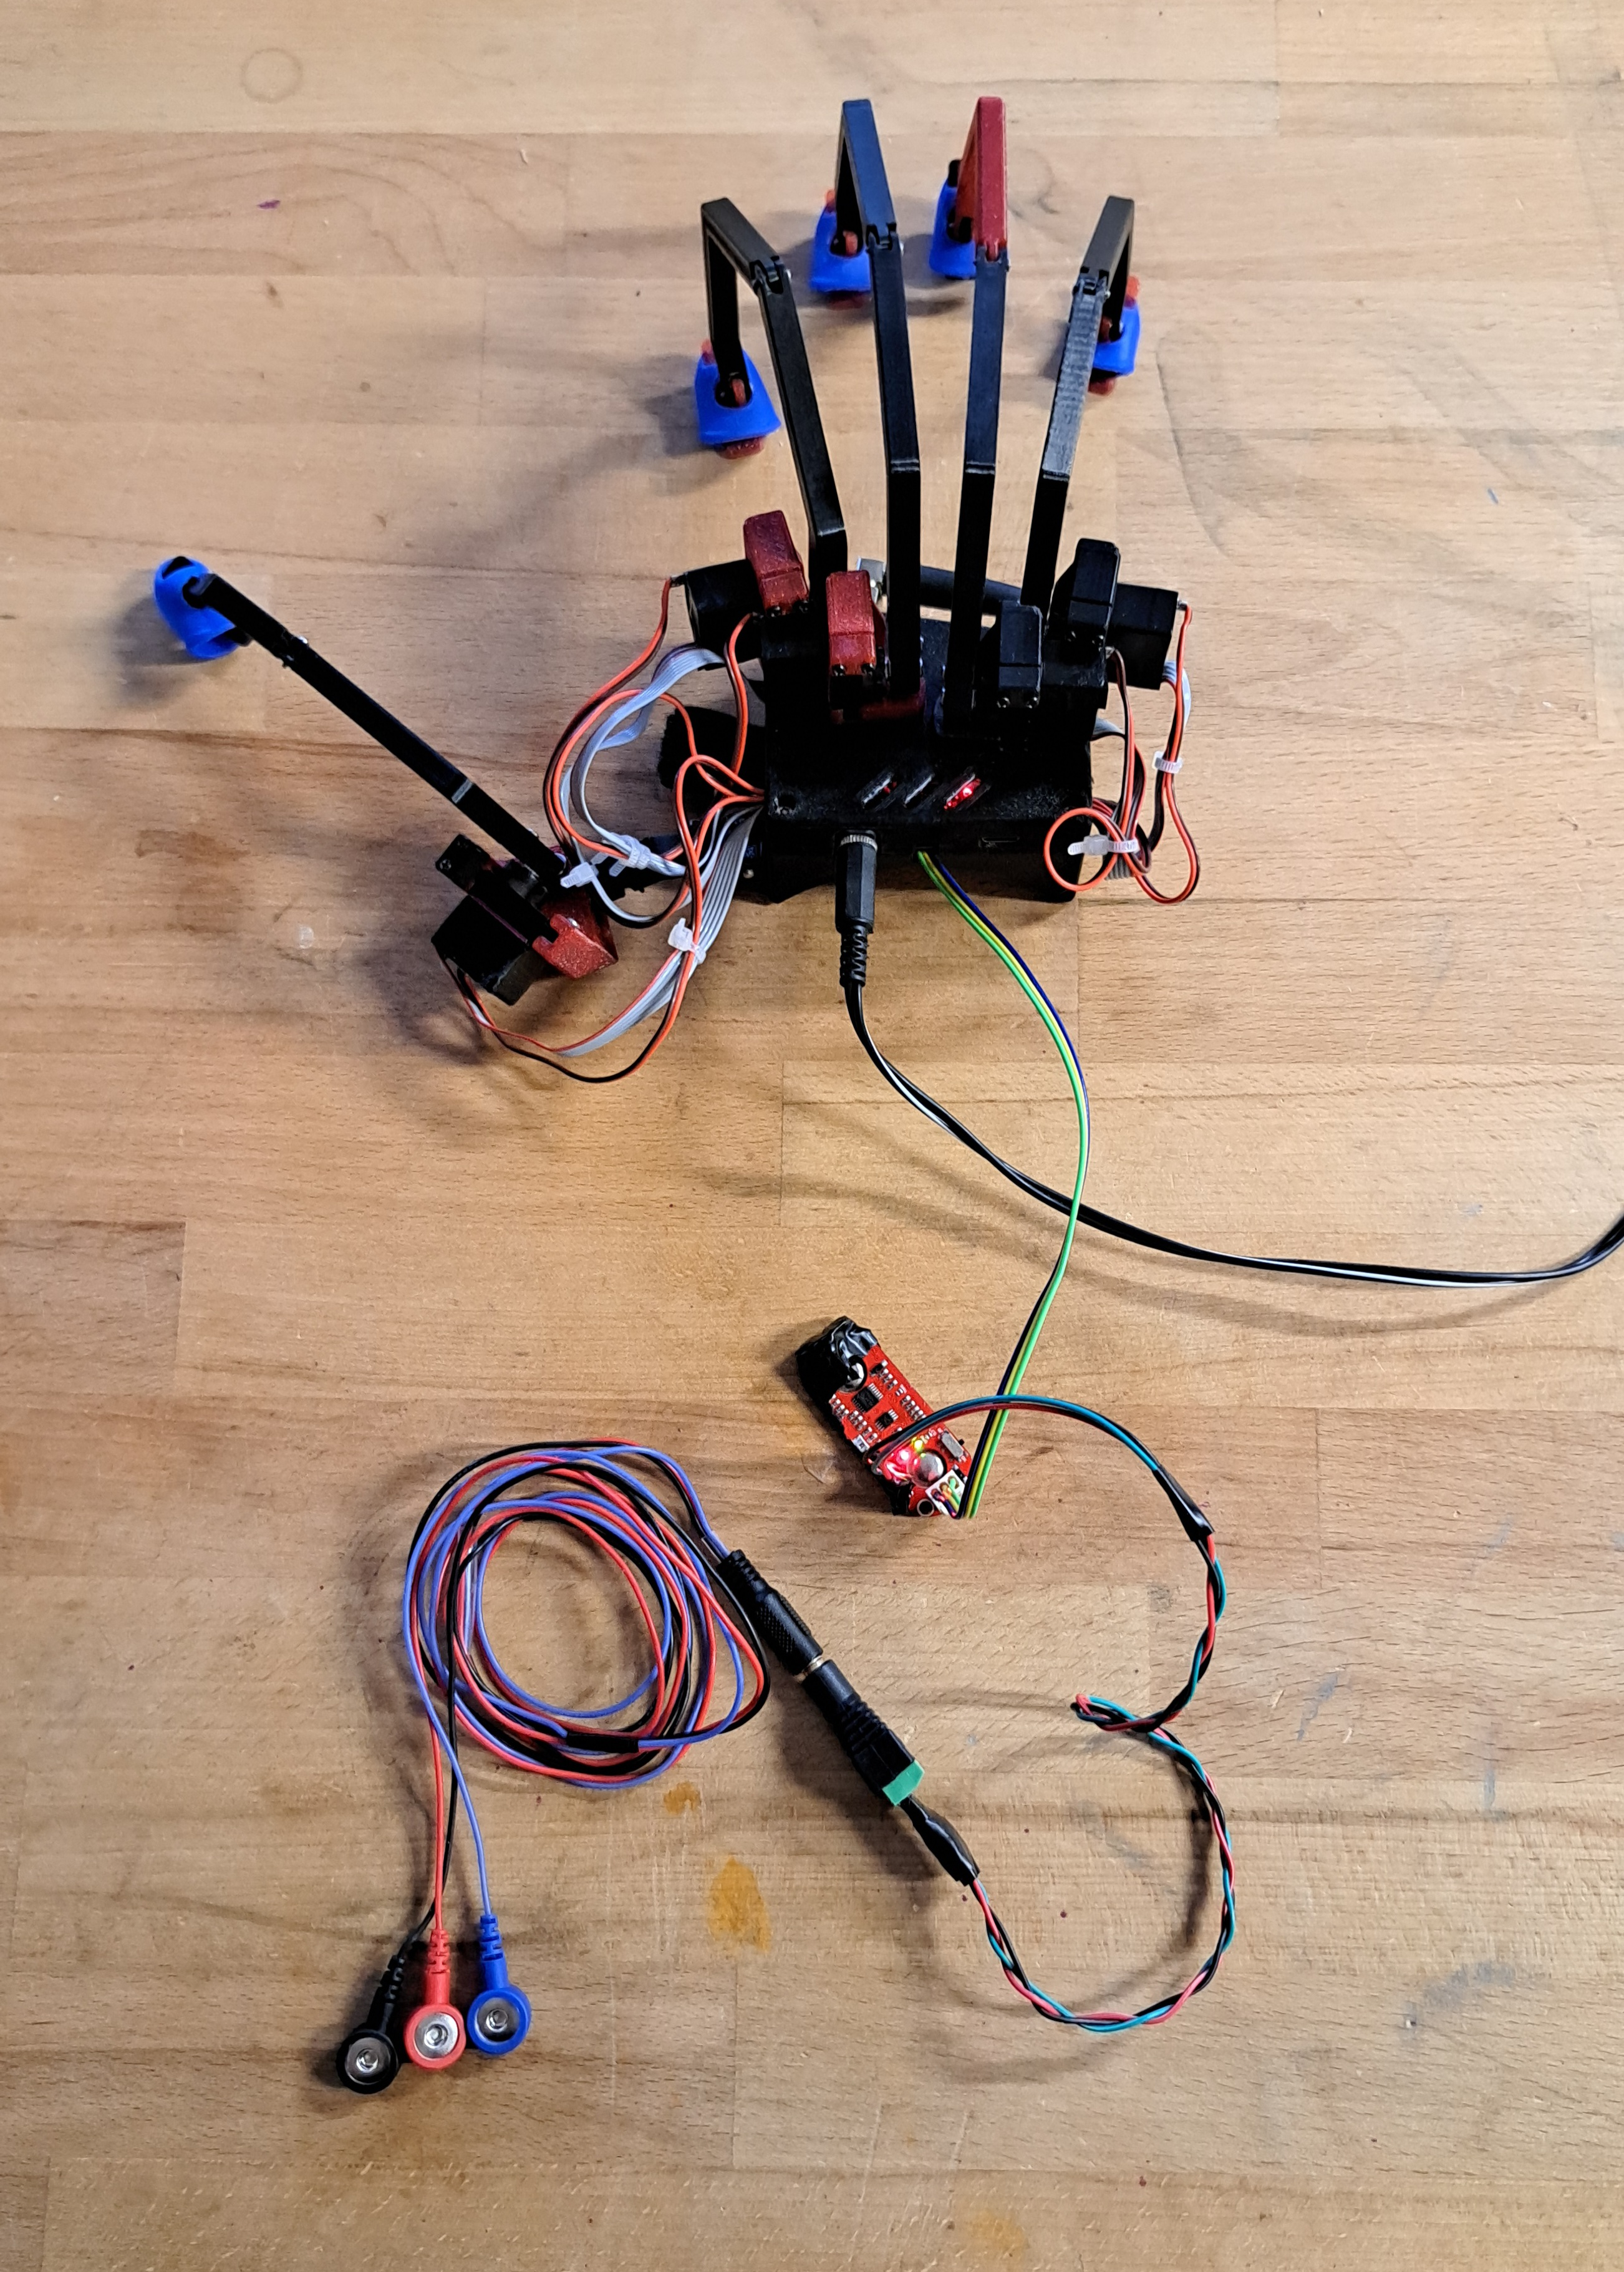
\includegraphics[width=0.42\textwidth]{Rukavice.jpg}
\caption{Realizovaná haptická rukavice Remote Feelings se senzorem sEMG.}
\label{fig:real-rukavice}
\end{figure}

\begin{figure}[H]
\centering
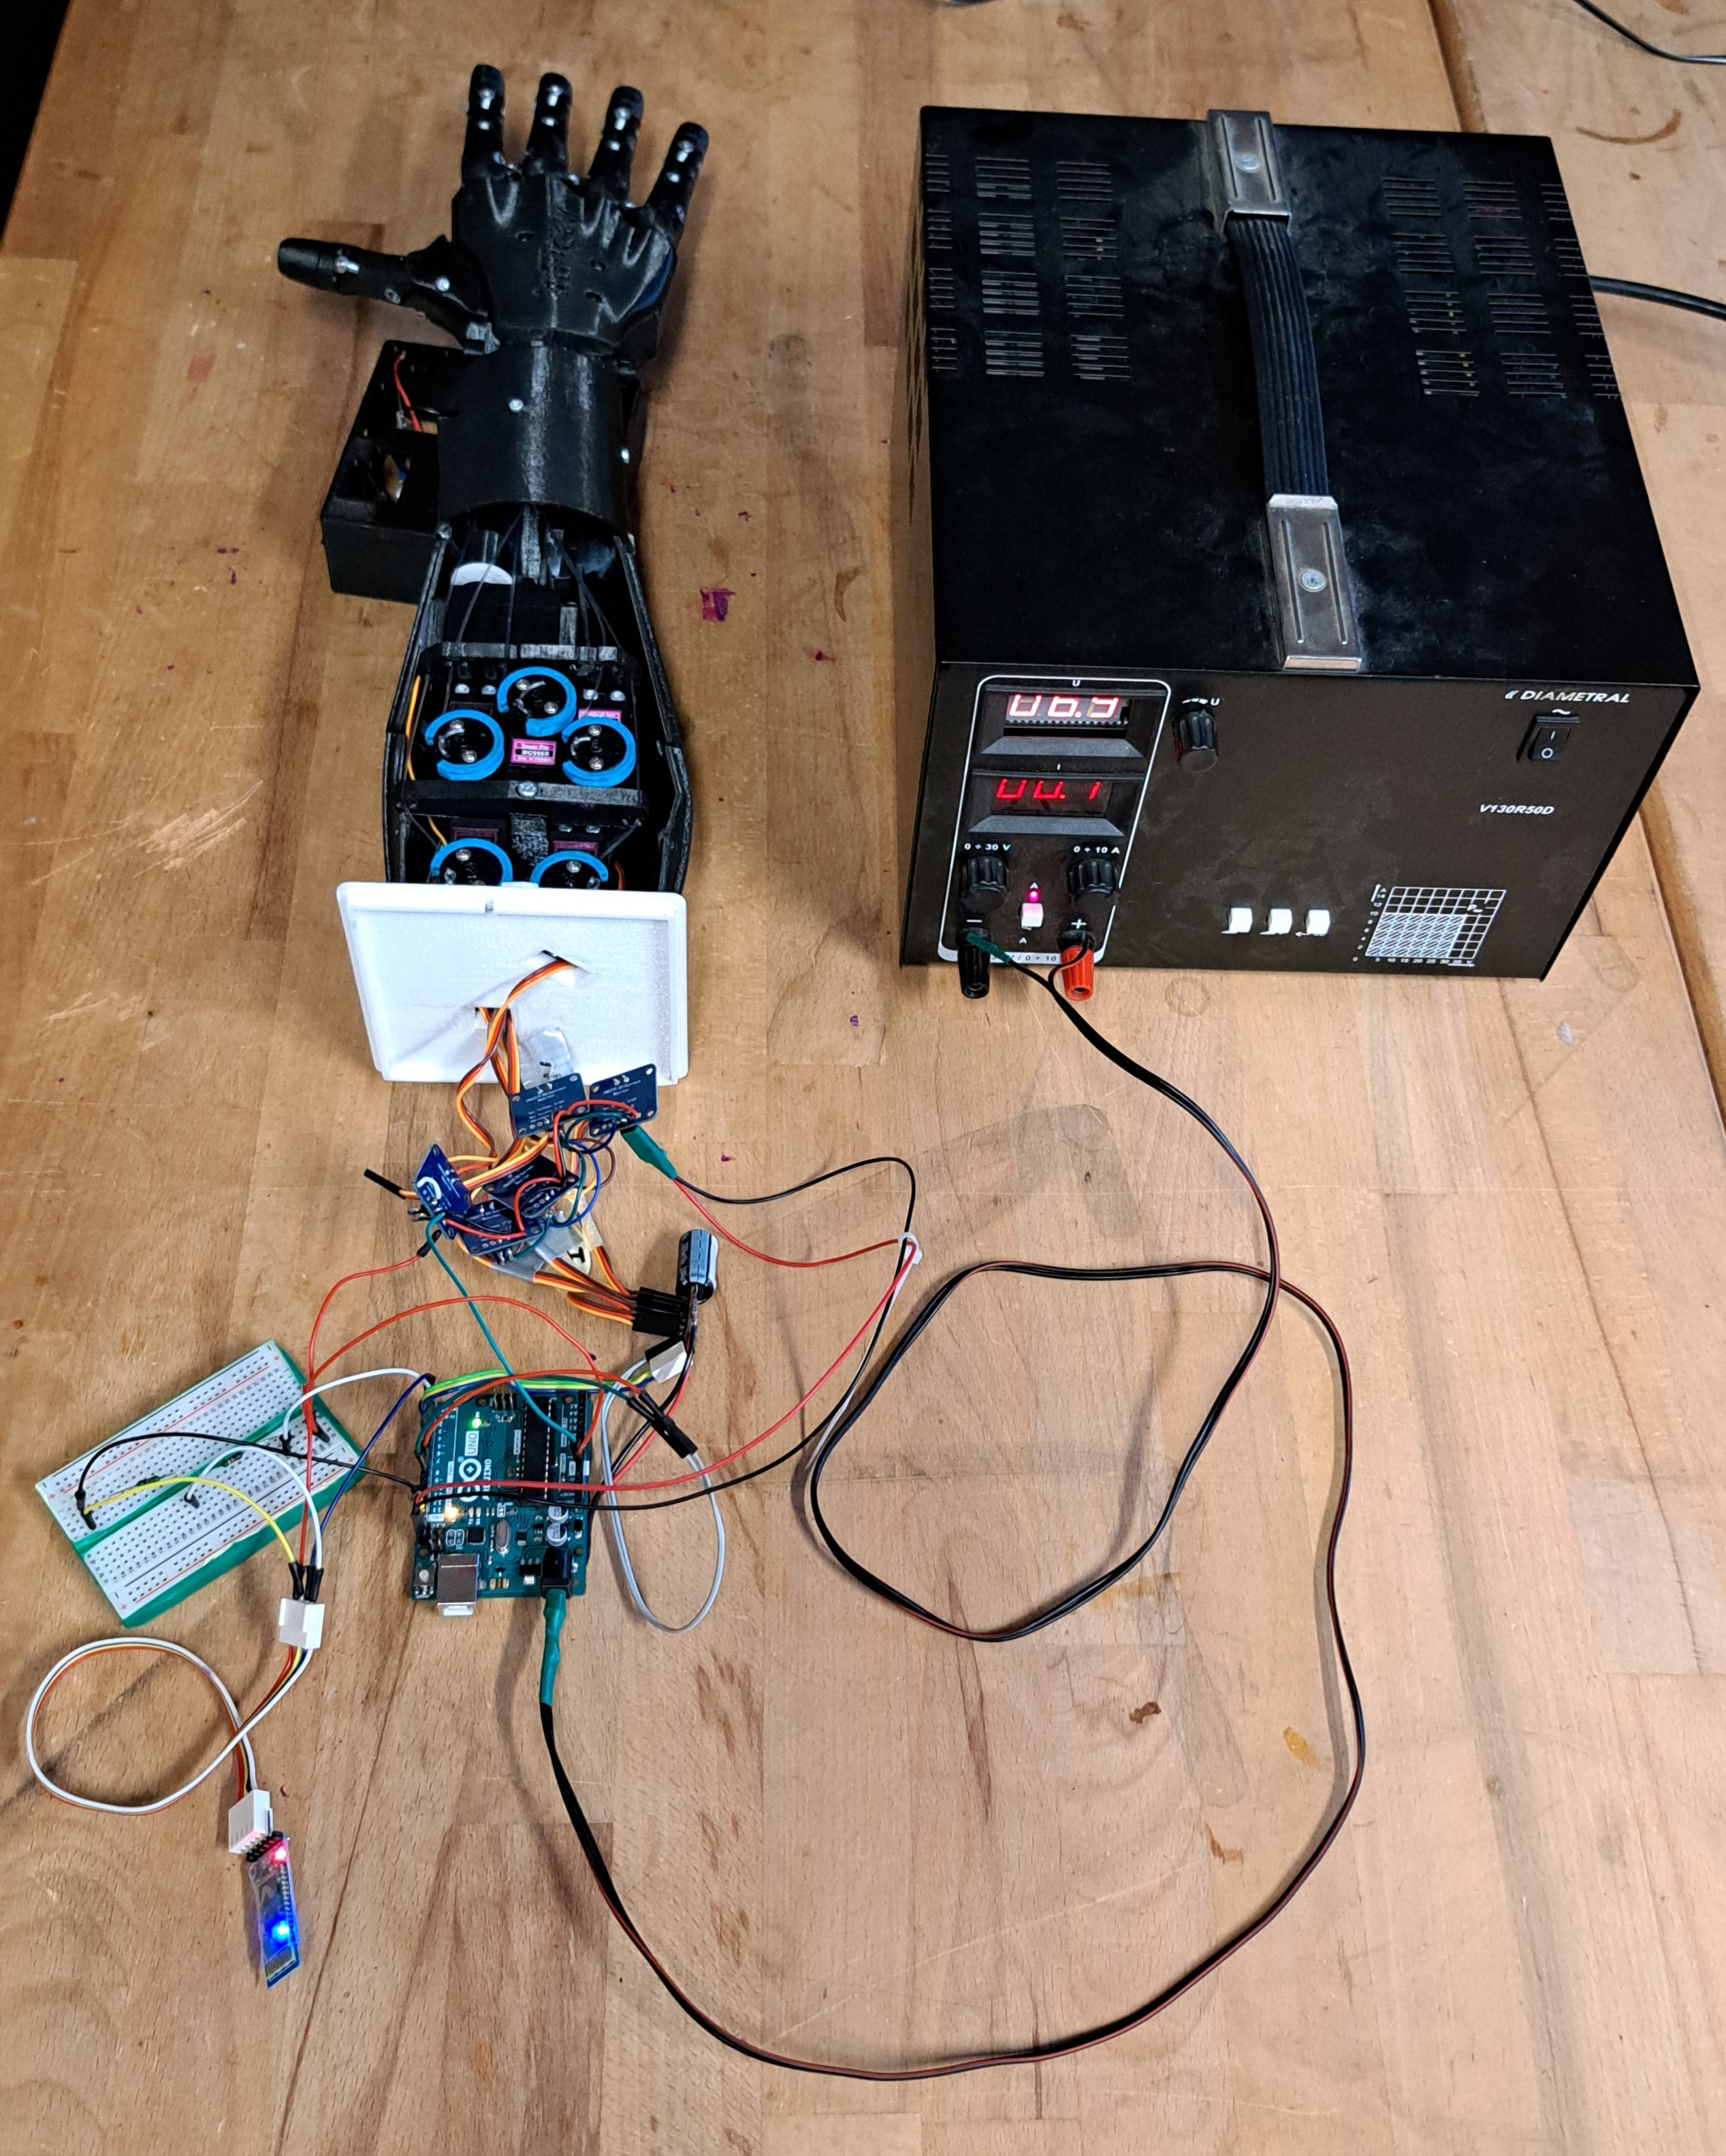
\includegraphics[width=0.42\textwidth]{Ruka.jpg}
\caption{Realizovaná robotická ruka InMoov s řídicí elektronikou a výkonovým zdrojem.}
\label{fig:real-inmoov}
\end{figure}

V realizované sestavě byly použity tyto hlavní části:

\begin{itemize}
    \item \textbf{ESP32-DevKitC V4} -- řídicí jednotka rukavice Remote Feelings; byly na ní zpracovávány signály FSR, polohové signály prstů, signál sEMG, lokální asistence prstů a haptická odezva,
    \item \textbf{Arduino UNO} -- řídicí jednotka robotické ruky InMoov; byly na ní přijímány řídicí pakety, řízeny servomotory a vyhodnocovány proudy jednotlivých serv,
    \item \textbf{HC-05} -- modul Bluetooth Classic připojený k hardwarovému UARTu Arduino UNO; ESP32 vystupovalo jako Bluetooth Master,
    \item \textbf{servomotory MG996R} -- pět aktuátorů robotické ruky InMoov napájených z odděleného výkonového zdroje 5--6\,V,
    \item \textbf{senzory INA219} -- pět proudových senzorů pro odhad zatížení servomotorů a detekci kontaktu,
    \item \textbf{senzory FSR} -- pět silově citlivých rezistorů v rukavici pro vyhodnocení lokálního pohybového záměru uživatele,
    \item \textbf{potenciometry, H-můstky a DC motory z upravených serv MG90S} -- prvky použité pro snímání polohy prstů a aktivní odpor v rukavici,
    \item \textbf{senzor MyoWare 1.0} -- analogový senzor povrchové elektromyografie pro doplňkové řízení robotické ruky signálem sEMG\@.
\end{itemize}

Blokové schéma subsystému robotické ruky InMoov je uvedeno na obr.~\ref{fig:inmoov-tok-signalu}. Tok signálů v rukavici Remote Feelings je rozdělen podle způsobu řízení a lokální asistence: režim MIRROR ukazuje obr.~\ref{fig:remote-feelings-mirror}, režim EMG obr.~\ref{fig:remote-feelings-emg} a aktivní asistenci pohybu prstů obr.~\ref{fig:remote-feelings-aktivni-asistence}.

% Diagram toku signalu pro system InMoov.
% V preambuli hlavniho dokumentu je potreba:
% \usepackage{tikz}
% \usetikzlibrary{arrows.meta, positioning, calc}
% \usepackage{float}

\begin{figure}[H]
    \centering
    \noindent\makebox[\linewidth][c]{%
    \resizebox{0.98\linewidth}{!}{%
    \begin{tikzpicture}[
        font=\normalsize,
        node distance=22mm and 18mm,
        block/.style={
            draw,
            rounded corners=2mm,
            align=center,
            minimum width=31mm,
            minimum height=14mm,
            fill=gray!8
        },
        controller/.style={block, fill=blue!10, thick},
        sensor/.style={block, fill=green!10},
        actuator/.style={block, fill=orange!14},
        object/.style={block, fill=yellow!18},
        bt/.style={block, fill=cyan!10, dashed},
        arrow/.style={
            -{Latex[length=3mm]},
            thick
        },
        feedbackarrow/.style={
            -{Latex[length=3mm]},
            thick,
            dashed,
            color=gray!70
        },
        labelabove/.style={
            midway, above=4mm,
            font=\small,
            fill=white, inner sep=2pt,
            text=black,
            align=center
        },
        labelbelow/.style={
            midway, below=4mm,
            font=\small,
            fill=white, inner sep=2pt,
            text=black,
            align=center
        },
        labeltext/.style={
            midway,
            font=\small,
            fill=white, inner sep=2pt,
            text=black,
            align=center
        }
    ]

    \node[bt] (btin) {Bluetooth\\z R.F.};
    \node[bt, right=of btin] (hc05) {HC-05};
    \node[controller, right=of hc05] (uno) {Arduino\\UNO};
    \node[actuator, right=of uno] (servos) {Servomotory\\InMoov};
    \node[block, right=of servos] (mech) {Mechanika\\InMoov};
    \node[object, right=of mech] (obj) {Držený\\předmět};

    \node[sensor, below=40mm of servos] (ina) {Senzory\\INA219};
    \node[bt, below=46mm of btin] (btout) {Bluetooth\\do R. F.};

    \draw[arrow] (btin) -- node[labelabove]{řídicí\\paket} (hc05);
    \draw[arrow] (hc05) to[bend left=12] node[labelabove]{UART} (uno);
    \draw[arrow] (uno) -- node[labelabove]{servo\\pulzy} (servos);
    \draw[arrow] (servos) to[bend left=12] node[labelabove]{tah lanek} (mech);
    \draw[arrow] (mech) to[bend left=12] node[labelabove]{úchop} (obj);

    \draw[arrow] (obj) to[bend left=12] node[labelbelow]{reakce objektu}(mech);
    \draw[arrow] (mech) to[bend left=12] node[labelbelow]{mechanická\\zátěž} (servos);

    \draw[arrow] (servos.south) -- node[labeltext, right=2mm]{odběr\\proudu} (ina.north);
    \draw[arrow] (ina.west) -- ++(-18mm,0)
        -| node[labelbelow, pos=0.22]{proud} (uno.south);

    \draw[arrow] (uno) to[bend left=12]
        node[labelbelow]{kontakt\\a intenzita} (hc05);
    \draw[arrow] (hc05.south) -- ++ (0,-46mm)
        |- node[labelbelow, pos=0.32]{UART / BT} (btout.east);

    \end{tikzpicture}
    }%
    }
    \caption{Tok signálů v systému robotické ruky InMoov.}
    \label{fig:inmoov-tok-signalu}
\end{figure}


% Diagram toku signalu pro Remote Feelings v rezimu MIRROR.
% V preambuli hlavniho dokumentu je potreba:
% \usepackage{tikz}
% \usetikzlibrary{arrows.meta, positioning, calc}
% \usepackage{float}

\begin{figure}[H]
    \centering
    \noindent\makebox[\linewidth][c]{%
    \resizebox{0.98\linewidth}{!}{%
    \begin{tikzpicture}[
        font=\normalsize,
        node distance=22mm and 18mm,
        block/.style={
            draw,
            rounded corners=2mm,
            align=center,
            minimum width=31mm,
            minimum height=14mm,
            fill=gray!8
        },
        controller/.style={block, fill=blue!10, thick},
        actuator/.style={block, fill=orange!14},
        person/.style={block, fill=yellow!18},
        bt/.style={block, fill=cyan!10, dashed},
        arrow/.style={
            -{Latex[length=3mm]},
            thick
        },
        feedbackarrow/.style={
            -{Latex[length=3mm]},
            thick,
            dashed,
            color=gray!70
        },
        labelabove/.style={
            midway, above=4mm,
            font=\small,
            fill=white, inner sep=2pt,
            text=black,
            align=center
        },
        labelbelow/.style={
            midway, below=4mm,
            font=\small,
            fill=white, inner sep=2pt,
            text=black,
            align=center
        },
        labeltext/.style={
            midway,
            font=\small,
            fill=white, inner sep=2pt,
            text=black,
            align=center
        }
    ]

    \node[person] (human) {Lidská\\ruka};
    \node[block, right=of human] (mechanics) {Mechanika\\R.F.};
    \node[actuator, right=of mechanics] (servos) {Servomotory\\R.F.};
    \node[controller, right=of servos] (esp) {ESP32-DevKitC V4};
    \node[bt, right=of esp] (btout) {Bluetooth\\do InMoov};

    \node[bt, below=28mm of btout] (btin) {Bluetooth\\z InMoov};

    \draw[arrow] (human) to[bend left=12] node[labelabove] {pohyb\\prstů} (mechanics);
    \draw[arrow] (mechanics) to[bend left=12] node[labelabove] {poloha\\prstů} (servos);
    \draw[arrow] (servos) to[bend left=12] node[labelabove] {stav\\rukavice} (esp);
    \draw[arrow] (esp) -- node[labelabove] {cílové polohy\\pro InMoov} (btout);

    \draw[arrow] (btin.west) -- ++(-8mm,0)
        |- node[labeltext, right=2mm, pos=0.3]{kontakt\\a intenzita} (esp.south east);
    \draw[arrow] (esp) to[bend left=12] node[labelbelow] {PWM\\odezvy} (servos);
    \draw[arrow] (servos) to[bend left=12] node[labelbelow] {protitah\\motorů} (mechanics);
    \draw[arrow] (mechanics) to[bend left=12] node[labelbelow] {haptický\\odpor} (human);



    \end{tikzpicture}
    }%
    }
    \caption{Tok signálů v systému Remote Feelings při režimu MIRROR.}
    \label{fig:remote-feelings-mirror}
\end{figure}


% Diagram toku signalu pro Remote Feelings v rezimu EMG.
% V preambuli hlavniho dokumentu je potreba:
% \usepackage{tikz}
% \usetikzlibrary{arrows.meta, positioning, calc}
% \usepackage{float}

\begin{figure}[H]
    \centering
    \noindent\makebox[\linewidth][c]{%
    \resizebox{0.98\linewidth}{!}{%
    \begin{tikzpicture}[
        font=\normalsize,
        node distance=22mm and 18mm,
        block/.style={
            draw,
            rounded corners=2mm,
            align=center,
            minimum width=31mm,
            minimum height=14mm,
            fill=gray!8
        },
        controller/.style={block, fill=blue!10, thick},
        sensor/.style={block, fill=green!10},
        actuator/.style={block, fill=orange!14},
        person/.style={block, fill=yellow!18},
        bt/.style={block, fill=cyan!10, dashed},
        arrow/.style={
            -{Latex[length=3mm]},
            thick
        },
        feedbackarrow/.style={
            -{Latex[length=3mm]},
            thick,
            dashed,
            color=gray!70
        },
        labelabove/.style={
            midway, above=4mm,
            font=\small,
            fill=white, inner sep=2pt,
            text=black,
            align=center
        },
        labelbelow/.style={
            midway, below=4mm,
            font=\small,
            fill=white, inner sep=2pt,
            text=black,
            align=center
        },
        labeltext/.style={
            midway,
            font=\small,
            fill=white, inner sep=2pt,
            text=black,
            align=center
        }
    ]

    \node[person] (human) {Lidská\\ruka};
    \node[sensor, right=of human] (emg) {sEMG\\senzor};
    \node[controller, right=of emg] (esp) {ESP32-DevKitC V4};
    \node[bt, right=of esp] (btout) {Bluetooth\\do InMoov};

    \node[actuator, below=28mm of esp] (servos) {Servomotory\\R.F.};
    \node[block, left=of servos] (mechanics) {Mechanika\\R.F.};
    \node[bt, right=of servos] (btin) {Bluetooth\\z InMoov};

    \draw[arrow] (human) -- node[labelabove]{svalová\\aktivita} (emg);
    \draw[arrow] (emg) -- node[labelabove]{raw sEMG} (esp);
    \draw[arrow] (esp) -- node[labelabove]{EMG data} (btout);

    \draw[feedbackarrow] (btout.east) -- ++(12mm,0)
        |- node[labeltext, right=2mm, pos=0.3]{systém\\InMoov} (btin.east);

    \draw[arrow] (btin.west) -- ++(-8mm,0)
        |- node[labeltext, right=2mm, pos=0.25]{kontakt\\a intenzita} (esp.south east);
    \draw[arrow] (esp.south) -- node[labeltext, right=2mm]{PWM\\odezvy} (servos.north);
    \draw[arrow] (servos) -- node[labelbelow]{protitah\\motorů} (mechanics);
    \draw[arrow] (mechanics.west) -- ++(-18mm,0)
        -| node[labelbelow, pos=0.22]{haptický\\odpor} (human.south);

    \end{tikzpicture}
    }%
    }
    \caption{Tok signálů v systému Remote Feelings při režimu EMG.}
    \label{fig:remote-feelings-emg}
\end{figure}


% Diagram aktivni asistence pohybu prstu v Remote Feelings.
% V preambuli hlavniho dokumentu je potreba:
% \usepackage{tikz}
% \usetikzlibrary{arrows.meta, positioning, calc}
% \usepackage{float}

\begin{figure}[H]
    \centering
    \noindent\makebox[\linewidth][c]{%
    \resizebox{0.98\linewidth}{!}{%
    \begin{tikzpicture}[
        font=\normalsize,
        node distance=22mm and 18mm,
        block/.style={
            draw,
            rounded corners=2mm,
            align=center,
            minimum width=31mm,
            minimum height=14mm,
            fill=gray!8
        },
        controller/.style={block, fill=blue!10, thick},
        sensor/.style={block, fill=green!10},
        actuator/.style={block, fill=orange!14},
        person/.style={block, fill=yellow!18},
        arrow/.style={
            -{Latex[length=3mm]},
            thick
        },
        feedbackarrow/.style={
            -{Latex[length=3mm]},
            thick,
            dashed,
            color=gray!70
        },
        labelabove/.style={
            midway, above=4mm,
            font=\small,
            fill=white, inner sep=2pt,
            text=black,
            align=center
        },
        labelbelow/.style={
            midway, below=4mm,
            font=\small,
            fill=white, inner sep=2pt,
            text=black,
            align=center
        },
        labeltext/.style={
            midway,
            font=\small,
            fill=white, inner sep=2pt,
            text=black,
            align=center
        }
    ]

    \node[person] (human) {Lidská\\ruka};
    \node[block, right=of human] (mechanics) {Mechanika\\R.F.};
    \node[sensor, right=of mechanics] (fsr) {FSR\\senzory};
    \node[controller, right=of fsr] (esp) {ESP32-DevKitC V4};
    \node[actuator, right=of esp] (servos) {Servomotory\\R.F.};

    \draw[arrow] (human) to[bend left=12] node[labelabove] {pohyb\\prstů} (mechanics);
    \draw[arrow] (mechanics) -- node[labelabove] {tlak\\na FSR} (fsr);
    \draw[arrow] (fsr) -- node[labelabove] {záměr\\pohybu} (esp);
    \draw[arrow] (esp) -- node[labelabove] {PWM} (servos);
    \draw[arrow] (servos.south) -- ++(0,-18mm)
        -| node[labelbelow, pos=0.25] {asistenční\\síla} (mechanics.south);
    \draw[arrow] (mechanics) to[bend left=12] node[labelbelow] {podpora\\pohybu} (human);

    \end{tikzpicture}
    }%
    }
    \caption{Tok signálů při aktivní asistenci pohybu prstů v rukavici Remote Feelings.}
    \label{fig:remote-feelings-aktivni-asistence}
\end{figure}


Přenos dat byl realizován oběma směry. Z ESP32 do Arduino UNO byly odesílány cílové úhly servomotorů, hodnoty sEMG a zvolený režim řízení. Z Arduino UNO do ESP32 byly odesílány aktuální polohy serv, filtrované proudy, bitová maska kontaktu a intenzity kontaktu. Synchronizace paketů byla provedena dvojicí hlavičkových bajtů \texttt{0xAA} a \texttt{0xBB}. Struktury paketů byly sdíleny v hlavičkovém souboru \texttt{telemetry.h}, který musel být udržován identicky ve firmware obou mikrokontrolérů.

Výchozím bodem návrhu byl původní firmware rukavice Remote Feelings publikovaný Curtisem et al.~\cite{Curtis2021}. Tento firmware byl koncipován jako samostatný prototyp zaměřený na lokální práci s FSR senzory, potenciometry a H-můstky s jednoduchou textovou sériovou komunikací. Neobsahoval sEMG vstup, obousměrný Bluetooth protokol ani silovou zpětnou vazbu po jednotlivých prstech. Navržený systém z tohoto základu vychází, ale rozšiřuje ho do bilaterální konfigurace Leader--Follower se dvěma řídicími jednotkami, binárním paketem sdíleným přes Bluetooth a haptickou stěnou odvozenou z proudové telemetrie robotické ruky.

\section{Návrhové požadavky a omezení}
\label{sec:pozadavky-omezeni}

Před návrhem systému byly stanoveny požadavky vyplývající z cíle práce. Sestava neměla sloužit pouze jako jednostranné dálkové ovládání robotické ruky, ale jako obousměrný teleoperační systém umožňující řízení, měření a zpětnovazební odezvu. Základní požadavky jsou shrnuty v tabulce~\ref{tab:pozadavky-system}.

\begin{table}[H]
\centering
\caption{Návrhové požadavky na realizovaný systém}
\label{tab:pozadavky-system}
\begin{tabular}{|p{0.32\textwidth}|p{0.58\textwidth}|}
\hline
\textbf{Požadavek} & \textbf{Důvod a dopad na návrh} \\
\hline
Pět samostatně ovládaných prstů & Robotická ruka i rukavice obsahovaly pět prstových kanálů. V režimu MIRROR byla poloha každého prstu přenášena samostatně, zatímco režim EMG byl omezen jedním sEMG kanálem. \\
\hline
Obousměrná komunikace & Do robotické ruky bylo nutné přenášet řídicí data a zpět do rukavice proudovou telemetrii i kontaktní informaci. \\
\hline
Nízká latence & Pohyb robotické ruky a haptická odezva měly být vnímány jako spojitá reakce systému. \\
\hline
Bezpečné chování při poruše & Při resetu ESP32, výpadku Bluetooth nebo nedokončeném paketu nesměl nastat nekontrolovaný pohyb motorů ani dlouhodobé sevření robotické ruky. \\
\hline
Oddělení výkonové a řídicí části & Servomotory byly napájeny z externího zdroje. Se signálovou elektronikou byla sdílena zem, ale proudové špičky nebyly vedeny přes USB ani přes desku Arduino UNO\@. \\
\hline
Kalibrace pro aktuálního uživatele & Poloha prstů, přítlak FSR senzorů i rozsah sEMG se měnily podle nasazení rukavice a kontaktu elektrod s pokožkou. \\
\hline
Využití dostupného hardwaru & Návrh byl omezen použitými deskami, modulem HC-05, servomotory MG996R, upravenými servy MG90S a proudovými senzory INA219. \\
\hline
\end{tabular}
\end{table}

Z uvedených požadavků vyplynul kompromis mezi jednoduchostí a robustností. Na Arduino UNO byla ponechána pouze časově kritická a jednodušší část úlohy: příjem paketů, řízení serv, měření proudů a odesílání telemetrie. Na ESP32 byla umístěna výpočetně náročnější část, zejména čtení senzorů rukavice, kalibrace, aktivní asistence, sEMG zpracování a haptická reakce.

\section{Tok signálu v systému}
\label{sec:tok-signalu}

Tok signálů byl rozdělen podle provozních režimů. V režimu MIRROR byla poloha prstů snímána potenciometry v rukavici, převedena na cílové úhly a odeslána do robotické ruky. V režimu EMG byl pohybový povel odvozen ze signálu povrchové elektromyografie. V obou režimech byla na straně robotické ruky současně měřena proudová odezva servomotorů a tato informace byla využita pro odhad kontaktu.

Schématicky lze celý řetězec popsat následovně:

\begin{enumerate}
    \item v rukavici byly snímány polohy prstů, lokální zatížení FSR senzorů a sEMG signál,
    \item na ESP32 byla provedena kalibrace, filtrace a výběr režimu řízení,
    \item binární paket byl odeslán přes Bluetooth Classic do Arduino UNO,
    \item na Arduino UNO byly vypočteny řídicí pulzy serv robotické ruky,
    \item proud každého serva byl měřen senzorem INA219 a filtrován,
    \item při detekci nadproudu byl vytvořen kontaktový stav a intenzita kontaktu,
    \item telemetrický paket byl odeslán zpět do ESP32,
    \item v rukavici byla podle kontaktové informace aktivována haptická stěna.
\end{enumerate}

Na tento slovní popis navazují bloková schémata zařazená v části~\ref{sec:celkova-architektura}, která odděleně ukazují tok signálů v robotické ruce InMoov, v režimu MIRROR, v režimu EMG a při aktivní asistenci pohybu prstů.

\section{Přehled zapojení a pinout}
\label{sec:pinout}

Přehled pinů byl sestaven podle finálního firmwaru. Na straně ESP32 bylo v programu použito interní pořadí prstů malíček, prsteník, prostředník, ukazovák a palec. Na straně Arduino UNO bylo pořadí serv odlišné: palec, ukazovák, prostředník, prsteník a malíček. Převod mezi těmito konvencemi byl řešen v komunikační vrstvě.

\begin{table}[H]
\centering
\caption{Pinout ESP32-DevKitC V4 v rukavici Remote Feelings}
\label{tab:pinout-esp32}
\begin{tabular}{|p{0.15\textwidth}|p{0.17\textwidth}|p{0.17\textwidth}|p{0.26\textwidth}|p{0.15\textwidth}|}
\hline
\textbf{Prst} & \textbf{FSR ADC} & \textbf{Poloha ADC} & \textbf{H-můstek IN1/IN2} & \textbf{Poznámka} \\
\hline
Malíček & GPIO36 & GPIO4 & GPIO17 / GPIO16 & GPIO36 je pouze vstup. \\
\hline
Prsteník & GPIO39 & GPIO26 & GPIO22 / GPIO21 & GPIO39 je pouze vstup. \\
\hline
Prostředník & GPIO34 & GPIO27 & GPIO18 / GPIO19 & GPIO34 je pouze vstup. \\
\hline
Ukazovák & GPIO35 & GPIO14 & GPIO23 / GPIO5 & GPIO35 je pouze vstup. \\
\hline
Palec & GPIO32 & GPIO13 & GPIO12 / GPIO15 & ADC vstup ESP32. \\
\hline
\end{tabular}
\end{table}

\begin{table}[H]
\centering
\caption{Další signály na straně ESP32}
\label{tab:pinout-esp32-dalsi}
\begin{tabular}{|p{0.30\textwidth}|p{0.22\textwidth}|p{0.38\textwidth}|}
\hline
\textbf{Signál} & \textbf{Pin ESP32} & \textbf{Poznámka} \\
\hline
sEMG MyoWare SIG & GPIO33 (ADC1) & Byl použit vstup ADC1, protože ADC2 může být omezen při aktivním bezdrátovém spojení. \\
\hline
USB Serial monitor & USB převodník desky & Rychlost 115200 Bd; rozhraní bylo využito pro ovládací příkazy a ladění. \\
\hline
Bluetooth Classic & interní rádio ESP32 & ESP32 bylo nakonfigurováno jako Bluetooth Master a připojovalo se k MAC adrese HC-05. \\
\hline
\end{tabular}
\end{table}

Praktické provedení řídicí desky rukavice s modulem ESP32 a konektory pro senzory a aktuátory je zachyceno na obr.~\ref{fig:rukavice-pcb}.

\begin{figure}[H]
\centering
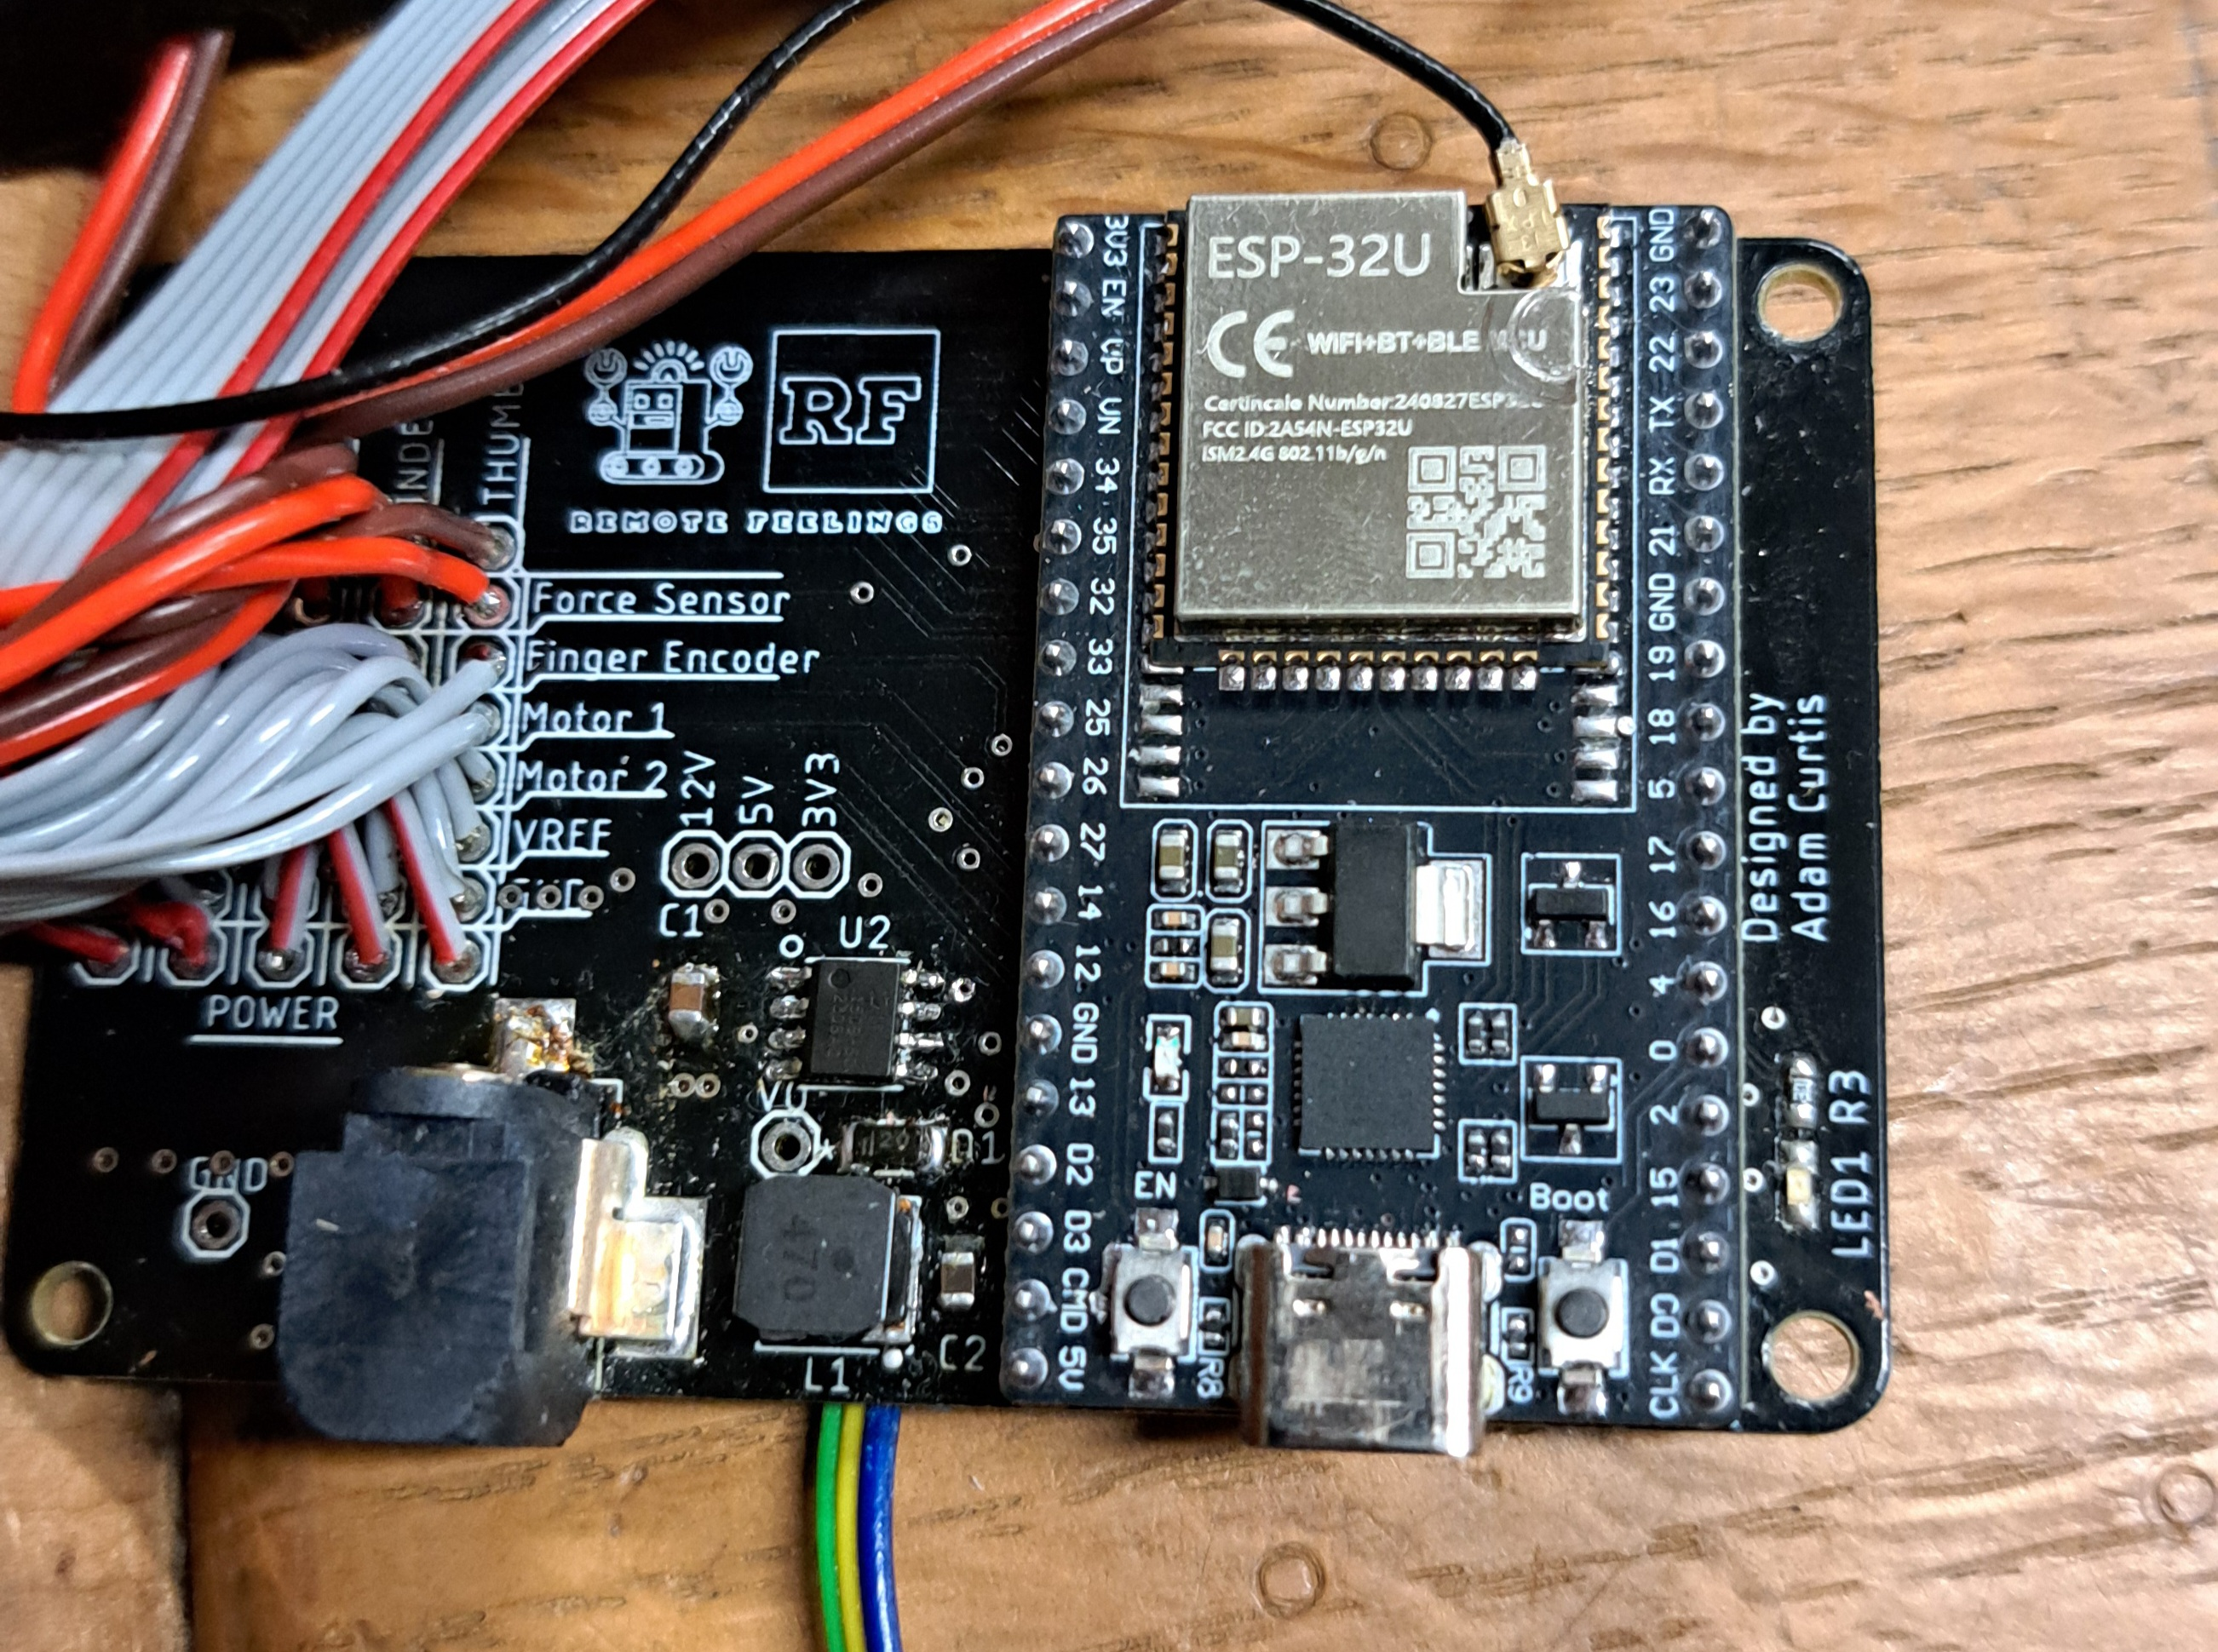
\includegraphics[width=0.82\textwidth]{Rukavice_PCB.jpg}
\caption{Deska rukavice Remote Feelings s modulem ESP32 a konektory pro připojení senzorů a motorů.}
\label{fig:rukavice-pcb}
\end{figure}

\begin{table}[H]
\centering
\caption{Pinout Arduino UNO v robotické ruce InMoov}
\label{tab:pinout-arduino}
\begin{tabular}{|p{0.27\textwidth}|p{0.21\textwidth}|p{0.42\textwidth}|}
\hline
\textbf{Funkce} & \textbf{Pin Arduino UNO} & \textbf{Poznámka} \\
\hline
Servo palce & D8 & Řídicí pulzy serva MG996R. \\
\hline
Servo ukazováku & D9 & Řídicí pulzy serva MG996R. \\
\hline
Servo prostředníku & D2 & Řídicí pulzy serva MG996R. \\
\hline
Servo prsteníku & D3 & Řídicí pulzy serva MG996R. \\
\hline
Servo malíčku & D4 & Řídicí pulzy serva MG996R. \\
\hline
HC-05 TX $\rightarrow$ Arduino RX & D0 & Přijímaná data z modulu Bluetooth. \\
\hline
Arduino TX $\rightarrow$ HC-05 RX & D1 & Bylo použito přizpůsobení úrovní odporovým děličem 1\,k$\Omega$ / 2\,k$\Omega$. \\
\hline
I2C SDA & A4 & Společná sběrnice pro pět modulů INA219. \\
\hline
I2C SCL & A5 & Společná sběrnice pro pět modulů INA219. \\
\hline
\end{tabular}
\end{table}

\begin{table}[H]
\centering
\caption{Napájecí větve a společná zem systému}
\label{tab:napajeci-vetve}
\begin{tabular}{|p{0.32\textwidth}|p{0.58\textwidth}|}
\hline
\textbf{Větev} & \textbf{Zapojení a význam} \\
\hline
Logika ESP32 a senzory rukavice & ESP32 bylo napájeno přes USB nebo stabilizovaný vstup. Senzor MyoWare i analogové děliče FSR byly napájeny napětím 3,3\,V, aby nebyly překročeny vstupní limity ADC. \\
\hline
Motory a H-můstky rukavice & Výkonová část byla vedena odděleně od signálových vodičů. Řídicí vstupy H-můstků byly staženy rezistory 10\,k$\Omega$ k zemi. \\
\hline
Arduino UNO a HC-05 & Arduino UNO napájelo logickou část a modul HC-05. Modul HC-05 byl připojen na D0/D1, proto musel být při nahrávání firmware odpojen. \\
\hline
Serva InMoov & Servomotory MG996R byly napájeny z externího zdroje 5--6\,V. Kvůli proudovým špičkám byla vhodná proudová rezerva 10--15\,A. \\
\hline
Společná zem & Všechny signálové části a výkonové zdroje musely sdílet GND, aby byly definovány úrovně PWM, UART i I2C signálů. \\
\hline
\end{tabular}
\end{table}

\section{Senzorická a aktuační část rukavice}
\label{sec:snimaci-cast-rukavice}

Senzorická část rukavice byla tvořena třemi modalitami: silově citlivými rezistory FSR, polohovými potenciometry z upravených servomechanismů a senzorem povrchové elektromyografie MyoWare 1.0. FSR senzory byly použity pro lokální asistenci prstů, potenciometry pro polohové řízení režimu MIRROR a sEMG senzor pro alternativní řízení robotické ruky. Aktuační část rukavice, tvořená DC motory a H-můstky z upravených serv MG90S, je popsána v části~\ref{sec:hapticka-rukavice}.

\subsection{Silově citlivé senzory FSR}
\label{subsec:fsr}

Na každý prst rukavice byl umístěn silově citlivý rezistor. Tímto senzorem nebyla měřena svalová kontrakce přímo, ale změna mechanického tlaku nebo deformace v konstrukci rukavice. Pohybový záměr uživatele byl z hodnoty FSR pouze odvozován: při snaze prst zavřít nebo otevřít se změnilo zatížení konstrukce a tato změna byla vyhodnocena firmwarem ESP32.

Senzory byly zapojeny do dělicího obvodu s referenčním rezistorem a výstupní napětí bylo přivedeno na dvanáctibitové ADC vstupy ESP32. Surové hodnoty byly během kalibrace přiřazeny ke klidovému stavu, směru zavírání a směru otevírání. Před vyhodnocením byl signál filtrován exponenciálním klouzavým průměrem
\begin{equation}
    y_k = \alpha x_k + \left(1 - \alpha\right)y_{k-1},
\end{equation}
kde $\alpha$ označuje filtrační konstantu zvolenou podle frekvence řídicí smyčky.

Výstup filtru byl porovnáván s adaptivní mrtvou zónou \texttt{DEADZONE[i]}. Její hodnota byla odvozena z klidového šumu senzoru podle vztahu
\begin{equation}
    \mathrm{DEADZONE}_i =
    \mathrm{constrain}\left(6\Delta_{\mathrm{šum}},\;15,\;150\right),
\end{equation}
kde $\Delta_{\mathrm{šum}}$ představuje rozsah špička--špička ve fázi klidové kalibrace. Touto úpravou byly potlačeny falešné aktivace způsobené elektrickým a mechanickým šumem.

\subsection{Polohové potenciometry a H-můstky}
\label{subsec:potenciometry-hmustky}

Poloha každého prstu rukavice byla snímána potenciometrem získaným z upraveného servomotoru MG90S 180$^\circ$. Běžný servomechanismus byl rozdělen na tři samostatně využitelné části: potenciometr, DC motor a řídicí H-můstek. Potenciometr byl vyveden na vstupy ADC ESP32, zatímco DC motor a H-můstek byly použity pro aktivní působení na prst rukavice.

Každý prst měl v paměti uložené krajní kalibrační hodnoty \texttt{fingerPosMin[]} a \texttt{fingerPosMax[]}. U prostředníku a ukazováku byl z mechanických důvodů směr potenciometru obrácen, takže bylo nutné v softwaru zohlednit i případ \texttt{fingerPosMin > fingerPosMax}. Řídicí signály pro H-můstky byly vedeny z ESP32 na vstupy IN\@. Na těchto vodičích byly osazeny pull-down rezistory 10\,k$\Omega$, aby při resetu ESP32 nebo při nahrávání firmware nevznikal nedefinovaný stav vedoucí k samovolnému pohybu motorů.

\begin{figure}[H]
\centering
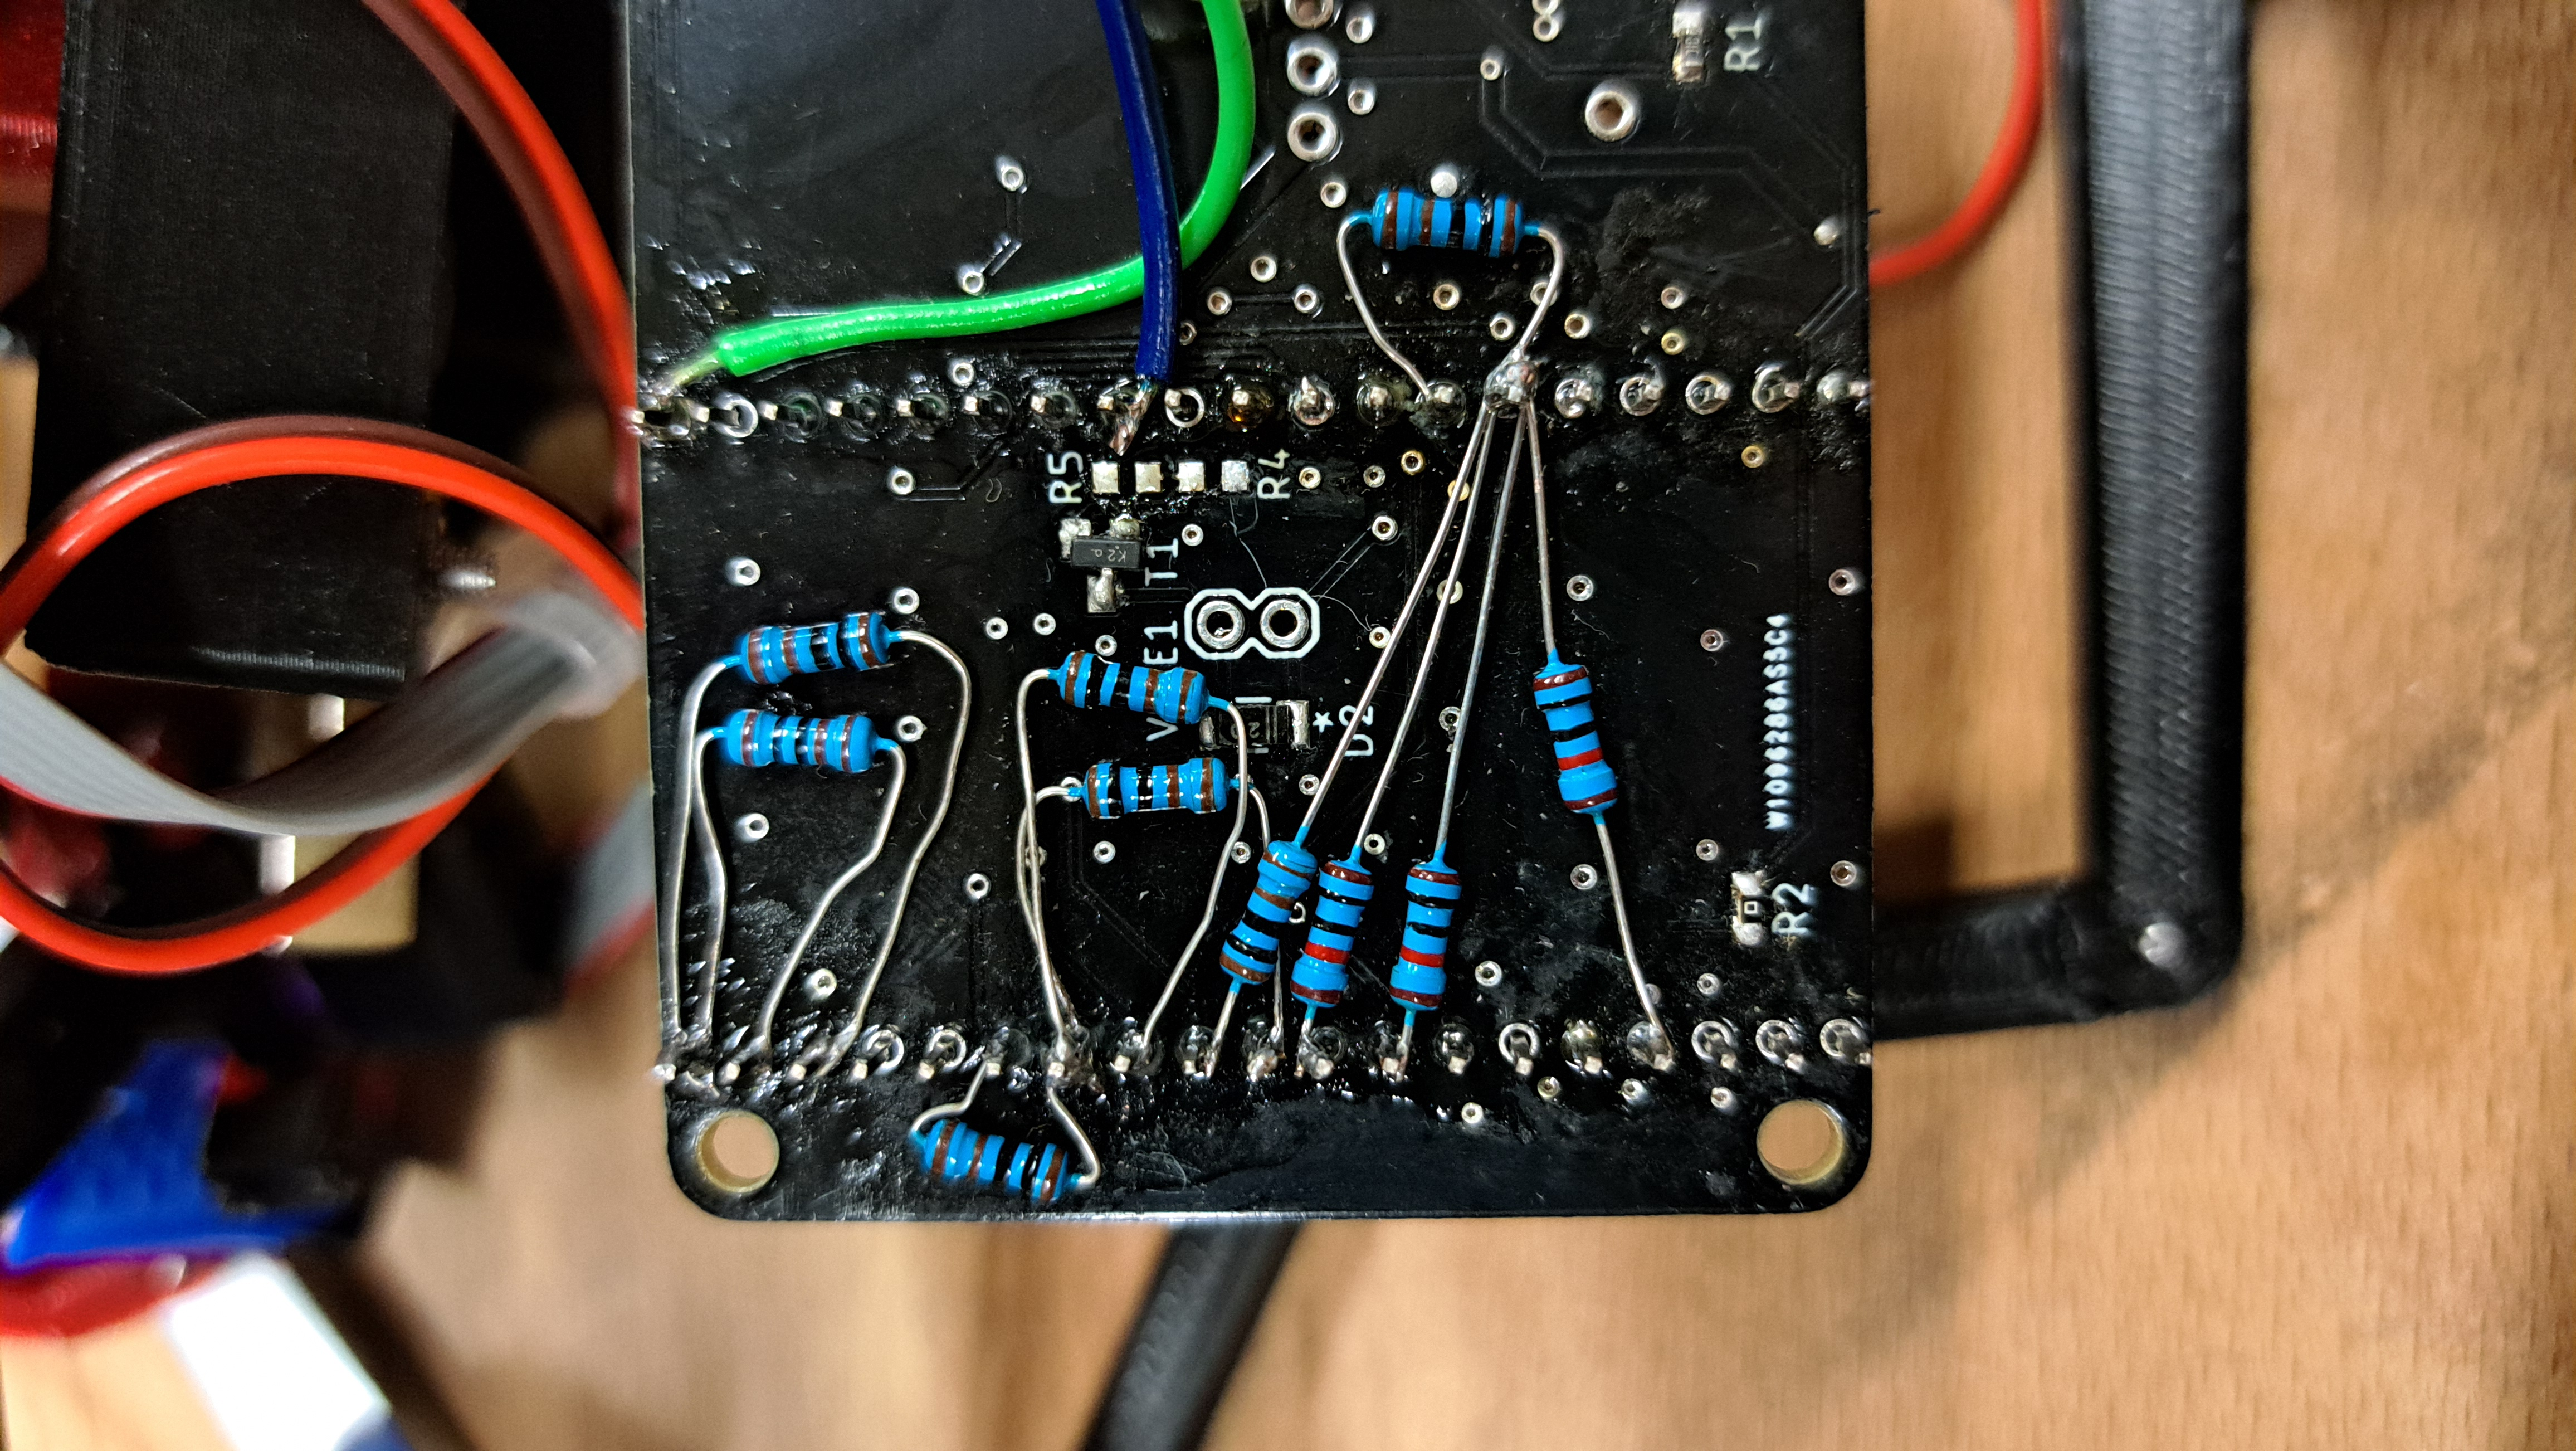
\includegraphics[width=0.82\textwidth]{pull-down_rezistory.jpg}
\caption{Doplněné pull-down rezistory na vodičích řídicích vstupů H-můstků rukavice.}
\label{fig:pull-down-rezistory}
\end{figure}

\subsection{Senzor povrchové elektromyografie MyoWare 1.0}
\label{subsec:myoware}

Pro alternativní režim řízení byl integrován analogový senzor povrchové elektromyografie MyoWare 1.0. Výstup senzoru byl přiveden na GPIO33, tedy na vstup ADC1 desky ESP32 \cite{espressif_adc}. Tento vstup byl vybrán kvůli stabilnějšímu měření při současně aktivním bezdrátovém spojení. Původně uvažovaný vstup GPIO25 patří k ADC2, jehož použití může být při práci s bezdrátovou částí ESP32 problematické.

Senzor byl napájen z pinu 3V3. Napájení z 5\,V nebylo použito, protože výstup SIG by při maximální svalové kontrakci mohl dosáhnout 5\,V a překročit maximální povolené vstupní napětí ADC ESP32.

\begin{table}[H]
\centering
\caption{Zapojení senzoru MyoWare 1.0 k desce ESP32-DevKitC V4}
\label{tab:myoware}
\begin{tabular}{|p{0.20\textwidth}|p{0.25\textwidth}|p{0.45\textwidth}|}
\hline
\textbf{Pin MyoWare} & \textbf{Pin ESP32} & \textbf{Poznámka} \\
\hline
\texttt{+} (VCC) & \texttt{3V3} & Napájení 3,3\,V. \\
\hline
\texttt{-} (GND) & \texttt{GND} & Společná zem se systémem. \\
\hline
\texttt{SIG} & GPIO33 (ADC1) & Analogový vstup pro sEMG signál. \\
\hline
\end{tabular}
\end{table}

Zapojení vodičů senzoru MyoWare do desky rukavice je dokumentováno na obr.~\ref{fig:zapojeni-emg}. Umístění elektrod na předloktí při použití rukavice je znázorněno na obr.~\ref{fig:rukavice-emg}.

\begin{figure}[H]
\centering
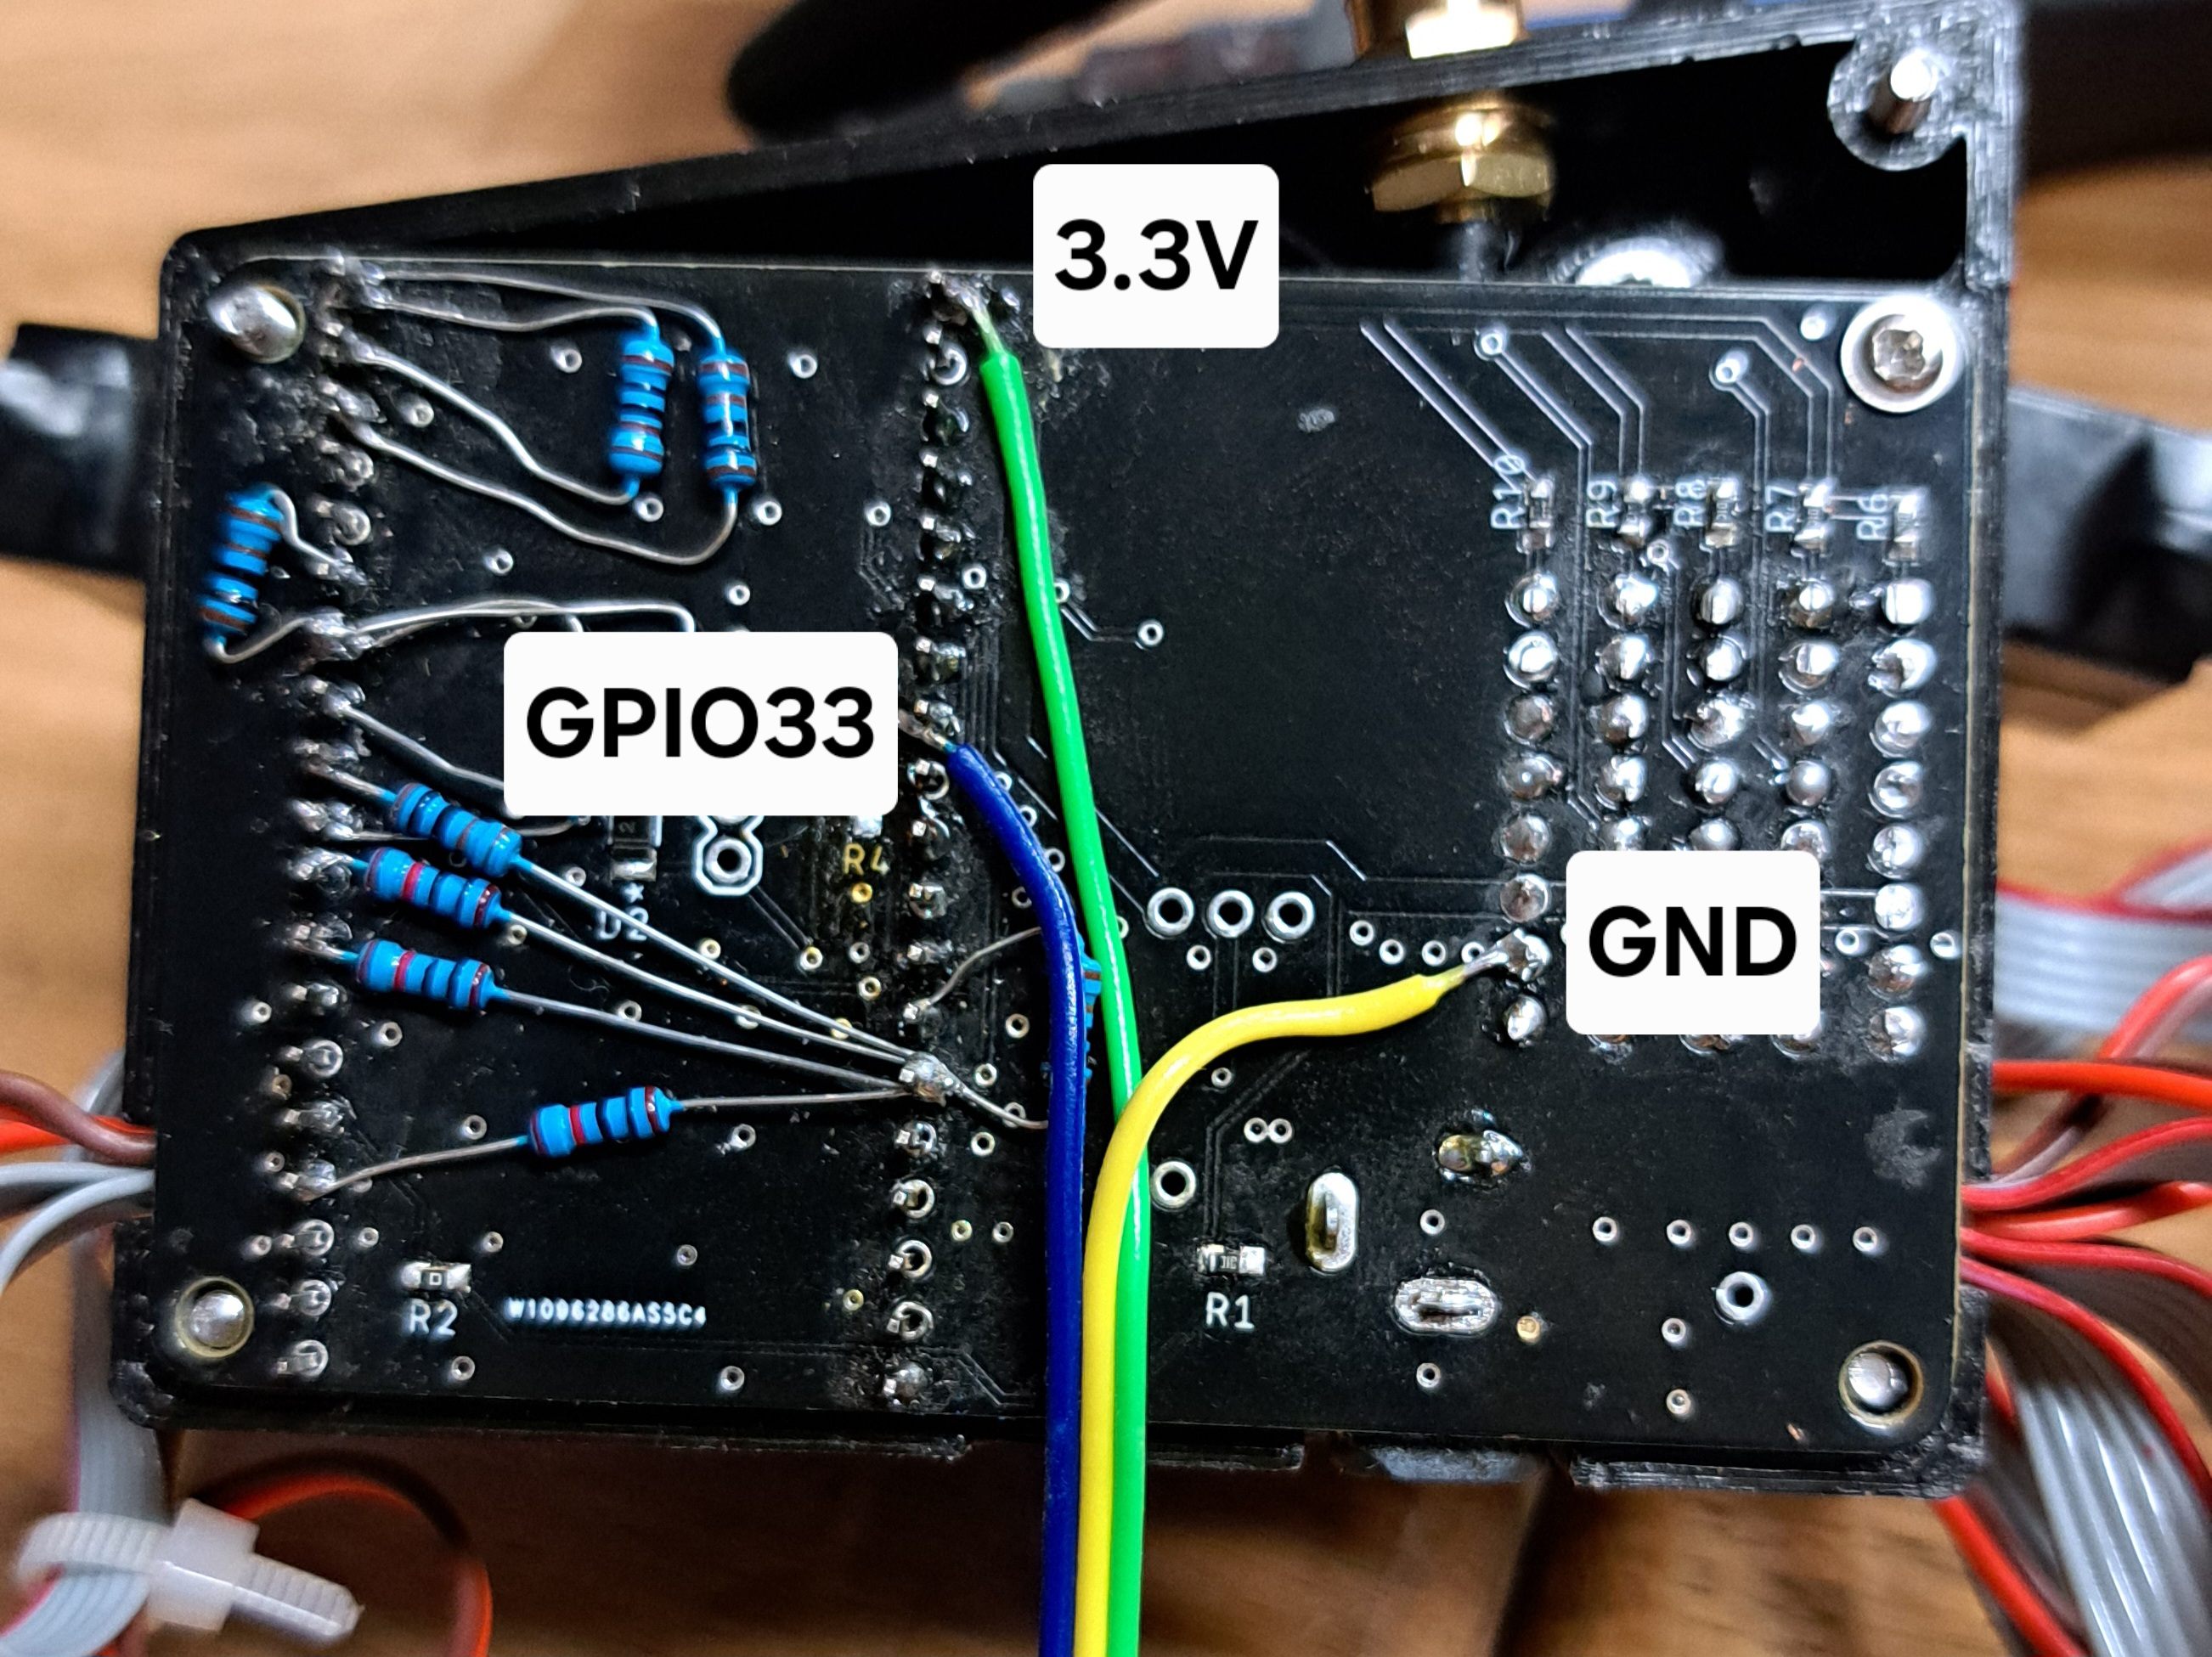
\includegraphics[width=0.6\textwidth]{Zapajeni_EMG.jpg}
\caption{Zapojení senzoru MyoWare do desky rukavice na napájení 3,3\,V, GND a vstup GPIO33.}
\label{fig:zapojeni-emg}
\end{figure}

\begin{figure}[H]
\centering
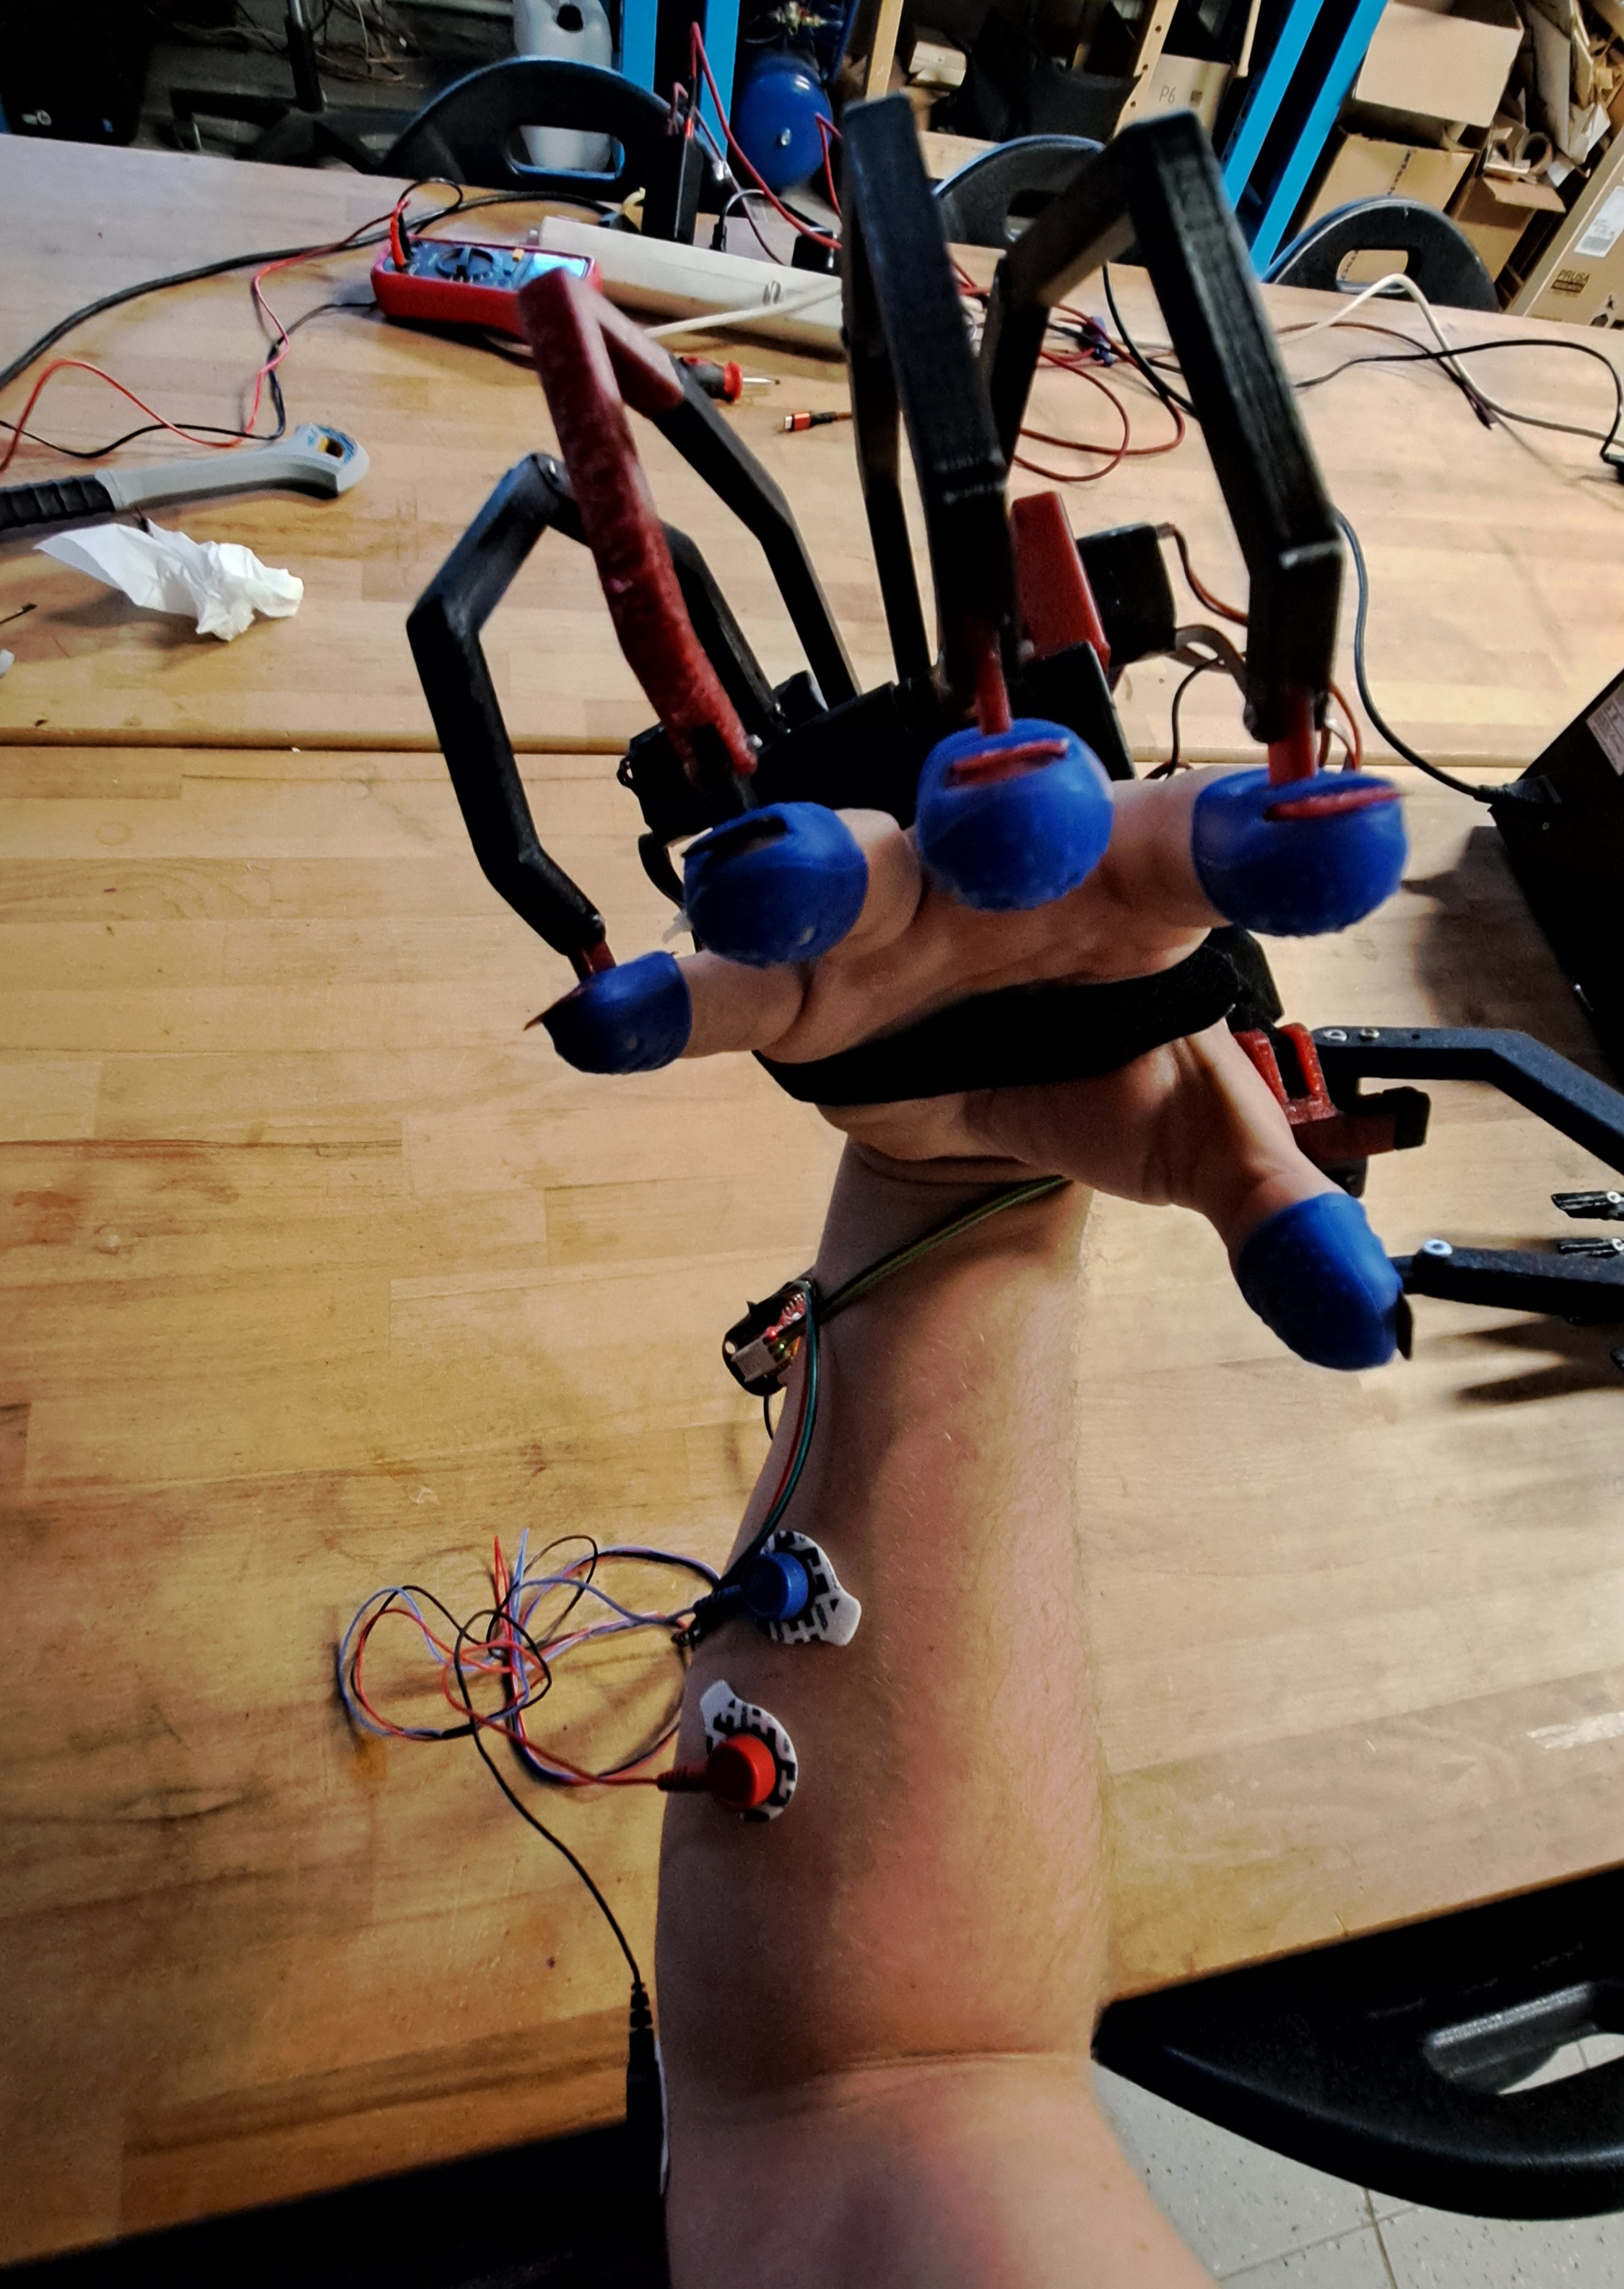
\includegraphics[width=0.4\textwidth]{Rukavice_EMG.jpg}
\caption{Nasazená rukavice Remote Feelings se senzorem MyoWare a elektrodami na předloktí.}
\label{fig:rukavice-emg}
\end{figure}

\section{Aktuační část rukavice a haptická odezva}
\label{sec:hapticka-rukavice}

Rukavice Remote Feelings byla použita jako aktivní rozhraní na straně operátora. Každý prst byl vybaven DC motorem z upraveného serva MG90S a H-můstkem A3909. Motor působil na lanko připojené k článkům prstu rukavice. Pohyb v jednom směru napomáhal zavírání prstu a pohyb v opačném směru napomáhal otevírání.

Detail konstrukce aktivní podpory jednoho prstu je uveden na obr.~\ref{fig:konstrukce-aktivni-podpory}. Obrázek ukazuje vazbu mezi upraveným servem, mechanickým držákem a prstovým táhlem rukavice.

\begin{figure}[H]
\centering
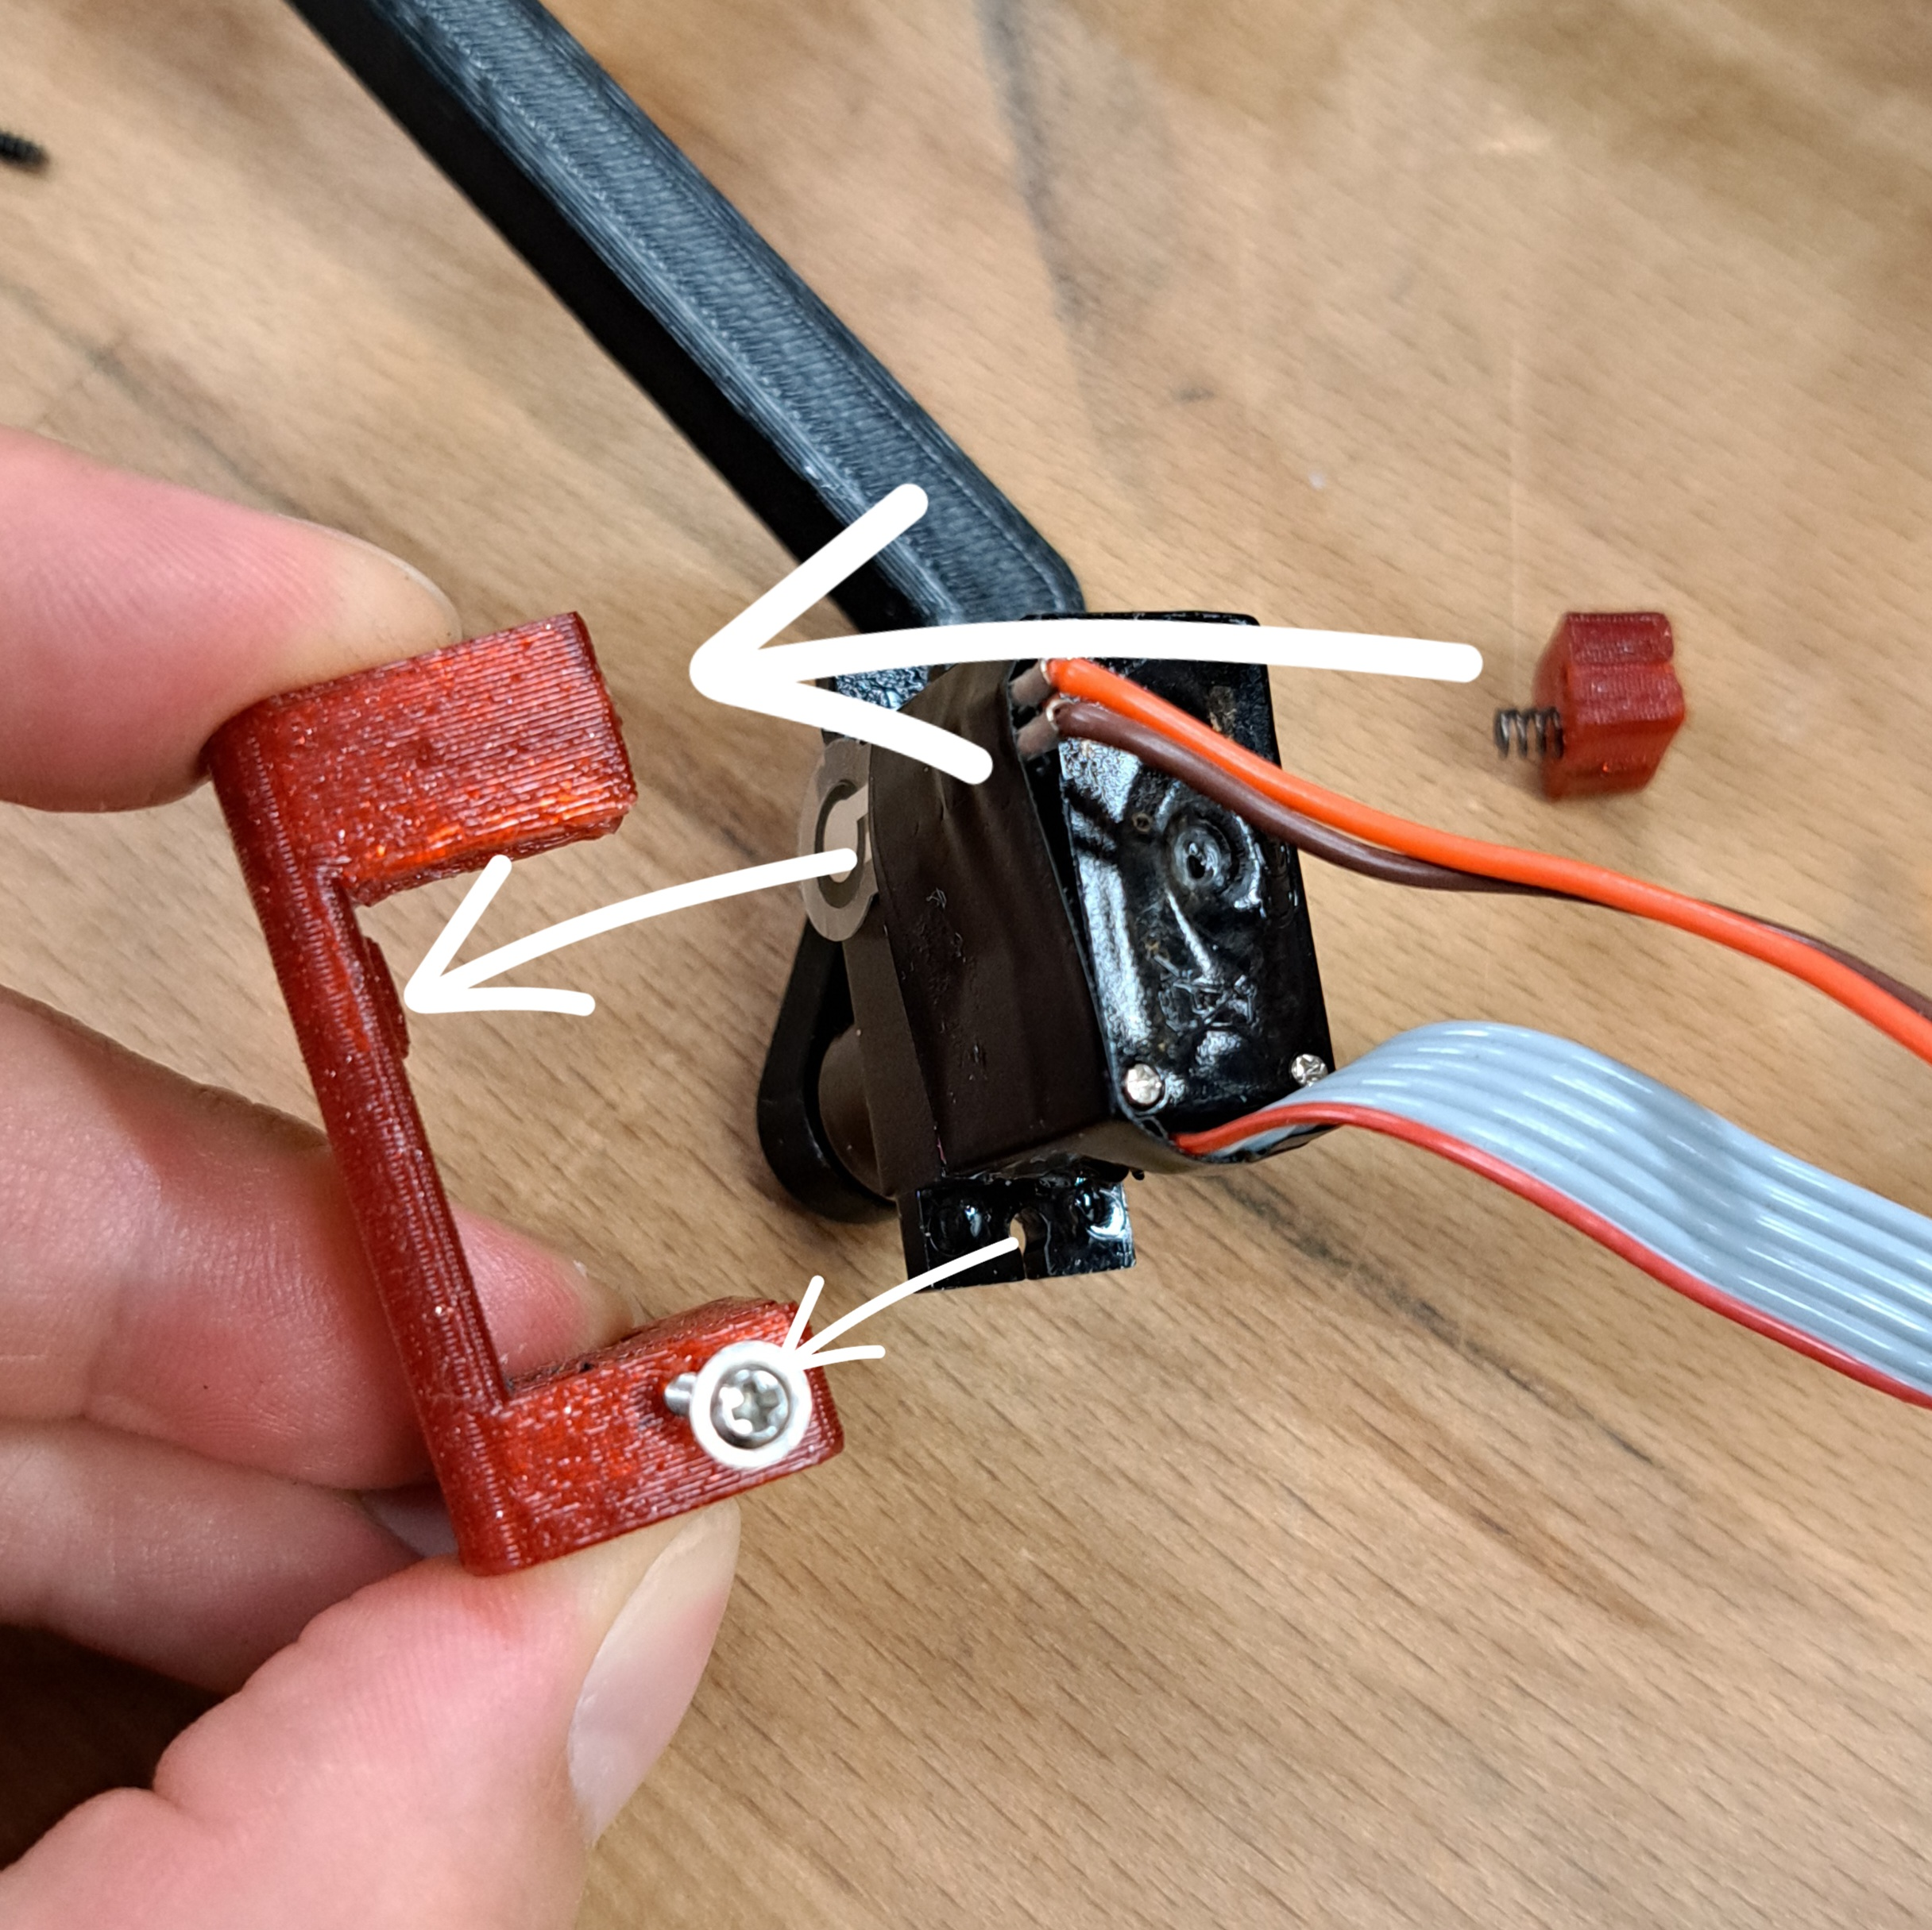
\includegraphics[width=0.6\textwidth]{konstrukce_aktivni_podpory.jpg}
\caption{Konstrukční detail aktivní podpory prstu s upraveným servem a mechanickým držákem.}
\label{fig:konstrukce-aktivni-podpory}
\end{figure}

Firmware ESP32 přiřazoval každému prstu stav asistence podle filtrované hodnoty FSR:

\begin{itemize}
    \item hodnota $+1$ označovala záměr zavírat prst,
    \item hodnota $-1$ označovala záměr otevírat prst,
    \item hodnota $0$ označovala klidový stav uvnitř mrtvého pásma.
\end{itemize}

Znaménko asistence bylo dále násobeno polaritou motoru uloženou v poli \texttt{MOTOR\_POLARITY[5]}. Tím byly kompenzovány mechanické rozdíly mezi jednotlivými prsty bez nutnosti přepojení vodičů.

Při detekci kontaktu robotického prstu s objektem byla v ESP32 aktivována haptická stěna. Aktuální poloha prstu v rukavici byla uložena jako hranice, za kterou mělo další zavírání vyvolat odpor. Pokud se uživatel pokoušel pokračovat v zavírání prstu, motor v rukavici působil proti tomuto pohybu. Otevření prstu nebo vypršení kontaktového okna haptickou stěnu zrušilo.

Mechanický princip působení aktivní podpory je ilustrován na obr.~\ref{fig:princip-aktivni-podpory}. Šipky vyznačují směr působení táhla a pohybový odpor, který uživatel vnímá při aktivaci motoru.

\begin{figure}[H]
\centering
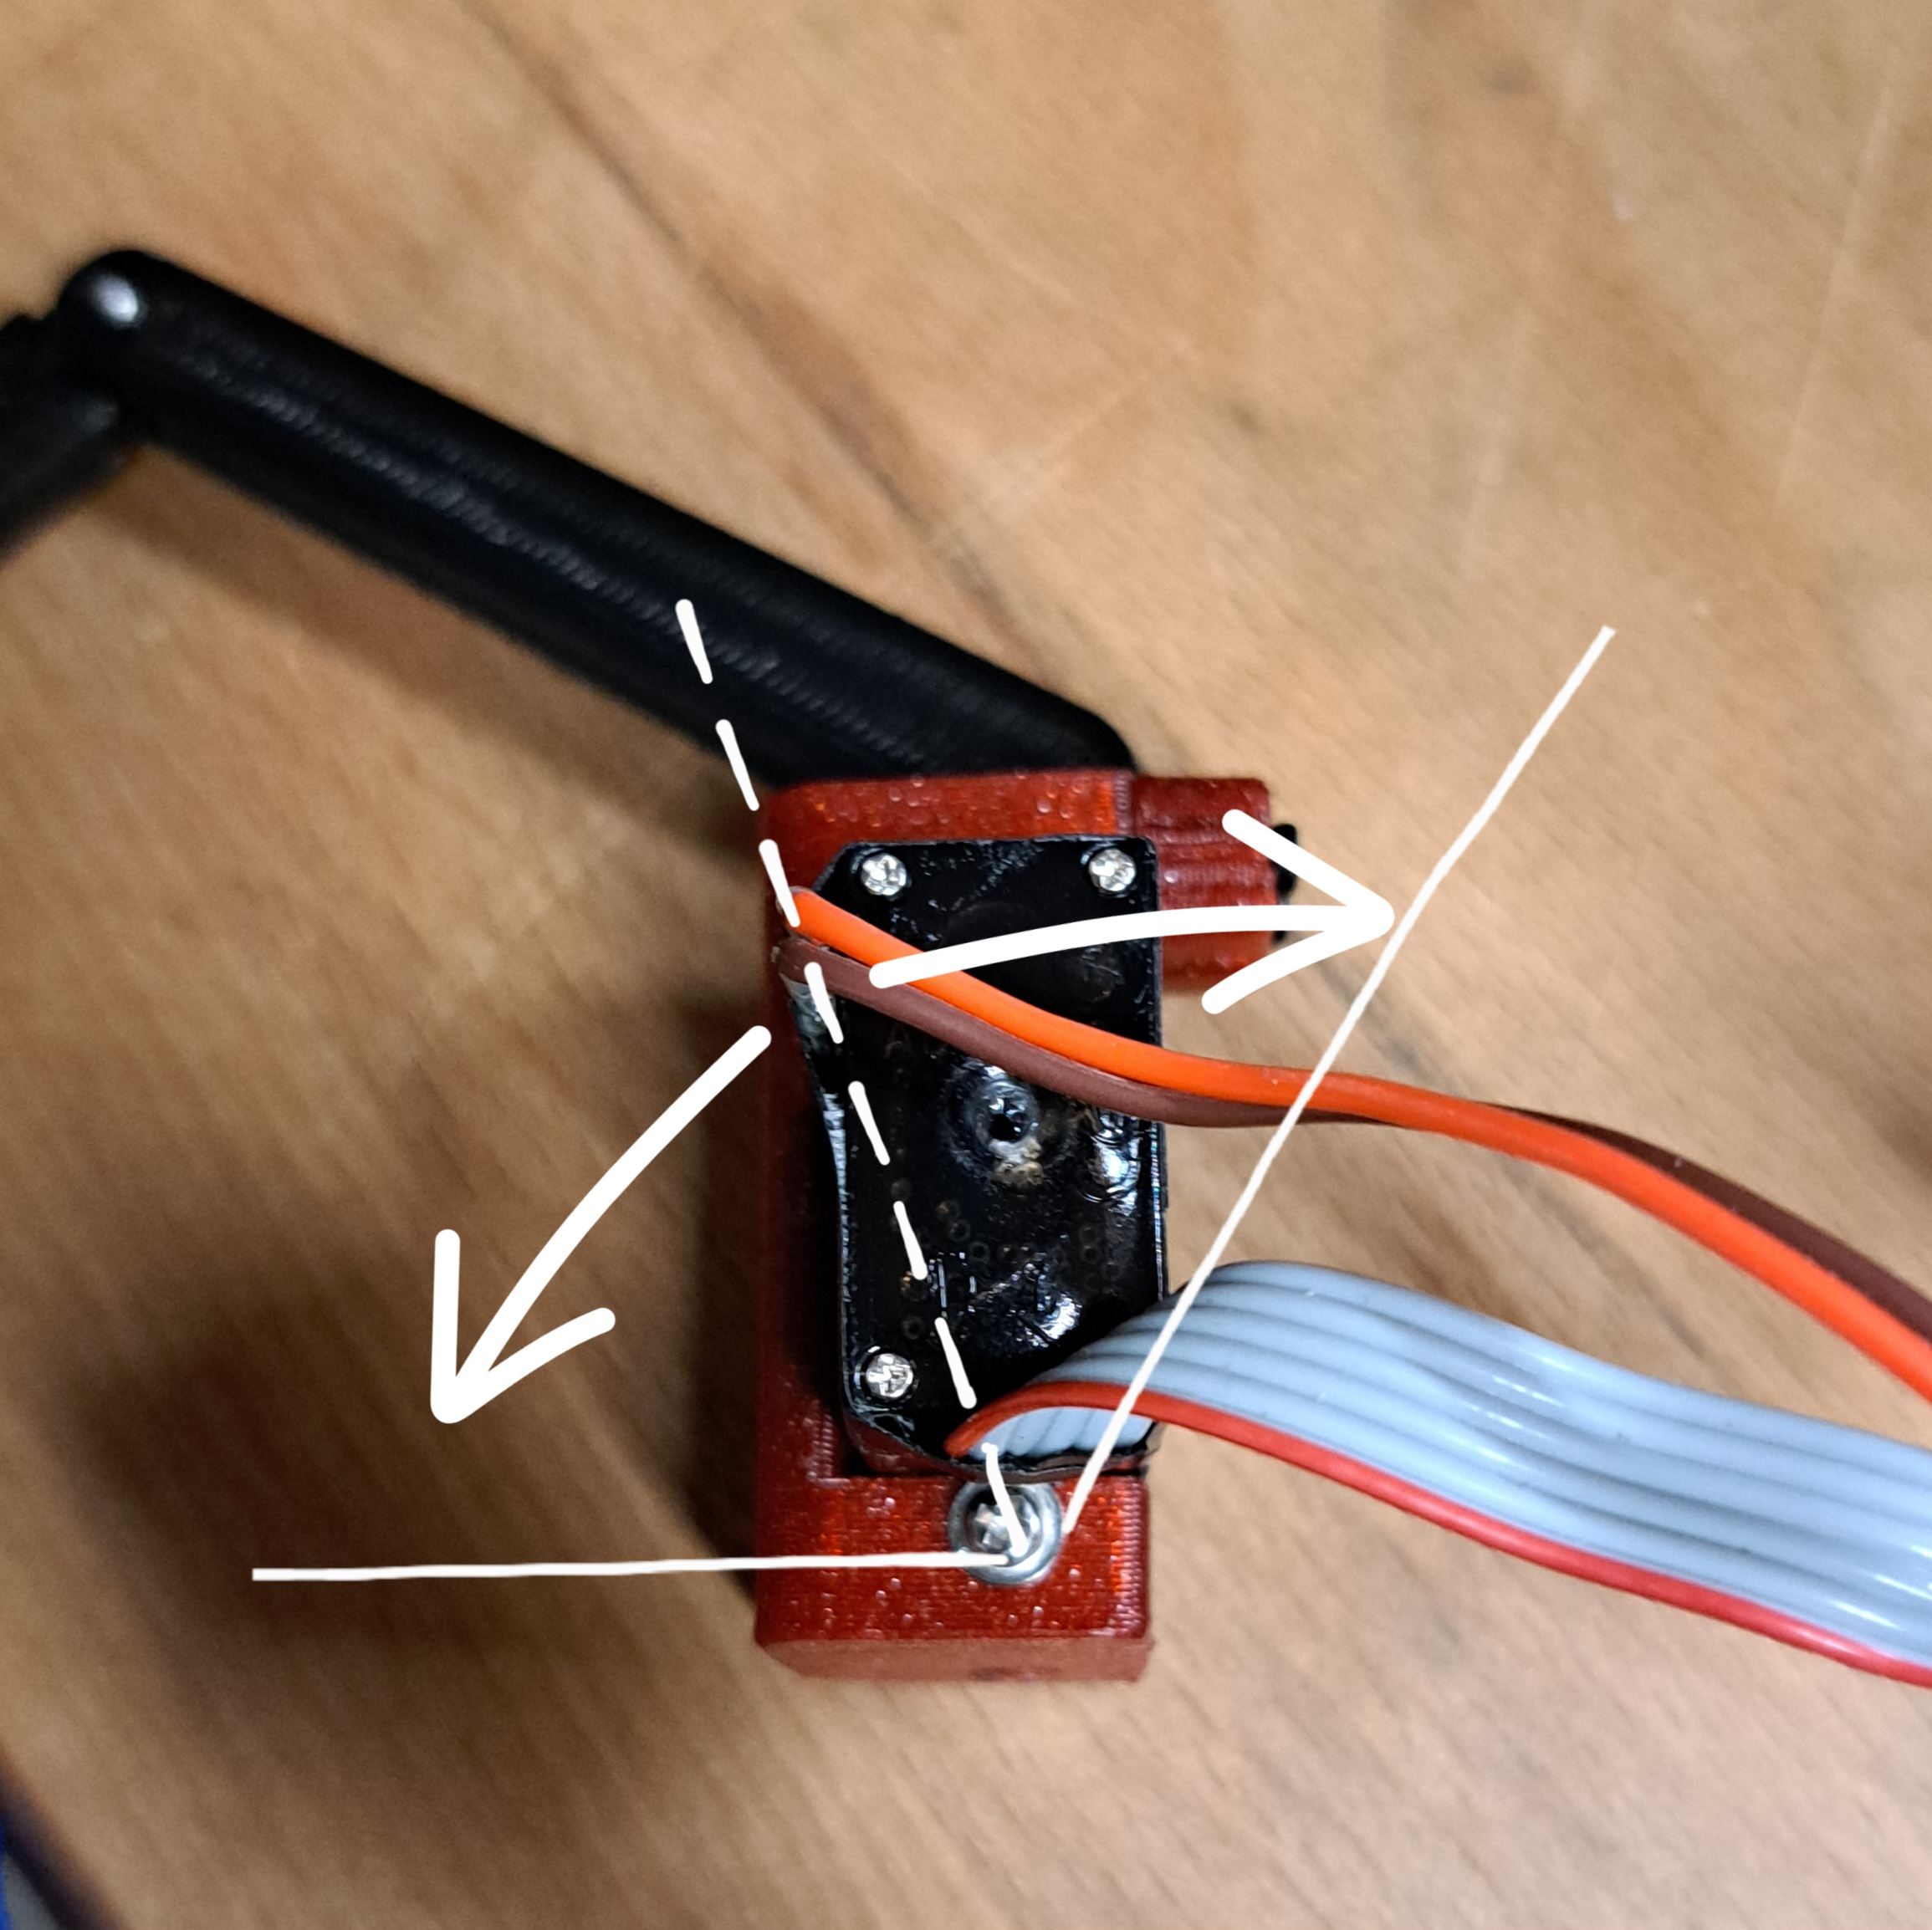
\includegraphics[width=0.6\textwidth]{Princip_aktivni_podpory.jpg}
\caption{Princip působení aktivní podpory prstu při motorickém odporu rukavice.}
\label{fig:princip-aktivni-podpory}
\end{figure}

Intenzita odporu byla odvozena z hodnoty \texttt{contactIntensity} v rozsahu 0--255. Výsledná hodnota PWM byla určena vztahem
\begin{equation}
    \mathrm{PWM} =
    \mathrm{PWM}_{\min} +
    \frac{\mathrm{intenzita}}{255}
    \left(\mathrm{PWM}_{\max} - \mathrm{PWM}_{\min}\right).
\end{equation}
Pro jednotlivé prsty byly použity minimální hodnoty PWM 250, 230, 230, 250 a 250 a maximální hodnoty 650, 550, 550, 650 a 650 z rozsahu 0--1023. Haptický odpor byl tímto způsobem omezen na předem nastavený bezpečný rozsah.

\section{Robotická ruka InMoov a řídicí elektronika}
\label{sec:roboticka-ruka}

Robotická ruka InMoov byla použita jako 3D tisknutelná open-source robotická ruka s lankovým převodem pohybu prstů \cite{InMoov}. Každý prst byl ovládán jedním servomotorem MG996R umístěným v předloktí. Řídicí jednotkou byla deska Arduino UNO s mikrokontrolérem ATmega328P.

\subsection{Servomotory MG996R}
\label{subsec:mg996r}

Každý prst robotické ruky byl ovládán servomotorem MG996R s kovovými převody. Podle technických údajů dosahuje servo momentu 9,4\,kg$\cdot$cm při 4,8\,V a 11\,kg$\cdot$cm při 6\,V. Proud při zablokovaném motoru je uváděn přibližně 2,5\,A při 6\,V \cite{mg996r_towerpro}. Při současném záběru pěti serv by proto mohl okamžitý proud překročit 12\,A.

Servomotory proto nebyly napájeny z USB ani z pinu 5\,V desky Arduino UNO\@. Byl použit samostatný výkonový zdroj 5--6\,V se společnou zemí s řídicí elektronikou. Pro opakovatelný provoz byla uvažována proudová rezerva 10--15\,A. K napájecí sběrnici byl doplněn elektrolytický kondenzátor 1000\,$\mu$F / 16\,V pro potlačení krátkých proudových špiček.

Řízení serv bylo ve finální implementaci provedeno standardní knihovnou \texttt{Servo.h}. Modul HC-05 byl připojen na hardwarový UART D0/D1, takže nebyla použita knihovna \texttt{SoftwareSerial}. Tím byl odstraněn konflikt mezi softwarovou sériovou linkou a přesným časováním řídicích pulzů serv. Nevýhodou tohoto zapojení byla nutnost odpojit HC-05 při nahrávání firmware.

\subsection{Senzory proudu INA219}
\label{subsec:ina219}

Proudový odběr každého servomotoru byl měřen modulem INA219. Pět modulů bylo zapojeno paralelně na I2C sběrnici Arduino UNO, kde SDA odpovídá pinu A4 a SCL pinu A5 \cite{Lebosse2011,ti_ina219}. Senzor INA219 měří úbytek napětí na bočníku ($V_{\mathrm{sh}}$) a napětí
na sběrnici. Proud je z naměřeného úbytku napětí odvozen interně na základě
Ohmova zákona:

$$I = \frac{V_{shunt}}{R_{shunt}}$$

Aby čip věděl, jaký odpor bočníku je použit, je nutné před měřením zapsat
do kalibračního registru hodnotu $CAL$:

$$CAL = \frac{0{,}04096}{I_{LSB} \cdot R_{shunt}}$$

kde $0{,}04096$ je pevná konstanta čipu, $I_{LSB}$ je požadované rozlišení
proudu na jeden bit (např. $0{,}1\ \mathrm{mA}$) a $R_{shunt}$ je odpor
bočníku (např. $0{,}1\ \Omega$). Na základě této hodnoty čip interně
vypočítá proud:

$$I = \frac{V_{\mathrm{sh}} \cdot CAL}{4096}$$

kde $V_{\mathrm{sh}}$ je naměřená hodnota z registru úbytku napětí.
Výsledný proud je pak dostupný přímo ke čtení z interního registru v~mA.

V použité knihovně byla využívána funkce \texttt{getCurrent\_mA()}.

Každý modul musel mít nastavenu odlišnou I2C adresu. Použitá konfigurace je uvedena v tabulce~\ref{tab:ina219}.

\begin{table}[H]
\centering
\caption{I2C adresy modulů INA219 podle prstu robotické ruky}
\label{tab:ina219}
\begin{tabular}{|p{0.25\textwidth}|p{0.25\textwidth}|p{0.30\textwidth}|}
\hline
\textbf{Prst} & \textbf{I2C adresa} & \textbf{Konfigurace A0 / A1} \\
\hline
Palec & \texttt{0x40} & GND / GND \\
\hline
Ukazovák & \texttt{0x41} & VCC / GND \\
\hline
Prostředník & \texttt{0x44} & GND / VCC \\
\hline
Prsteník & \texttt{0x45} & VCC / VCC \\
\hline
Malíček & \texttt{0x48} & GND / SDA \\
\hline
\end{tabular}
\end{table}

Adresování modulů INA219 bylo provedeno pájením adresových propojek na deskách senzorů. Čtyři použité konfigurace jsou ukázány na obr.~\ref{fig:ina219-4x}; detail páté konfigurace modulu je uveden na obr.~\ref{fig:ina219-1x}.

\begin{figure}[H]
\centering
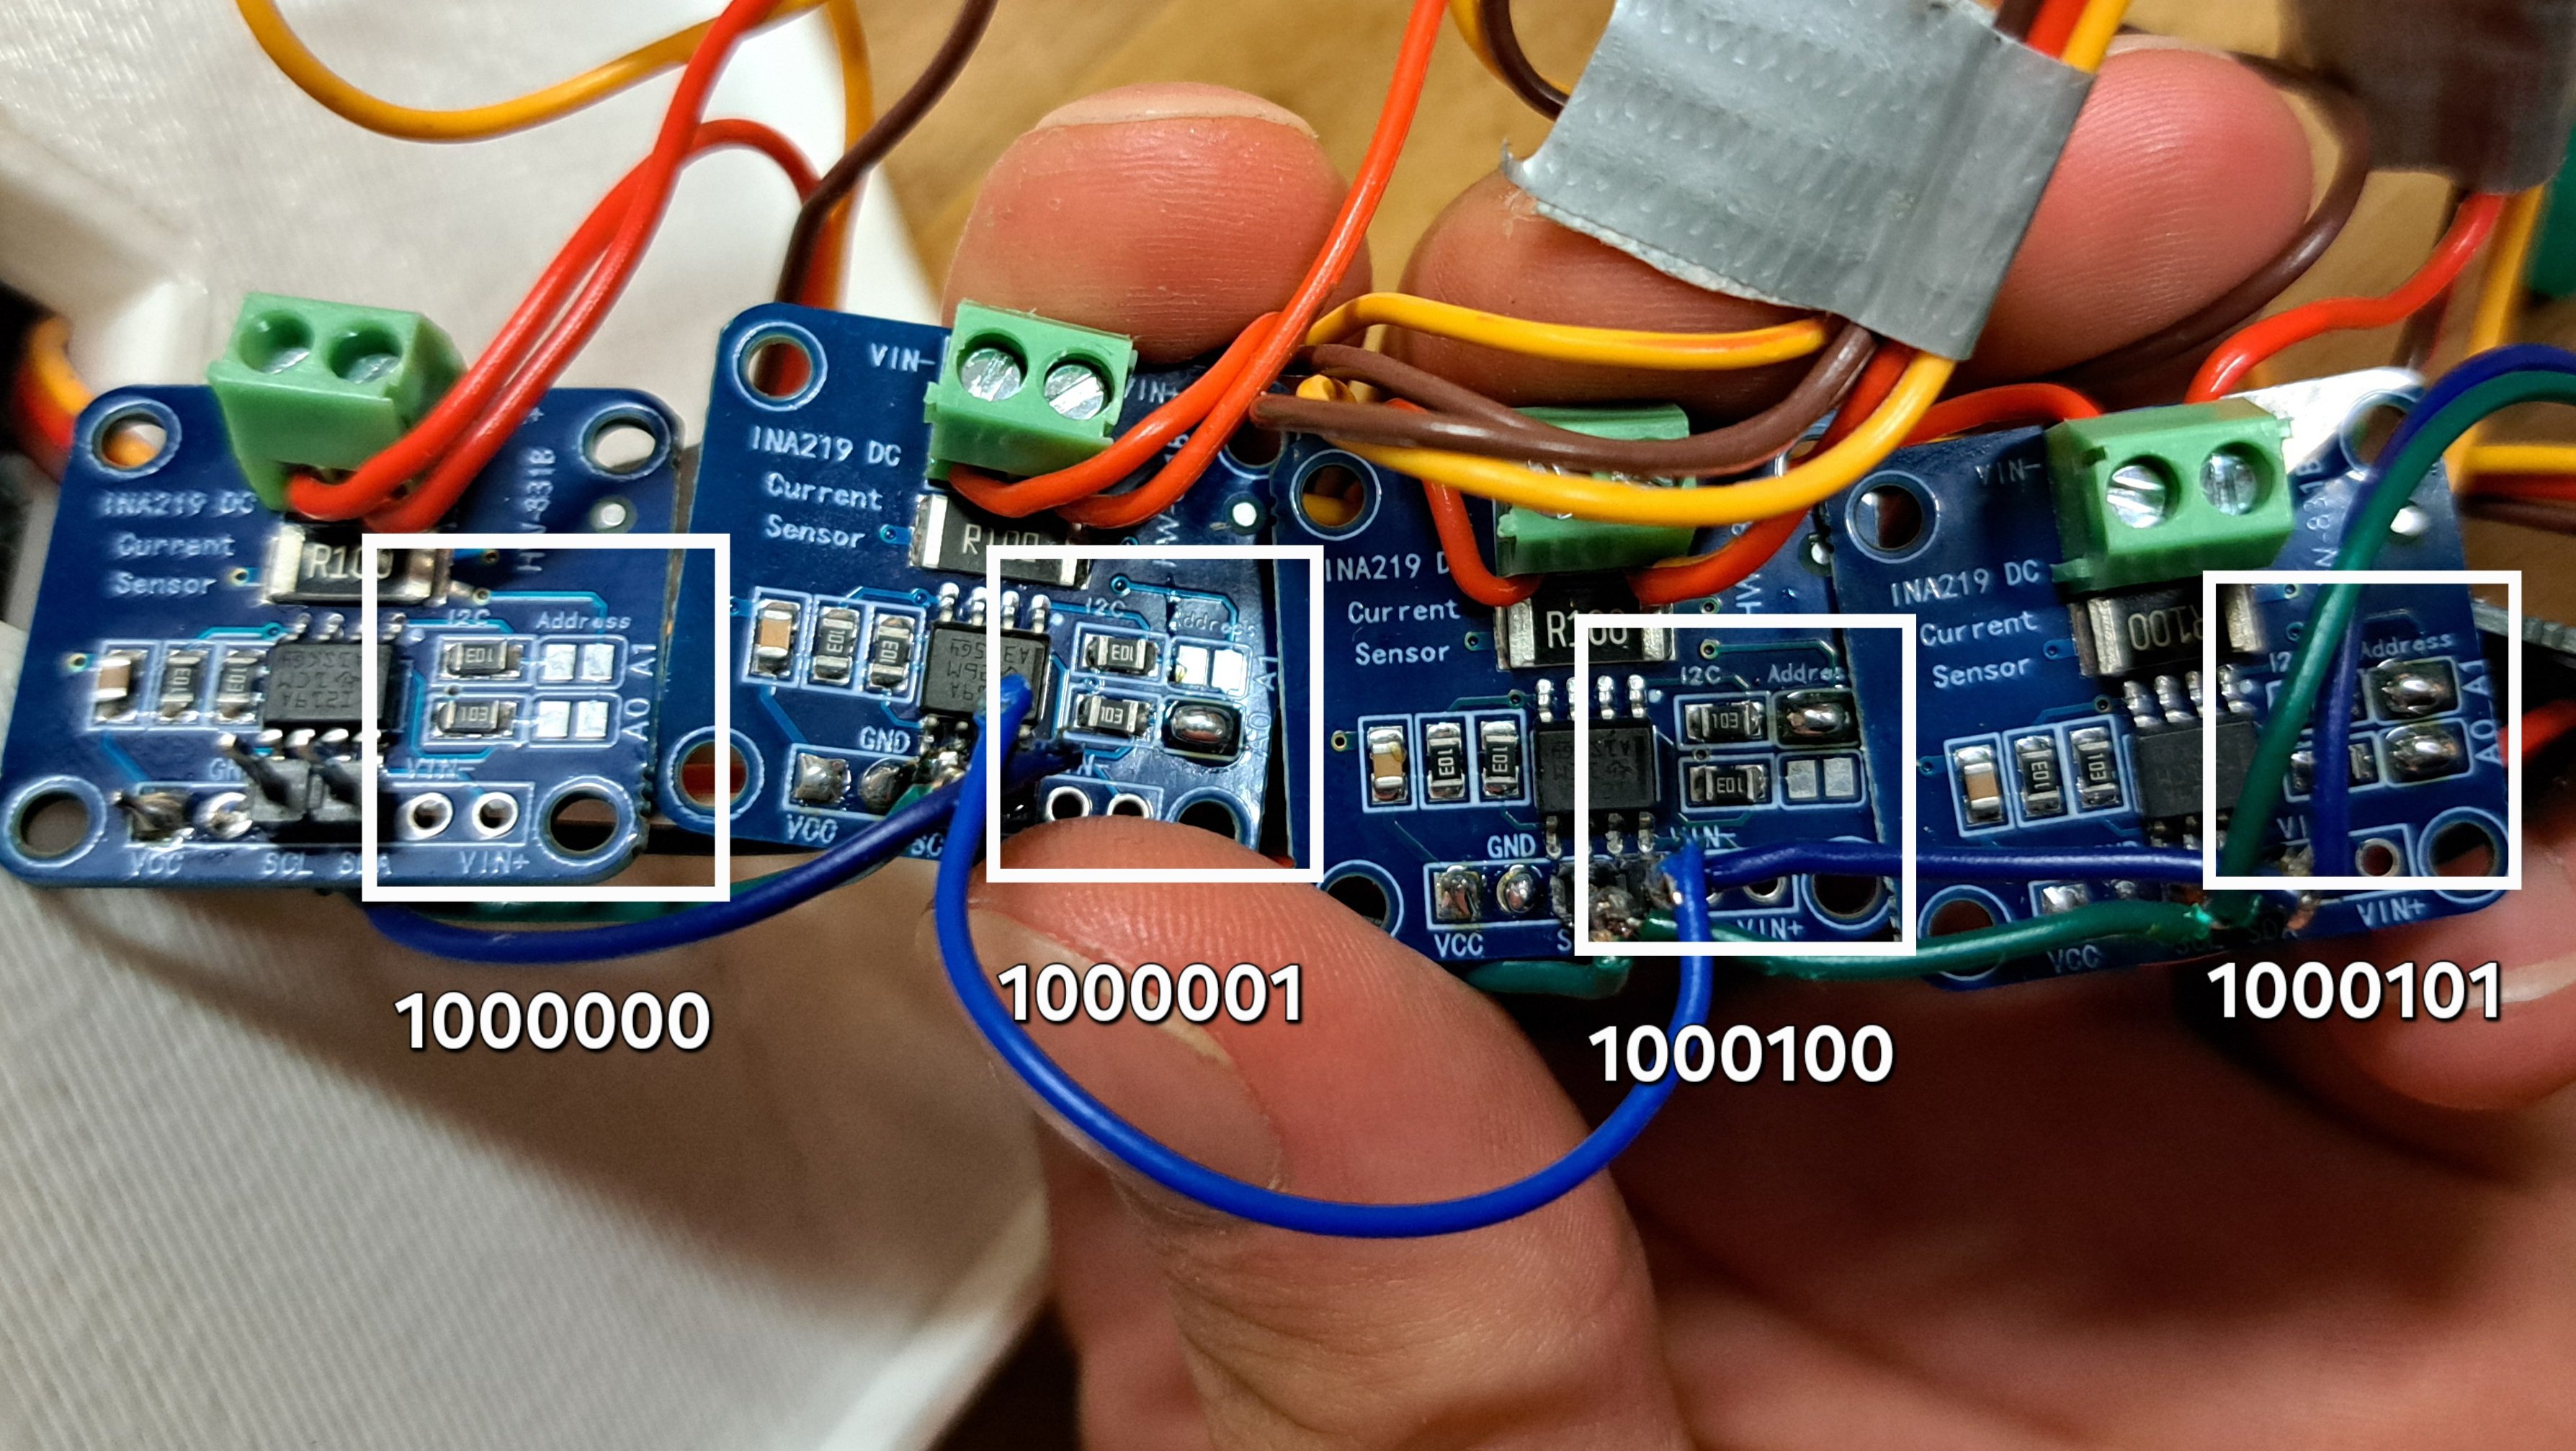
\includegraphics[width=0.95\textwidth]{INA219_4x.jpg}
\caption{Čtyři moduly INA219 s odlišně nastavenými adresovými propojkami na I2C sběrnici.}
\label{fig:ina219-4x}
\end{figure}

\begin{figure}[H]
\centering
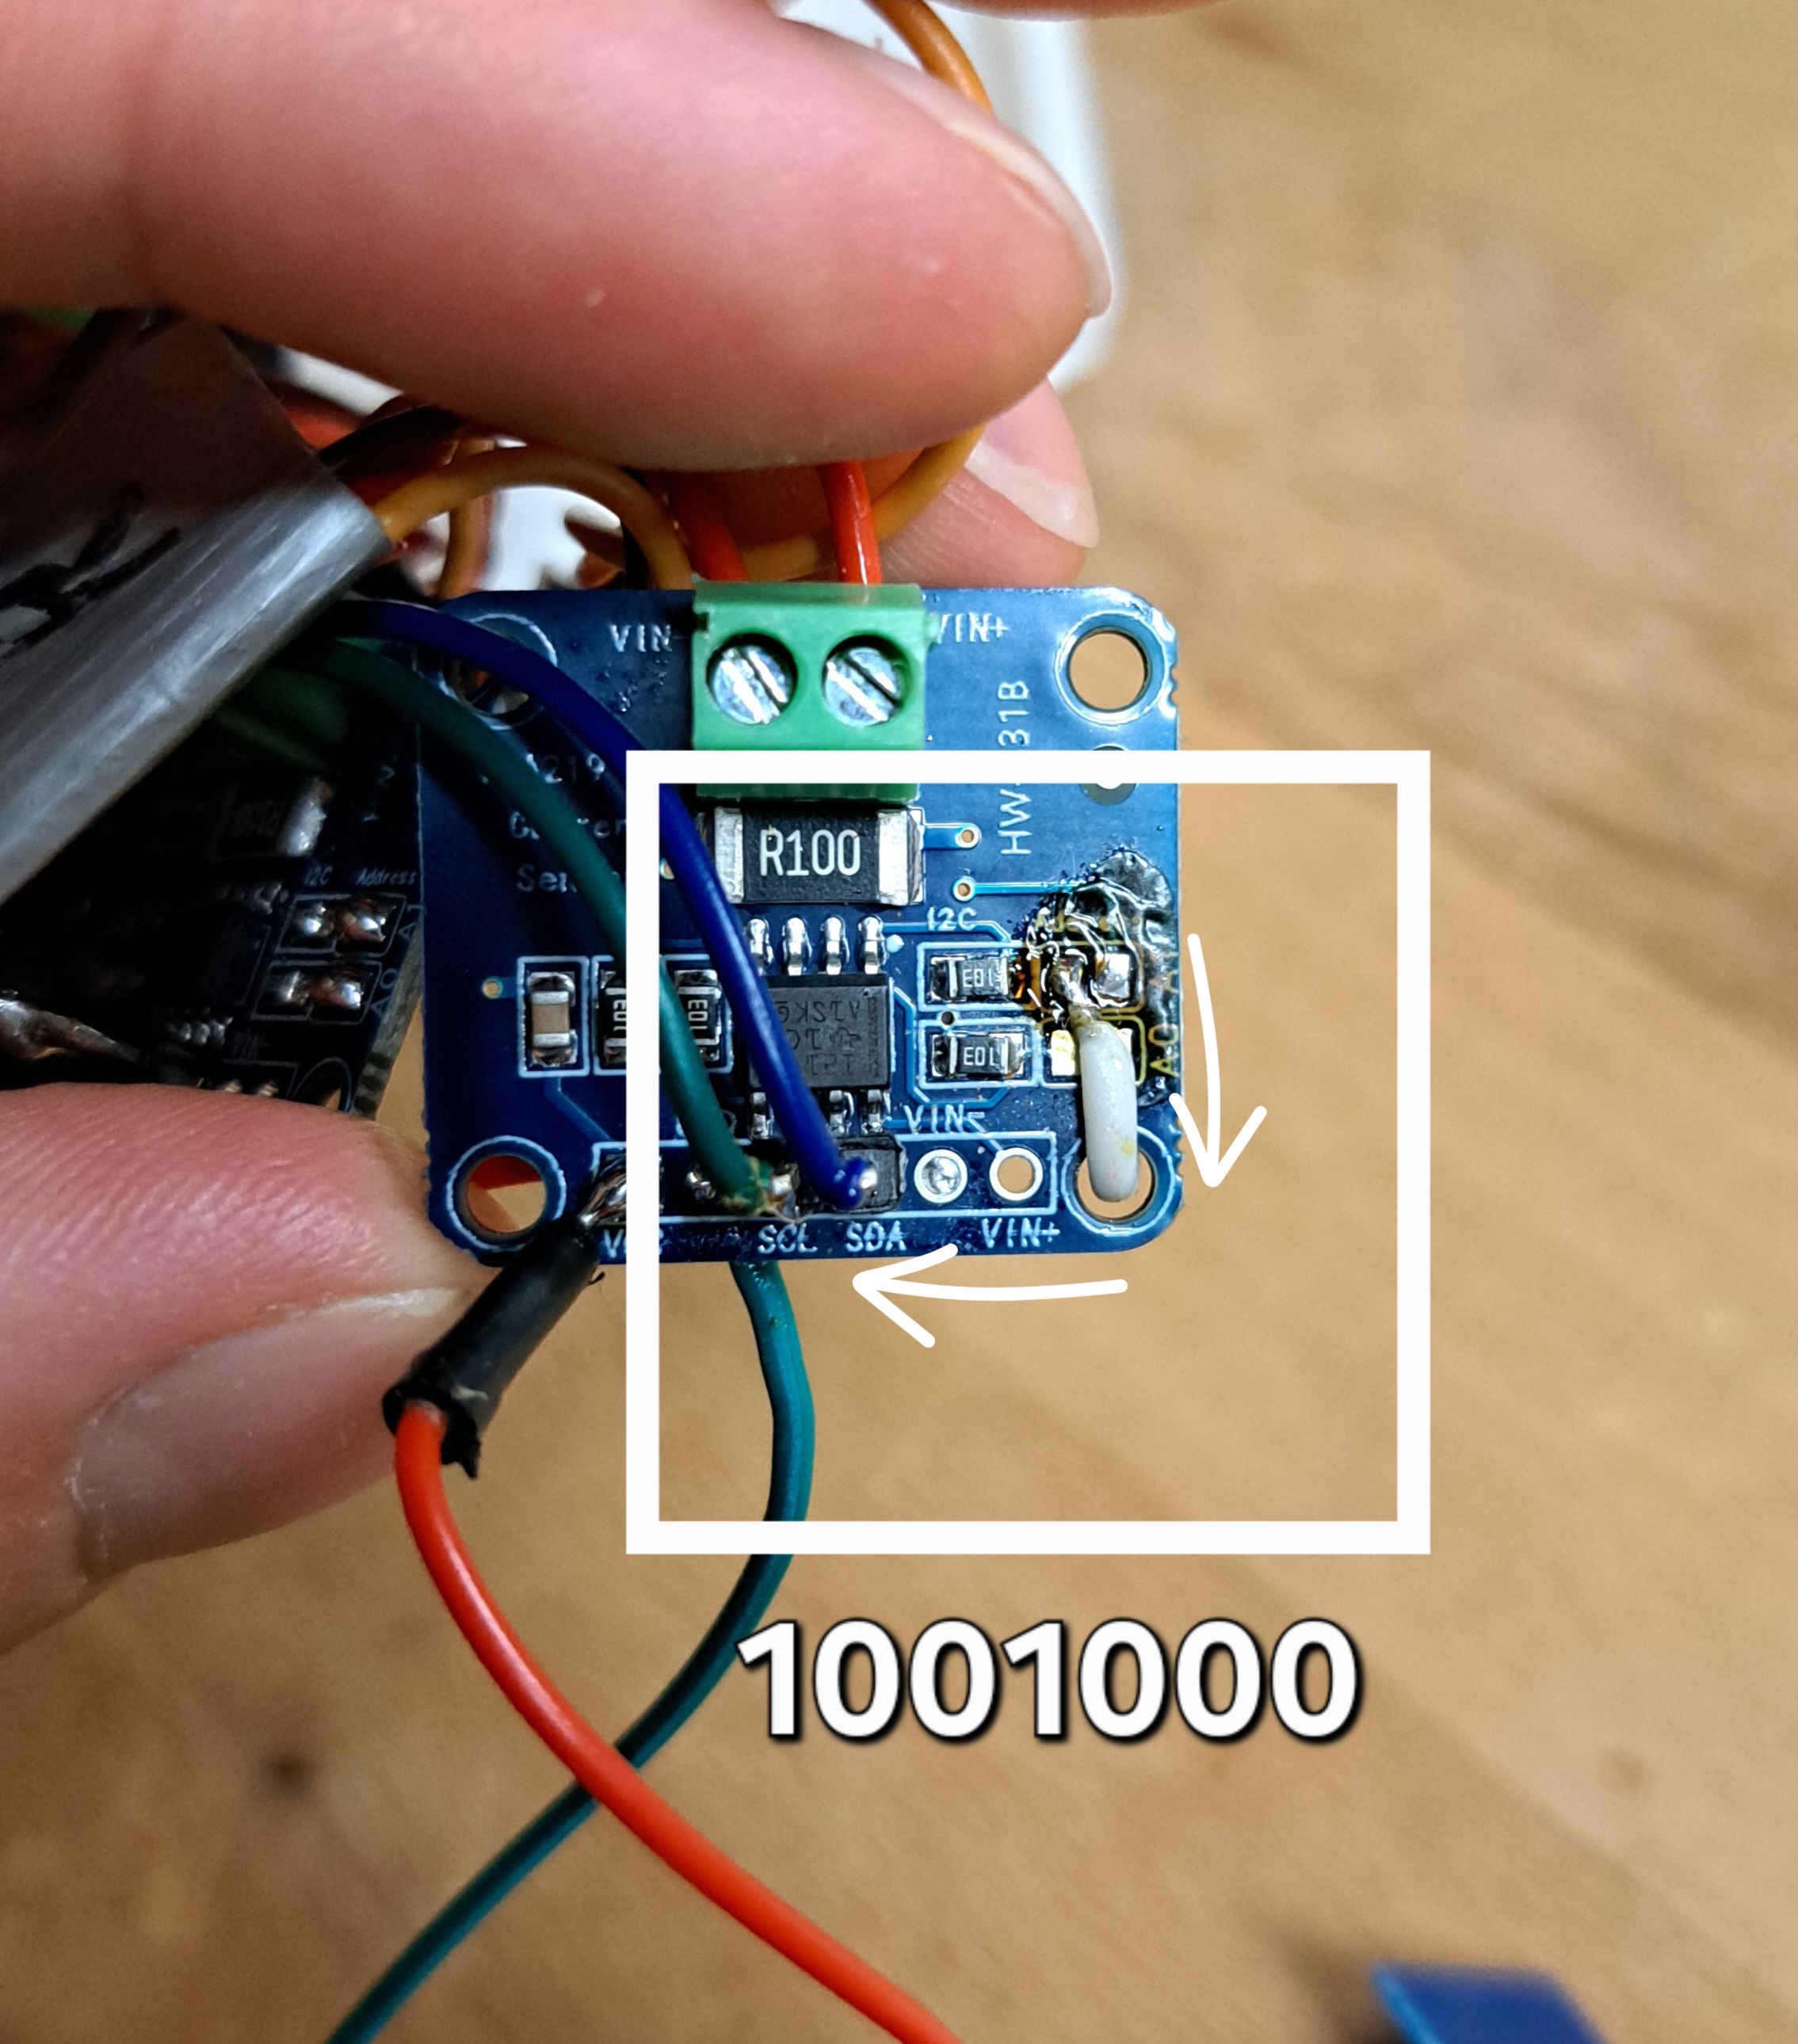
\includegraphics[width=0.52\textwidth]{INA219_1x.jpg}
\caption{Detail adresové konfigurace jednoho modulu INA219.}
\label{fig:ina219-1x}
\end{figure}

\subsection{Bluetooth modul HC-05 a přizpůsobení úrovní}
\label{subsec:hc05}

Bezdrátové spojení bylo realizováno modulem HC-05 v roli Bluetooth Slave \cite{Sadun2016711}. Modul byl napájen z 5\,V pinu Arduino UNO a komunikoval rychlostí 9600 Bd. Po úspěšném spárování přenášel data jako transparentní sériová linka.

Protože logické úrovně vstupu HC-05 jsou 3,3\,V a výstup Arduino UNO má úroveň 5\,V, byl na lince Arduino TX $\rightarrow$ HC-05 RX použit odporový dělič napětí
\begin{equation}
    V_{\mathrm{out}} = V_{\mathrm{in}} \frac{R_2}{R_1 + R_2}
    = 5\,\mathrm{V}\frac{2\,\mathrm{k}\Omega}{1\,\mathrm{k}\Omega + 2\,\mathrm{k}\Omega}
    = 3{,}33\,\mathrm{V}.
\end{equation}

Praktické zapojení odporového děliče na nepájivém poli je znázorněno na obr.~\ref{fig:napetovy-delic}. Dělič byl vložen do směru Arduino TX $\rightarrow$ HC-05 RXD.

\begin{figure}[H]
\centering
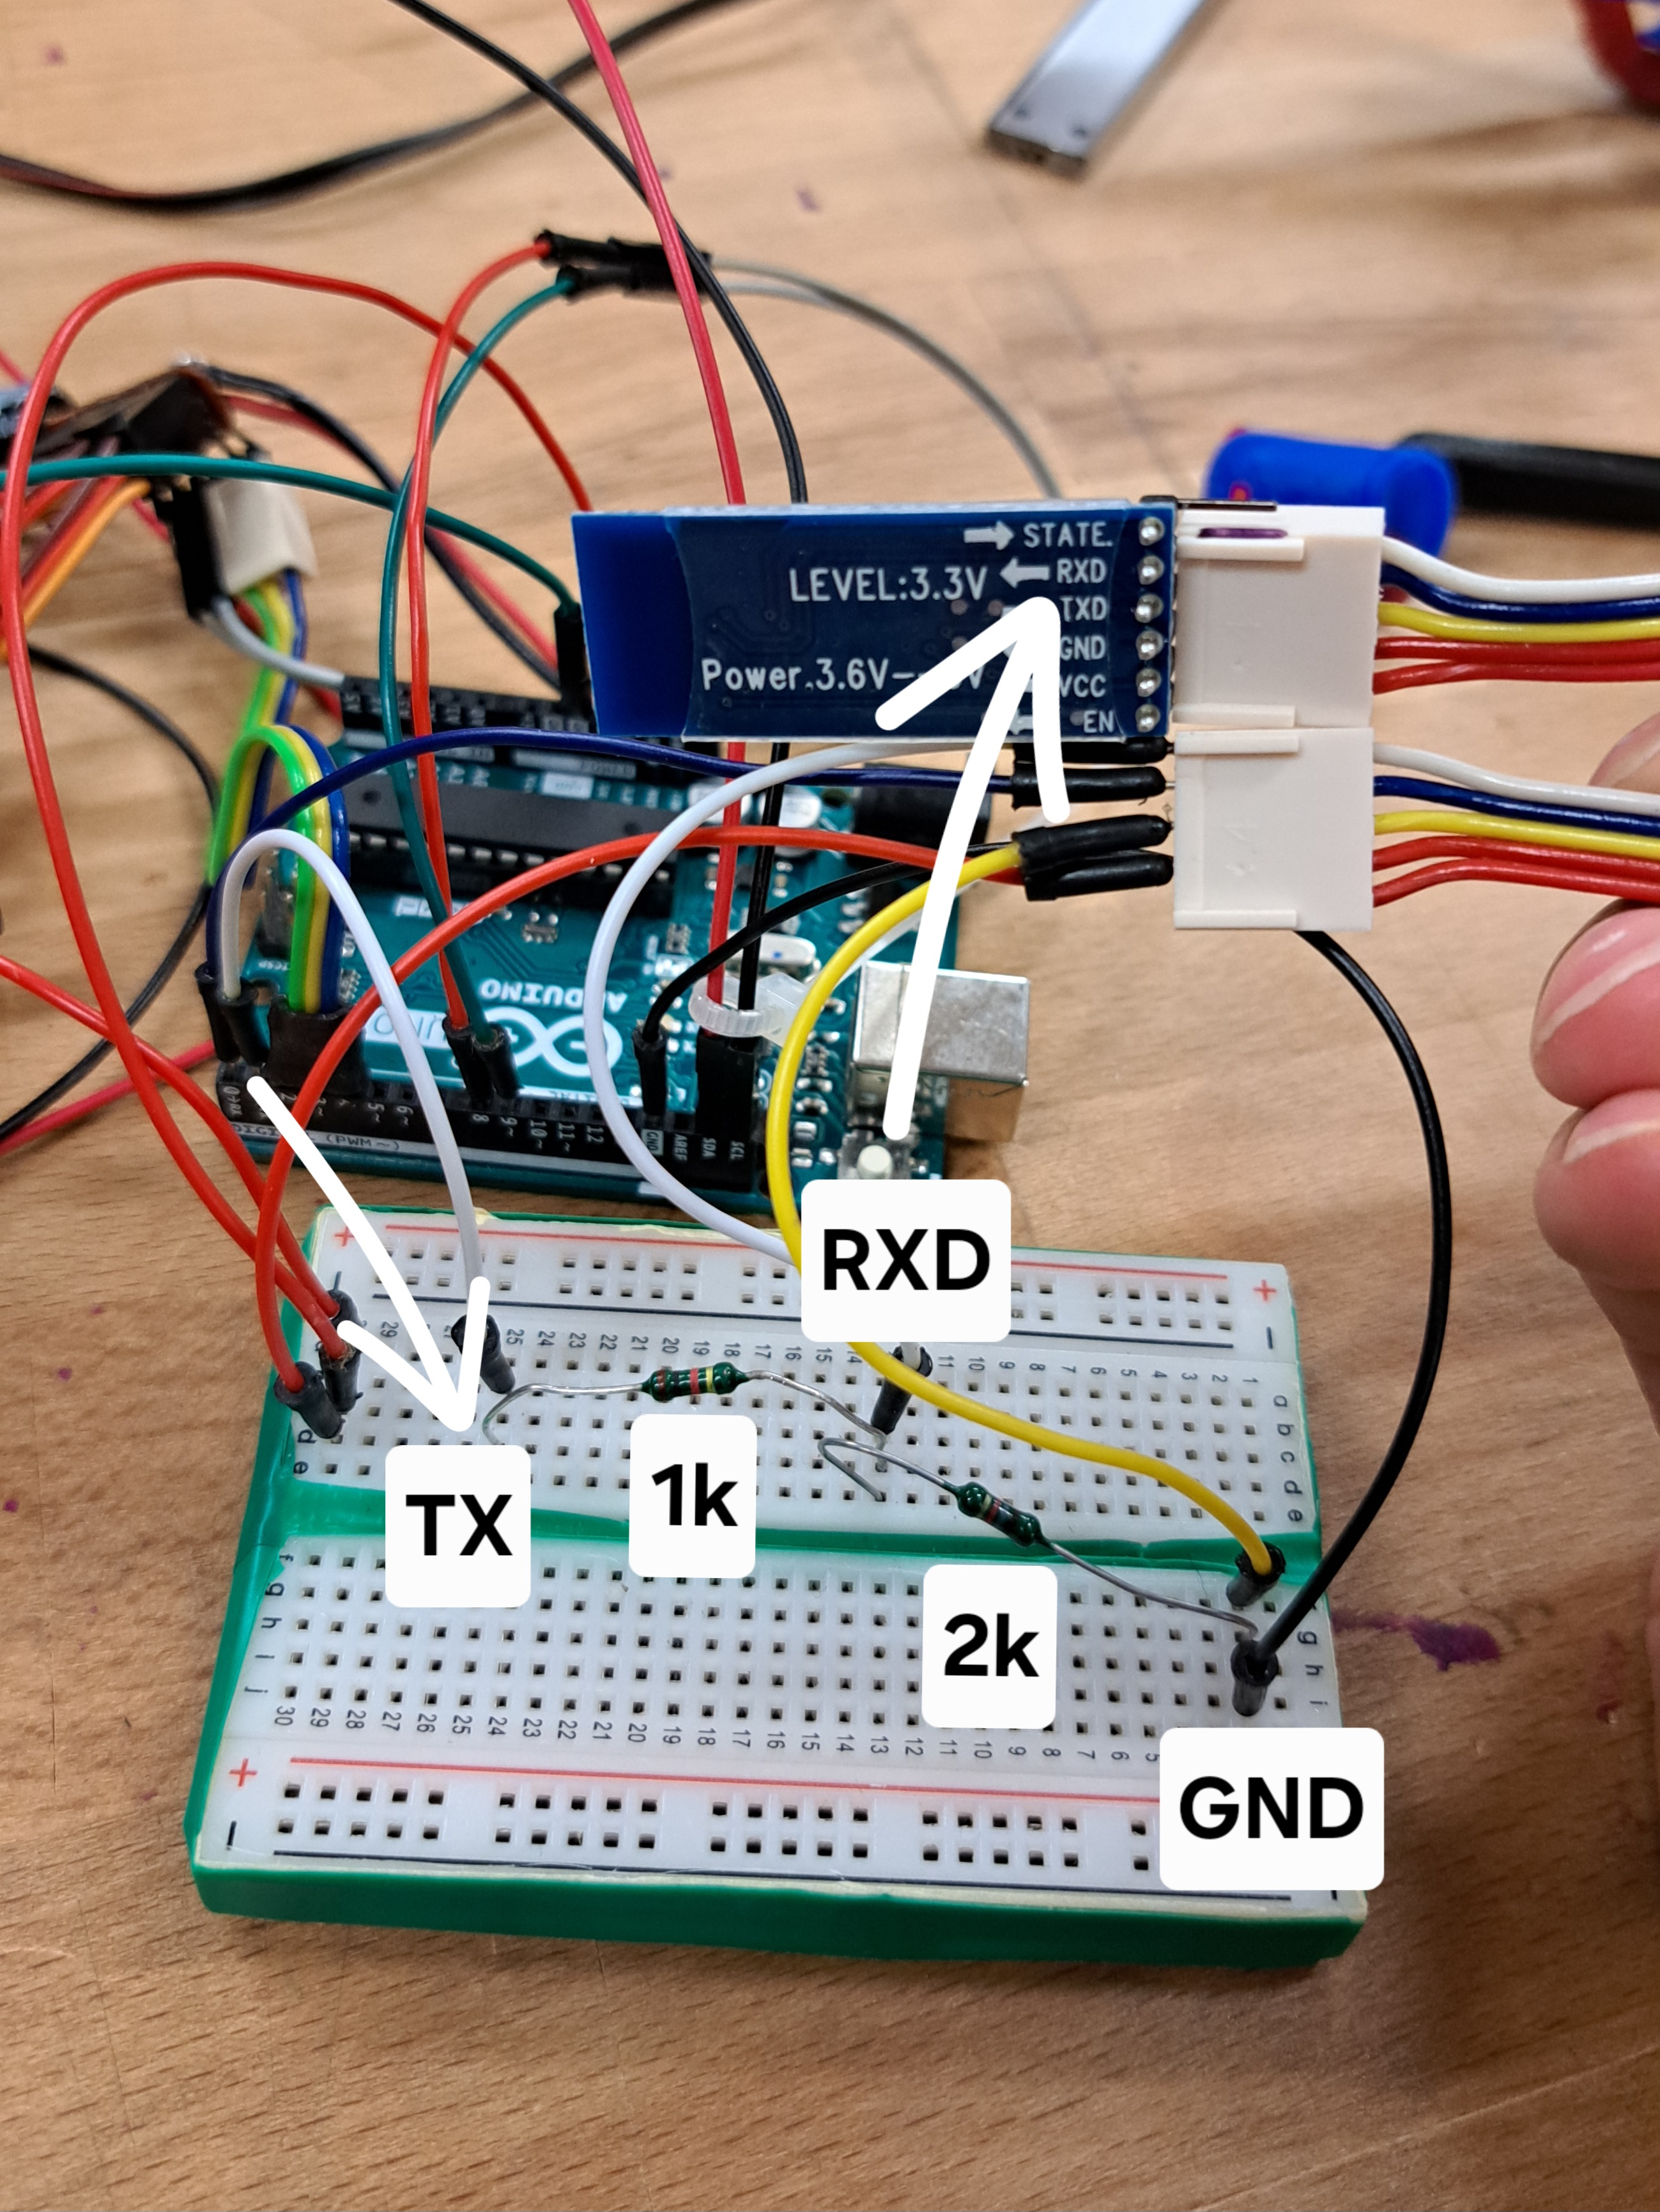
\includegraphics[width=0.52\textwidth]{napetovy_delic.jpg}
\caption{Odporový dělič 1\,k$\Omega$ / 2\,k$\Omega$ pro přizpůsobení úrovně signálu Arduino TX na vstup HC-05 RXD.}
\label{fig:napetovy-delic}
\end{figure}
Opačný směr HC-05 TX $\rightarrow$ Arduino RX nevyžadoval dělič, protože napětí 3,3\,V bylo Arduino UNO spolehlivě rozpoznáno jako logická úroveň HIGH.

\section{Komunikační rozhraní a struktura paketů}
\label{sec:komunikacni-rozhrani}

Komunikace mezi ESP32 a Arduino UNO byla realizována přes Bluetooth Classic SPP\@. Na straně Arduino UNO byl modul HC-05 připojen k hardwarovému UARTu rychlostí 9600 Bd \cite{hc05_components101}. Na aplikační úrovni nebyly přenášeny textové příkazy, ale binární struktury opatřené dvojicí synchronizačních bajtů.

Paket odesílaný z ESP32 do Arduino UNO je popsán v tabulce~\ref{tab:packet-esp-uno}.

\begin{table}[H]
\centering
\caption{Paket ESP32 $\rightarrow$ Arduino UNO}
\label{tab:packet-esp-uno}
\begin{tabular}{|p{0.28\textwidth}|p{0.18\textwidth}|p{0.13\textwidth}|p{0.31\textwidth}|}
\hline
\textbf{Pole} & \textbf{Typ} & \textbf{Jednotka} & \textbf{Význam} \\
\hline
\texttt{start1}, \texttt{start2} & 2$\times$ \texttt{uint8\_t} & -- & Synchronizace paketu; hodnoty \texttt{0xAA} a \texttt{0xBB}. \\
\hline
\texttt{servoAngles[5]} & 5$\times$ \texttt{uint8\_t} & $^\circ$ & Cílové logické úhly serv v režimu MIRROR\@. \\
\hline
\texttt{emgRaw} & \texttt{uint16\_t} & ADC & Surová hodnota sEMG z ESP32. \\
\hline
\texttt{emgMin}, \texttt{emgMax}, \texttt{emgThreshold} & 3$\times$ \texttt{float} & ADC & Kalibrační hodnoty pro režim EMG\@. \\
\hline
\texttt{calibrated} & \texttt{uint8\_t} & -- & Příznak platné kalibrace. \\
\hline
\texttt{forceFeedbackEnabled} & \texttt{uint8\_t} & -- & Povolení kontaktní detekce a haptiky. \\
\hline
\texttt{controlMode} & \texttt{uint8\_t} & -- & Režim řízení NONE, MIRROR nebo EMG\@. \\
\hline
\end{tabular}
\end{table}

Celková délka paketu z ESP32 do Arduino UNO byla 24 bajtů. Při sériové lince 9600 Bd a formátu 8N1 odpovídá samotný přenos přibližně
\begin{equation}
    t_{\mathrm{ESP}\rightarrow\mathrm{UNO}} =
    \frac{24 \cdot 10}{9600}
    \approx 25\,\mathrm{ms}.
\end{equation}

Paket odesílaný z Arduino UNO do ESP32 je popsán v tabulce~\ref{tab:packet-uno-esp}.

\begin{table}[H]
\centering
\caption{Paket Arduino UNO $\rightarrow$ ESP32}
\label{tab:packet-uno-esp}
\begin{tabular}{|p{0.28\textwidth}|p{0.18\textwidth}|p{0.13\textwidth}|p{0.31\textwidth}|}
\hline
\textbf{Pole} & \textbf{Typ} & \textbf{Jednotka} & \textbf{Význam} \\
\hline
\texttt{start1}, \texttt{start2} & 2$\times$ \texttt{uint8\_t} & -- & Synchronizace paketu; hodnoty \texttt{0xAA} a \texttt{0xBB}. \\
\hline
\texttt{servoAngles[5]} & 5$\times$ \texttt{uint8\_t} & $^\circ$ & Aktuální logické úhly serv na Arduino UNO\@. \\
\hline
\texttt{currents\_mA[5]} & 5$\times$ \texttt{int16\_t} & mA & Filtrované proudy serv měřené senzory INA219. \\
\hline
\texttt{contactMask} & \texttt{uint8\_t} & -- & Bitová maska kontaktu jednotlivých prstů. \\
\hline
\texttt{contactIntensity[5]} & 5$\times$ \texttt{uint8\_t} & -- & Intenzita kontaktu 0--255 podle nadproudu nad baseline. \\
\hline
\end{tabular}
\end{table}

Celková délka paketu z Arduino UNO do ESP32 byla 23 bajtů, což odpovídá přibližně 24\,ms samotného přenosu na UARTu 9600 Bd. Obě strany odesílaly pakety periodicky po 35\,ms, tedy s frekvencí přibližně 28,6\,Hz. Protokol neobsahoval CRC ani checksum. Poškozený nebo neúplný paket byl zahozen a přijímač se znovu synchronizoval podle hlavičky. Doplnění kontrolního součtu bylo vyhodnoceno jako vhodné budoucí rozšíření.

Bluetooth Classic SPP bylo zvoleno jako přenosová vrstva především pro svou jednoduchost integrace s modulem HC-05 a přímou emulaci sériové linky, která nevyžaduje aplikační protokol. V kontextu realizované sestavy, kde ESP32 a Arduino UNO komunikují na vzdálenost do jednoho metru, odpadá hlavní uváděná nevýhoda technologie -- omezený dosah přibližně 15\,m v interiéru \cite{Eridani2021918}. Na takto krátkou vzdálenost je Bluetooth Classic hodnoceno jako stabilní a pro přenos binárních dat funkčně dostačující \cite{Eridani2021918,Kos2018}. Přetrvávající nevýhodou oproti alternativám (ESP-NOW, Wi-Fi) zůstává vyšší přenosová latence: literatura uvádí pro 1-bajtový paket přibližně 6\,ms, zatímco ESP-NOW dosahuje přibližně 1\,ms \cite{Eridani2021918}. Tato latence se však podílí pouze na části celkové systémové latence a pro demonstrační scénář je přijatelná. Pro aplikace s přísnějšími požadavky na latenci nebo s vyšším datovým tokem by bylo vhodné zvážit přechod na ESP-NOW nebo Wi-Fi \cite{Eridani2021918,Papakonstantinou20251218}.

\section{Kalibrace systému}
\label{sec:kalibrace-systemu-hardware}

Kalibrace byla nutná kvůli mechanické variabilitě rukavice, odlišnému nasazení na ruku uživatele a nestabilitě analogových signálů. Kalibrační hodnoty byly ukládány do RAM, proto byly platné pouze pro aktuální běh programu. Po resetu nebo novém nahrání firmware bylo nutné kalibraci zopakovat.

\begin{table}[H]
\centering
\caption{Kalibrační kroky systému}
\label{tab:kalibrace-systemu}
\begin{tabular}{|p{0.28\textwidth}|p{0.62\textwidth}|}
\hline
\textbf{Kalibrace} & \textbf{Postup a význam} \\
\hline
Poloha prstů rukavice & Příkazem \texttt{c} byla změřena otevřená a sevřená poloha každého prstu. Tyto hodnoty byly použity pro převod ADC hodnot na logický úhel 0--180$^\circ$. \\
\hline
FSR senzory & Byl změřen klidový stav, rozsah při pohybu a šum. Z těchto hodnot byla odvozena mrtvá zóna. \\
\hline
Klidová síla rukavice & Příkazem \texttt{z} byly aktuální hodnoty FSR uloženy jako nový klidový stav. \\
\hline
sEMG signál & Během kalibrace byly změřeny hodnoty v klidu a při svalové aktivaci. Tyto hodnoty byly použity pro normalizaci EMG režimu. \\
\hline
Proudová baseline INA219 & Baseline nebyla nastavována jednorázově, ale adaptivně během provozu. \\
\hline
Proudové prahy kontaktu & Pro sepnutí kontaktu byl použit práh 450\,mA nad baseline a pro uvolnění 170\,mA nad baseline. \\
\hline
\end{tabular}
\end{table}

Opakovatelnost kalibrace byla ovlivněna zejména nasazením rukavice, tlakem FSR senzorů, vedením lanek a kvalitou kontaktu sEMG elektrod s pokožkou. Kalibrace proto byla zařazena jako běžná součást spuštění systému.

\section{Bezpečnostní opatření}
\label{sec:bezpecnostni-opatreni}

Bezpečnost systému byla řešena kombinací hardwarových a softwarových opatření. Na straně rukavice byly vstupy H-můstků staženy pull-down rezistory 10\,k$\Omega$ k zemi, aby při resetu ESP32 nebo při nahrávání firmware nevznikaly nedefinované stavy. Firmware ESP32 při ztrátě Bluetooth zastavil lokální motory rukavice a opakovaně se pokoušel obnovit spojení.

Na straně robotické ruky byl rozsah řídicích pulzů serv omezen hodnotami 350--2700\,$\mu$s. Každý prst měl vlastní kalibrované hodnoty otevřené a zavřené polohy. Při výpadku paketů z ESP32 delším než 500\,ms Arduino UNO zrušilo aktivní režim, vyčistilo stav kontaktu a vrátilo ruku do otevřené polohy. Zvolená hodnota 500\,ms je přísnější než hodnoty uváděné v literatuře, která jako kritickou hranici změny strategie ovládání uvádí 1\,s a jako doporučenou mez pro zachování plynulého řízení 300\,ms \cite{Bolarinwa2022,Almeida202098}. Kratší timeout byl upřednostněn z bezpečnostních důvodů, protože při výpadku paketů hrozí samovolné sevření robotické ruky.

Haptická odezva nebyla realizována jako tvrdé uzamčení prstu, ale jako omezený motorický odpor. PWM haptické odezvy bylo shora omezeno. Haptická stěna byla držena nejvýše 800\,ms od posledního kontaktového paketu a mohla být uvolněna otevřením prstu. Tím bylo sníženo riziko bolestivého tahu v rukavici i riziko trvalého zablokování prstu.

\section{Základní provozní parametry systému}
\label{sec:provozni-hodnoty}

Základní provozní hodnoty byly převzaty z firmwaru a z experimentálního testování. Proudové hodnoty serv v klidu, při volném pohybu a při kontaktu nebyly uváděny jako samostatná naměřená tabulka, protože nebyl k dispozici dostatečně opakovaný a validovaný soubor měření. Pro kontaktní detekci jsou proto uvedeny implementované prahy nadproudu.

\begin{table}[H]
\centering
\caption{Základní provozní a experimentálně zjištěné hodnoty}
\label{tab:provozni-hodnoty}
\begin{tabular}{|p{0.42\textwidth}|p{0.18\textwidth}|p{0.30\textwidth}|}
\hline
\textbf{Veličina} & \textbf{Hodnota} & \textbf{Poznámka} \\
\hline
USB Serial ESP32 & 115200 Bd & Ovládací příkazy a ladění ESP32. \\
\hline
UART Arduino UNO / HC-05 & 9600 Bd & Binární protokol mezi deskami. \\
\hline
Perioda paketů ESP32 $\rightarrow$ UNO & 35\,ms & Přibližně 28,6\,Hz. \\
\hline
Perioda paketů UNO $\rightarrow$ ESP32 & 35\,ms & Přibližně 28,6\,Hz. \\
\hline
Teoretický přenos paketu ESP32 $\rightarrow$ UNO & 25\,ms & 24 bajtů, 8N1, 9600 Bd. \\
\hline
Teoretický přenos paketu UNO $\rightarrow$ ESP32 & 24\,ms & 23 bajtů, 8N1, 9600 Bd. \\
\hline
Lokální řízení motorů rukavice & 20\,ms & Přibližně 50\,Hz. \\
\hline
Vzorkování proudů INA219 & 20\,ms & Přibližně 50\,Hz. \\
\hline
ADC ESP32 & 12 bitů & Rozsah 0--4095. \\
\hline
PWM rukavice & 5\,kHz, 10 bitů & Rozsah 0--1023. \\
\hline
Potvrzení kontaktu & 3 vzorky & Přibližně 60\,ms nad prahem. \\
\hline
Uvolnění kontaktu & 10 vzorků & Přibližně 200\,ms pod uvolňovacím prahem. \\
\hline
Práh sepnutí kontaktu & 450\,mA nad baseline & Proudový nadbytek po filtraci. \\
\hline
Práh uvolnění kontaktu & 170\,mA nad baseline & Hystereze kontaktu. \\
\hline
Držení haptické stěny & 800\,ms & Bez nového kontaktového paketu haptická stěna zanikla. \\
\hline
Průměrná reakce MIRROR při zavření & 134{,}8\,ms & Měřeno v testu otevřít--zavřít--otevřít. \\
\hline
Průměrná reakce MIRROR při otevření & 126{,}4\,ms & Měřeno v testu otevřít--zavřít--otevřít. \\
\hline
Průměrná reakce EMG při zavření & 546{,}4\,ms & Ovlivněno filtrací a nestabilitou sEMG\@. \\
\hline
Průměrná reakce EMG při otevření & 553{,}2\,ms & Ovlivněno filtrací a nestabilitou sEMG\@. \\
\hline
\end{tabular}
\end{table}

\section{Dílčí shrnutí návrhu systému}
\label{sec:shrnuti-navrhu}

Navržený systém splnil základní požadavky na obousměrnou teleoperaci mezi rukavicí a robotickou rukou. Rukavicí Remote Feelings byla snímána poloha prstů, vyhodnocována lokální snaha uživatele pomocí FSR senzorů a přijímána haptická informace z robotické ruky. Robotickou rukou InMoov byly přijímány řídicí pakety, ovládáno pět servomotorů a měřen jejich proudový odběr senzory INA219.

Hardwarová realizace současně ukázala hlavní omezení řešení. Komunikace přes HC-05 byla jednoduchá a funkční, ale rychlost 9600 Bd omezovala minimální dobu přenosu paketu. Bluetooth Classic vykazuje oproti alternativám vyšší přenosovou latenci a nižší propustnost, avšak pro komunikaci na vzdálenost do jednoho metru v demonstračním scénáři jsou jeho vlastnosti dostačující, jak je rozebráno v části~\ref{sec:komunikacni-rozhrani} \cite{Eridani2021918,Kos2018}.

Proudová detekce kontaktu byla citlivá na tření a napnutí lanek, proto musela být doplněna filtrací, adaptivní baseline a hysterezí. Tato omezení jsou v literatuře dobře zdokumentována a jako spolehlivé řešení je uváděna fúze FSR senzorů s proudovým monitoringem \cite{Mohammadi2024418,Lebosse2011}. Realizovaný systém tento přístup kombinuje: FSR senzory slouží pro lokální asistenci a detekci záměru pohybu, proudové měření INA219 pak pro odhad kontaktu a haptickou odezvu. Režim EMG byl omezen kvalitou jednoho analogového kanálu a jeho citlivostí na pohybové artefakty. Tyto skutečnosti byly dále rozpracovány v navazující softwarové kapitole.

%5
\chapter{Softwarové řešení a zpracování signálů}
\label{chap:software}

\section{Celkové uspořádání softwaru}
\label{sec:celkove-usporadani-softwaru}

Software systému byl rozdělen do dvou samostatných projektů vyvíjených v prostředí PlatformIO s použitím Arduino frameworku. Projekt \textit{Remote\_Feelings\_sEMG} byl určen pro ESP32 v rukavici a projekt \textit{InMoov\_BLE\_control} byl určen pro Arduino UNO v robotické ruce. Společnou částí obou projektů byl soubor \texttt{telemetry.h}, ve kterém byly definovány struktury binárních paketů.

V implementovaném systému byly použity tři hlavní způsoby převodu vstupních signálů na pohyb nebo haptickou odezvu. Prvním bylo zrcadlení polohy prstů v režimu MIRROR\@. Druhým bylo řízení podle signálu sEMG\@. Třetím byla kontaktní detekce z proudových senzorů INA219, z níž byla odvozena haptická odezva v rukavici. Ve všech případech byla nutná kalibrace, normalizace, filtrace a hysterezní omezení, protože analogové signály byly zatíženy šumem a mechanická soustava obsahovala vůle, tření a pružné prvky.

Oproti výchozímu firmware rukavice~\cite{Curtis2021} bylo v softwaru provedeno několik zásadních změn. Původní kód umožňoval aktivovat v \texttt{loop()} vždy pouze jednu ručně odkomentovanou funkci a přepnutí režimu vyžadovalo nový upload firmware. Současný firmware zavádí runtime ovládání příkazy ze sériového monitoru, takže kalibrace, režim MIRROR, EMG i haptická zpětná vazba jsou přepínatelné za běhu bez rekompilace. Textová sériová komunikace s jedinou globální hodnotou síly \texttt{robotForce} byla nahrazena binárním paketem pevné délky se sdílenou strukturou \texttt{SharedTelemetry}, která přenáší polohy, sEMG data i kontaktní informace pro každý prst zvlášť. Blokující čekání v původním kódu, jež by při aktivním Bluetooth zásobníku vedla k výpadkům spojení, byla nahrazena neblokujícím voláním \texttt{serviceBackgroundTasks()}. Kalibrace FSR senzorů, která v původním kódu vyžadovala ruční zápis hodnot do hlavičkového souboru, je nyní prováděna automaticky za běhu a zahrnuje měření šumu, z něhož je odvozena adaptivní mrtvá zóna. Přidána byla rovněž ochrana krajních poloh motorů rukavice: před zápisem do H-můstku firmware kontroluje aktuální polohu prstu vůči kalibrovanému rozsahu a pohyb za mechanickou mez zastavuje bez nutnosti externích koncových spínačů.

\section{Zpracování proudů a kontaktní detekce}
\label{sec:kontaktova-detekce}

Literatura hodnotí proudovou detekci kontaktu u lankových mechanismů jako méně spolehlivou metodu pro první zachycení doteku, protože vnitřní mechanické tření a odpor převodovky generují v odběrovém proudu šum maskující jemné kontaktní změny \cite{Lebosse2011,Najman2017,Trajlinek2021}. U servomotorů s kovovými převody (např. MG996R) se klidový odběr pohybuje v řádu stovek mA a detekce drobného nárůstu způsobeného vnějším dotekem je v tomto rozsahu prakticky nemožná \cite{Lebosse2011,Najman2017}. Literatura proto doporučuje fúzi: FSR senzory pro citlivou detekci prvního kontaktu a monitoring proudu pro následné udržení síly úchopu a ochranu motorů před přetížením \cite{Mohammadi2024418,ti_ina219}.

V realizovaném systému byl zvolen podobný princip rozdělení úloh: FSR senzory zajišťují lokální detekci pohybového záměru uživatele a asistenci prstů rukavice, zatímco proudové měření INA219 slouží k odhadu kontaktu robotické ruky s objektem a odvození haptické odezvy. Samotná kontaktní detekce nebyla založena na absolutní hodnotě proudu serva, protože proud roste i při běžném pohybu, tření a napínání lanek. Proud byl proto nejprve vzorkován každých 20\,ms, převeden na absolutní hodnotu a uložen do krátké historie pěti vzorků. Z této historie byl vypočten medián, kterým byly potlačeny osamělé proudové špičky. Medián byl následně vyhlazen exponenciálním filtrem
\begin{equation}
    I_{\mathrm{filt},k} =
    \alpha I_{\mathrm{median},k}
    + \left(1 - \alpha\right)I_{\mathrm{filt},k-1},
\end{equation}
kde v implementaci platilo $\alpha = 0{,}18$.

Detekce kontaktu byla provedena z nadproudu vzhledem k adaptivní základní hladině
\begin{equation}
    I_{\mathrm{extra}} =
    \max\left(0, I_{\mathrm{filt}} - I_{\mathrm{baseline}}\right).
\end{equation}
Základní hladina byla přizpůsobována asymetricky. Při poklesu proudu byla upravována rychleji ($\alpha = 0{,}12$), při růstu pomaleji ($\alpha = 0{,}025$). Tím bylo zabráněno tomu, aby byl skutečný kontakt okamžitě pohlcen adaptací jako nová normální hodnota.

Kontakt byl potvrzen pouze tehdy, pokud byl prst v posledních 350\,ms řízen směrem k zavření a nadproud překročil 450\,mA po třech po sobě jdoucích vzorcích. Při vzorkování 20\,ms to odpovídalo minimální potvrzovací době přibližně 60\,ms. Kontakt byl uvolněn při povelu k otevření nebo po poklesu nadproudu pod 170\,mA po deseti vzorcích, tedy přibližně po 200\,ms.

Intenzita kontaktu byla počítána lineárním mapováním nadproudu do rozsahu 0--255. Spodní hranice odpovídala 170\,mA a horní hranice 1400\,mA nad adaptivní baseline. Výsledná intenzita byla dále filtrována s konstantou $\alpha = 0{,}35$ a odeslána do ESP32.

\section{Kalibrační protokol a zpracování sEMG signálu}
\label{sec:semg-zpracovani}

Zpracování sEMG signálu bylo založeno na kalibraci, filtraci a výpočtu aktivační proměnné s hysterezí. Tento postup odpovídá obecným principům zpracování elektromyografických signálů, u nichž je nutné potlačovat šum, artefakty a uživatelskou variabilitu \cite{Chowdhury2013917,Reaz2006}. Hlavními zdroji rušení povrchového EMG jsou pohybové artefakty vznikající na rozhraní elektroda--pokožka (obvykle v pásmu 1--20\,Hz), elektromagnetické rušení ze sítě 50\,Hz a přeslechy ze sousedních svalových skupin \cite{Chowdhury2013917,DeLuca2010,Sul2025627}. Za standardní opatření je považována horní propust s mezní frekvencí kolem 20\,Hz pro eliminaci pohybových artefaktů a pevná fixace elektrod nad střed svalového bříška pro minimalizaci přeslechů \cite{Brazdil2020,DeLuca2010,Najman2017}. Analogový senzor MyoWare 1.0 implementuje část této filtrace hardwarově; softwarové zpracování v ESP32 bylo doplněno exponenciálním filtrem a adaptivní mrtvou zónou odvozenou z klidového šumu, což odpovídá doporučení literatury pro minimalizaci falešných aktivací při zachování nízké latence \cite{Safran2022,Reaz2006}.

Fyzické zapojení senzoru a umístění elektrod, ze kterých tento signál pocházel, je uvedeno v hardwarové části na obr.~\ref{fig:zapojeni-emg} a obr.~\ref{fig:rukavice-emg}.

\subsection{Kalibrační protokol}
\label{subsec:kalibracni-protokol}

Kalibrace byla spouštěna příkazem \texttt{c} ze Serial Monitoru ESP32. Byla rozdělena do dvou fází. V první fázi byla ruka držena otevřená přibližně 3\,s. Během této doby byly průměrovány klidové hodnoty FSR senzorů, polohové hodnoty prstů a minimální hodnota sEMG\@. Současně byl měřen šum FSR senzorů, z něhož byla odvozena mrtvá zóna \texttt{DEADZONE[i]}.

Ve druhé fázi byla po dobu přibližně 5\,s opakovaně svírána ruka v pěst. Zaznamenány byly maximální hodnoty FSR, krajní polohy prstů a maximální hodnota sEMG\@. Z naměřených hodnot byl odvozen aktivační práh
\begin{equation}
    \mathrm{emgThreshold} =
    \mathrm{emgMin} + 0{,}1\left(\mathrm{emgMax} - \mathrm{emgMin}\right).
\end{equation}
Hodnota 10\,\% rozsahu od minima byla použita jako kompromis mezi rychlou odezvou a potlačením falešných aktivací v klidu.

Po kalibraci byl volitelně proveden ověřovací pohyb prstů. Každý prst přejel do otevřené a poté do zavřené polohy. Tím byla ověřena polarita motorů a mechanické meze. V blízkosti krajních poloh bylo použito kvadratické zpomalení, protože lineární brzdění způsobovalo příliš agresivní dojezd.

\subsection{Filtrace a normalizace sEMG}
\label{subsec:filtrace-semgg}

Surový sEMG signál byl zatížen náhodnými špičkami a pohybovými artefakty. Literatura doporučuje pro binární detekci svalové aktivity pásmovou propust 20--500\,Hz, plnovlnné usměrnění a vyhlazení průměrem absolutní hodnoty (MAV) nebo efektivní hodnotou (RMS), přičemž klouzavé okno typicky v rozsahu 200--300\,ms představuje kompromis mezi přesností detekce a latencí \cite{Chowdhury2013917,Hassan2019,Sul2025627}. V realizovaném systému bylo hardwarové filtrování zajišťováno analogovým modulem MyoWare; na úrovni ESP32 byl doplněn exponenciální klouzavý průměr
\begin{equation}
    y_k = \alpha x_k + \left(1 - \alpha\right)y_{k-1}.
\end{equation}
Na ESP32 byla použita filtrační konstanta $\alpha = 0{,}08$. Nižší hodnota byla zvolena vzhledem k vysoké frekvenci běhu smyčky mikrokontroléru a potřebě výraznějšího vyhlazení.

Při silné kontrakci mohlo dojít k přesycení filtru. Surový signál proto byl před filtrem omezen vztahem
\begin{equation}
    x_k^{\mathrm{sat}} = \min\left(x_k,\;1{,}2\,\mathrm{emgMax}\right).
\end{equation}
Tím bylo zabráněno tomu, aby filtr akumuloval extrémní hodnotu a po uvolnění svalu se vracel do klidové úrovně příliš pomalu.

Normalizovaná aktivační proměnná byla definována jako
\begin{equation}
    a = \mathrm{constrain}\!\left(
        \frac{\mathrm{EMG}_{\mathrm{raw}} - \mathrm{EMG}_{\min}}
             {\left|\mathrm{EMG}_{\max} - \mathrm{EMG}_{\min}\right|},
        0,\;1
    \right).
\end{equation}
Absolutní hodnota ve jmenovateli byla použita proto, aby systém zůstal funkční i při invertovaném průběhu sEMG signálu. Pokud byl kalibrační rozsah příliš malý, aktivace nebyla vyhodnocována, aby řízení nevznikalo pouze ze šumu.

\subsection{Hystereze a mrtvé pásmo}
\label{subsec:hystereze-semgg}

Servo reagovalo až po překročení aktivačního prahu \texttt{EMG\_ACTIVATION\_THRESHOLD}. Uvolnění bylo provedeno až po poklesu pod nižší práh \texttt{EMG\_RELEASE\_THRESHOLD}. Touto hysterezí bylo omezeno kmitání serv kolem jedné rozhodovací úrovně.

Dále bylo zavedeno mrtvé pásmo, v němž nebyla do serv zapisována nová hodnota. Stavová proměnná \texttt{isAtRest} zajistila, že přechod do klidové polohy byl proveden jednorázově a následně byl zápis do serv zastaven. Tím byl snížen proudový odběr i nežádoucí vrčení serv v klidu.

\section{Algoritmus detekce pohybového záměru v rukavici}
\label{sec:algoritmus-zameru}

Pohybový záměr uživatele byl v rukavici vyhodnocován z filtrovaných hodnot FSR senzorů. Pro každý prst byla porovnávána aktuální hodnota s kalibrovanou klidovou hodnotou a adaptivní mrtvou zónou. Pokud filtrovaná hodnota překročila \texttt{restForce[i] + DEADZONE[i]}, byl vyhodnocen záměr zavírat prst. Pokud hodnota klesla pod \texttt{restForce[i] - DEADZONE[i]}, byl vyhodnocen záměr otevírat prst. V opačném případě byl motor daného prstu zastaven.

Mechanická část, na kterou tento algoritmus působil, je zobrazena na obr.~\ref{fig:konstrukce-aktivni-podpory} a princip odporu na obr.~\ref{fig:princip-aktivni-podpory}.

\subsection{Releová regulace motorů rukavice}
\label{subsec:releova-regulace}

Pro řízení motorů rukavice byla použita releová regulace. Při nenulovém stavu asistence byla motoru přiřazena pevná hodnota PWM \texttt{BANGBANG\_PWM} s odpovídajícím znaménkem. Tento způsob byl zvolen kvůli odolnosti vůči šumu FSR senzorů. Nebylo nutné přesně mapovat velikost mechanického zatížení na výkon motoru; postačovalo rozhodnutí, zda je záměr pohybu přítomen.

Byly sice implementovány i proporcionální, PD a impedanční strategie, označené jako \texttt{modeProp}, \texttt{modePD} a \texttt{modeImpedance}, jejich provozní odladění však bylo výrazně komplikováno třením a rozdílnou mechanikou rukavice. V realizované verzi proto byla použita robustnější releová varianta.

Řídicí smyčka motorů rukavice byla spouštěna časově po 20\,ms. Mezi jednotlivými kroky byla obsluhována komunikace Bluetooth, aby nedocházelo k zahlcení nebo blokování bezdrátového zásobníku ESP32.

\subsection{Pozicová omezení a polarita motorů}
\label{subsec:pozicova-omezeni}

Každý prst měl z kalibrace uloženou otevřenou a zavřenou polohu. Funkcí \texttt{isMotorAtPositionLimit()} bylo detekováno dosažení krajní polohy, při němž byl motor zastaven bez použití samostatných koncových spínačů. U prstů s opačným směrem potenciometru bylo výpočetně ošetřeno obrácené pořadí krajních hodnot. Softwarová polarita motorů byla uložena v konfiguračních polích, takže mechanické rozdíly mohly být kompenzovány bez změny zapojení.

\section{Implementace bezdrátového komunikačního protokolu}
\label{sec:implementace-bt-protokolu}

Binární protokol byl definován v souboru \texttt{telemetry.h}. Struktury byly označeny direktivou \texttt{\_\_attribute\_\_((packed))}, aby bylo zabráněno automatickému doplňování výplňových bajtů překladačem. Tím byla zajištěna shoda velikosti struktury mezi architekturou AVR použitou v Arduino UNO a architekturou Xtensa použitou v ESP32.

Synchronizační bajty \texttt{0xAA} a \texttt{0xBB} umožňovaly detekci začátku paketu i po ztrátě bajtů. Přijímač vyhledával hlavičku a po jejím nalezení přečetl pevný počet bajtů odpovídající danému typu paketu. Protože nebyl použit kontrolní součet, nemohla být odhalena každá chyba uvnitř paketu. Pro budoucí verzi proto bylo doporučeno doplnit CRC nebo alespoň jednoduchý XOR checksum.

ESP32 vystupovalo jako Bluetooth Master a inicializovalo spojení k modulu HC-05 podle MAC adresy uložené ve firmware. MAC adresa byla zjištěna pomocí aplikace Serial Bluetooth Terminal v režimu Bluetooth Classic. Úspěšné spárování bylo signalizováno změnou blikání LED na modulu HC-05.

Během kalibrace vznikal problém s blokujícími smyčkami, které mohly zastavit obsluhu Bluetooth stacku a vyvolat reset ESP32 přes Task Watchdog Timer. Proto byly dlouhé čekací úseky nahrazeny funkcemi pro průběžnou obsluhu pozadí. Funkce \texttt{serviceBackgroundTasks()} resetovala watchdog, zpracovávala příchozí data a průběžně odesílala stav. Funkce \texttt{delayWithBackgroundTasks()} nahrazovala blokující \texttt{delay()}.

Pro potlačení zahlcení terminálu a Bluetooth zásobníku bylo do \texttt{platformio.ini} přidáno:

\begin{lstlisting}
build_flags = -DCORE_DEBUG_LEVEL=0
\end{lstlisting}

Tím byly vypnuty interní debug výpisy Bluetooth knihovny. Bez tohoto nastavení se při přetečení přijímacího bufferu objevovala hlášení typu \texttt{RX Full!}, která dále zhoršovala stabilitu komunikace.

\section{Normalizace a mapování signálů mezi režimy řízení}
\label{sec:prevod-dat-rezimy}

V režimu MIRROR byla poloha každého prstu převáděna z ADC hodnoty na logický úhel 0--180$^\circ$. Pro převod byl použit vztah
\begin{equation}
    \theta = \mathrm{constrain}\!\left(
        \frac{x - x_{\min}}{x_{\max} - x_{\min}} \cdot 180,
        0,\;180
    \right),
\end{equation}
kde $x$ označuje aktuální ADC hodnotu a $x_{\min}$, $x_{\max}$ kalibrované krajní hodnoty. Tím byl odlišný mechanický rozsah jednotlivých prstů převeden na jednotný formát pro robotickou ruku.

V režimu EMG nebyly jednotlivé prsty řízeny nezávisle. Arduino UNO z přijaté sEMG hodnoty vypočítalo aktivační proměnnou a tuto hodnotu mapovalo na společné sevření všech prstů robotické ruky. Jeden sEMG kanál proto neumožňoval jemné a oddělené ovládání jednotlivých prstů. Toto omezení bylo zásadní při experimentálním porovnání s režimem MIRROR\@.

V lokálním režimu asistence byly motory rukavice řízeny podle FSR senzorů a tento režim mohl běžet současně s režimem MIRROR nebo EMG\@. Režim asistence nebyl přímým režimem řízení robotické ruky, ale lokálním podpůrným mechanismem v rukavici.

\section{Firmware řídicí jednotky robotické ruky}
\label{sec:firmware-roboticke-ruky}

Firmware \textit{InMoov\_BLE\_control} vykonával sekvenční smyčku s periodou přibližně 20\,ms. Ve smyčce byl střídán příjem paketů z HC-05, aktualizace servomotorů a vzorkování proudů INA219.

Adresové nastavení modulů INA219, ze kterých firmware četl proudy, je dokumentováno na obr.~\ref{fig:ina219-4x} a obr.~\ref{fig:ina219-1x}.

Arduino UNO na hardwarovém sériovém rozhraní vyhledávalo synchronizační sekvenci \texttt{0xAA}, \texttt{0xBB}. Po přijetí validního paketu byl obnoven časovač příjmu. Pokud nebyl přijat žádný platný paket po dobu delší než nastavený timeout, byl systém převeden do bezpečného režimu a ruka byla otevřena.

V režimu MIRROR byly cílové úhly převedeny na šířku řídicího pulzu serv. Výsledná hodnota byla omezena bezpečnostními mezemi \texttt{SERVO\_SAFE\_MIN\_US} a \texttt{SERVO\_SAFE\_MAX\_US}, aby nedocházelo k mechanickému přetočení. Každý prst měl vlastní kalibrační hodnoty otevřené a zavřené polohy, protože mechanické uložení serv a vedení lanek nebyly u všech prstů totožné.

\section{Algoritmus silové zpětné vazby}
\label{sec:algoritmus-force-feedback}

Silová zpětná vazba byla odvozena z proudové detekce kontaktu. Po přijetí telemetrického paketu s nenulovou hodnotou \texttt{contactMask} byla pro příslušné prsty na ESP32 aktivována haptická stěna. Při prvním kontaktu byla uložena aktuální poloha prstu jako \texttt{hapticWallPos[i]}. Pokud se uživatel snažil prst dále zavírat, motor rukavice působil proti tomuto pohybu.

Výkon haptického odporu byl mapován z hodnoty intenzity kontaktu:
\begin{equation}
    \mathrm{PWM}_{\mathrm{haptic}} =
    \mathrm{map}\left(
        \mathrm{contactIntensity}[i],
        0,\;255,
        \mathrm{PWM}_{\min},\;\mathrm{PWM}_{\max}
    \right).
\end{equation}
Tím byl uživateli poskytnut hrubý vjem odporu proti dalšímu sevření. Systém nebyl určen k reprodukci jemné textury ani vysokofrekvenčních vibrací; pro takovou úlohu by byla nutná specializovaná vibrotaktilní aktuace s vyšší šířkou pásma.

Kontaktní detekci byla ve firmware přiřazena vyšší priorita než lokální asistenci. Pokud byl detekován kontakt na prstu, byla hodnota \texttt{driveSpeed[i]} přepsána haptickým odporem a běžná asistence byla dočasně potlačena. Haptická stěna zanikla po 800\,ms bez nového kontaktového paketu, aby při výpadku Bluetooth nevzniklo trvalé zablokování prstu.

Kompletní datový tok od kontaktu k haptické odezvě byl následující:

\begin{enumerate}
    \item servomotor robotické ruky narazil na objekt a jeho proud vzrostl,
    \item proud byl změřen senzorem INA219 a zpracován mediánem, EMA filtrem a adaptivní baseline,
    \item stavový automat vyhodnotil kontakt a vypočítal intenzitu 0--255,
    \item Arduino UNO odeslalo paket \texttt{UnoToEspPacket},
    \item ESP32 uložilo aktuální polohu prstu jako haptickou stěnu,
    \item při dalším zavírání prstu byl motor v rukavici aktivován proti pohybu uživatele,
    \item operátor vnímal odpor jako silovou zpětnou vazbu.
\end{enumerate}

\section{Dílčí shrnutí softwarové části}
\label{sec:shrnuti-software}

Softwarové řešení bylo navrženo jako rozdělený systém se silně oddělenými úlohami. ESP32 zajišťovalo zpracování senzorů rukavice, režim asistence, sEMG kalibraci a haptickou odezvu. Arduino UNO zajišťovalo řízení serv robotické ruky, měření proudů a kontaktní detekci. Komunikace byla provedena binárním protokolem s pevnou délkou paketů.

Největší omezení softwarové části vyplývalo z absence kontrolního součtu, omezené rychlosti UARTu 9600 Bd a citlivosti sEMG signálu na rušení. Naopak režim MIRROR byl díky přímému polohovému řízení jednodušší, stabilnější a lépe interpretovatelný. Tato rozdílná spolehlivost obou režimů byla ověřena experimentálně v následující kapitole.

%6
\chapter{Experimentální testování a výsledky}
\label{chap:experimentalni-testovani}

\section{Cíl experimentálního testování}
\label{sec:cil-testovani}

Cílem experimentálního testování bylo ověřit funkčnost realizované sestavy robotické ruky a haptické rukavice a současně porovnat praktickou použitelnost dvou režimů řízení robotické ruky. Prvním režimem byl režim MIRROR, při kterém robotická ruka kopírovala polohu prstů snímanou rukavicí. Druhým režimem byl režim EMG, při kterém byl pohyb robotické ruky odvozován ze signálu povrchové elektromyografie.

Testování bylo provedeno dne 23.~6.~2026 ve 22:22. Testující osobou byl Bc.~Filip Vencl. Testována byla aktuální verze firmwaru pro ESP32 v rukavici Remote Feelings a pro Arduino UNO v robotické ruce InMoov Hand. Senzor sEMG byl v době testování funkční, avšak vykazoval nestabilní signál. Kontaktní detekce a silová zpětná vazba byly součástí systému, jejich samostatná validace však nebyla hlavním předmětem porovnání režimů MIRROR a EMG\@.

Experimentální část byla zaměřena především na stabilitu, rychlost, opakovatelnost, jemnou ovladatelnost a praktickou využitelnost obou režimů při manipulaci s předměty.

\section{Popis testované sestavy a režimů řízení}
\label{sec:popis-testovane-sestavy}

Testovaná sestava zahrnovala jednotku ESP32 umístěnou v rukavici Remote Feelings, Arduino UNO v robotické ruce InMoov Hand, modul HC-05 a servopohony robotické ruky. Komunikace mezi ESP32 a Arduino UNO byla během testování funkční a stabilní. Napájení serv robotické ruky zůstávalo stabilní i při vyšším proudovém odběru.

Hlavní omezení testu se projevovalo v části sEMG měření. Zapojení sEMG bylo omezeno dlouhými a nestíněnými vodiči a vlivem pohybových artefaktů. V blízkosti testovací sestavy se nacházely napájecí kabely a počítač, takže nebylo možné plně eliminovat rušení. Tyto skutečnosti byly zohledněny při interpretaci výsledků režimu EMG\@.

\begin{table}[H]
\centering
\caption{Použité zkratky a ovládací příkazy}
\label{tab:pouzite-zkratky-prikazy}
\begin{tabular}{|p{0.25\textwidth}|p{0.65\textwidth}|}
\hline
\textbf{Označení} & \textbf{Význam} \\
\hline
MIRROR & Řízení robotické ruky podle polohy prstů v rukavici; příkaz \texttt{q}. \\
\hline
EMG & Řízení robotické ruky podle sEMG signálu; příkaz \texttt{w}. \\
\hline
Aktivní podpora rukavice & Lokální motorová podpora na ESP32; příkaz \texttt{1}. \\
\hline
FF & Kontaktní detekce a silová zpětná vazba; příkaz \texttt{f}. \\
\hline
\end{tabular}
\end{table}

\section{Metodika testování}
\label{sec:metodika-testovani}

Testování bylo rozděleno do deseti dílčích měření označených M0 až M9. Jednotlivá měření byla navržena tak, aby bylo možné posoudit základní provozuschopnost sestavy, stabilitu systému v klidu, dynamickou odezvu robotické ruky, schopnost řízení mezilehlé polohy, praktickou manipulaci s předměty a vliv rušení na EMG řízení.

\begin{table}[H]
\centering
\caption{Přehled provedených měření}
\label{tab:prehled-mereni}
\begin{tabular}{|p{0.15\textwidth}|p{0.75\textwidth}|}
\hline
\textbf{Označení} & \textbf{Účel měření} \\
\hline
M0 & Úvodní kontrola sestavy. \\
\hline
M1 & Stabilita v klidu v režimu MIRROR\@. \\
\hline
M2 & Stabilita v klidu v režimu EMG\@. \\
\hline
M3 & Dynamický test otevřít--zavřít--otevřít v režimu MIRROR\@. \\
\hline
M4 & Dynamický test otevřít--zavřít--otevřít v režimu EMG\@. \\
\hline
M5 & Pokus o poloviční sevření v režimu MIRROR\@. \\
\hline
M6 & Pokus o poloviční sevření v režimu EMG\@. \\
\hline
M7 & Uchopení předmětu v režimu MIRROR\@. \\
\hline
M8 & Uchopení předmětu v režimu EMG\@. \\
\hline
M9 & Pozorování rušení EMG\@. \\
\hline
\end{tabular}
\end{table}

U testů stability v klidu byla sledována poloha robotické ruky po dobu 30~s. U dynamických testů otevření a zavření bylo provedeno pět opakování. U testů polovičního sevření byla hodnocena schopnost dosáhnout přibližně 50~\% sevření a udržet tuto polohu po dobu 5~s. Při praktickém testu uchopení byly použity tři předměty: houbička na nádobí, plastový meč a fixa.

Před zahájením vlastního porovnání režimů byla provedena úvodní kontrola sestavy (M0). Bylo zjištěno, že sEMG senzor byl funkční, ale jeho signál byl nestabilní. ESP32, Arduino UNO i spojení HC-05 byly funkční. Napájení serv robotické ruky bylo stabilní i při vyšším odběru. Byla provedena kalibrace příkazem \texttt{c} a následně také nastavení klidové síly příkazem \texttt{z}. Hlavním omezením byl nestabilní sEMG signál, pravděpodobně ovlivněný délkou a nestíněním kabeláže, blízkostí napájecích kabelů a počítače a pohybovými artefakty.

\section{Stabilita systému v klidovém stavu}
\label{sec:stabilita-klid}

Stabilita v klidovém stavu byla ověřována samostatně pro režim MIRROR a režim EMG\@. Cílem bylo zjistit, zda robotická ruka zůstává v klidu bez nežádoucích pohybů a zda se případné nestability projevují spíše v řídicím režimu, komunikaci, mechanice nebo vstupním signálu.

\subsection{Stabilita v klidu v režimu MIRROR}
\label{subsec:klid-mirror}

Měření M1 bylo zaměřeno na stabilitu v klidu v režimu MIRROR\@. Poloha rukavice byla otevřená a doba pozorování byla 30~s. Během této doby byly zaznamenány tři nechtěné pohyby. Maximální viditelná změna polohy byla malá, cukání serv nebylo pozorováno a Bluetooth spojení bylo stabilní. Subjektivní stabilita byla hodnocena 5/5.

Pozorované nechtěné pohyby byly přisouzeny únavě ruky při držení otevřené polohy bez aktivní podpory prstů, nikoli nestabilitě komunikace nebo serv. V režimu MIRROR byla tedy robotická ruka v klidu vyhodnocena jako velmi stabilní.

\subsection{Stabilita v klidu v režimu EMG}
\label{subsec:klid-emg}

Měření M2 bylo zaměřeno na stabilitu v klidu v režimu EMG\@. Poloha ruky byla uvolněná a doba pozorování byla 30~s. Během této doby bylo zaznamenáno deset nechtěných pohybů. Maximální viditelná změna polohy byla velká, cukání serv bylo malé a samovolné zavírání ruky bylo výrazné. Bluetooth spojení bylo stabilní. Subjektivní stabilita byla hodnocena 2/5.

Vzhledem k tomu, že Bluetooth spojení zůstalo stabilní, nebyl problém přisuzován komunikaci. Hlavním omezením byl nestabilní sEMG signál, který vlivem rušení nebo artefaktů samovolně dosahoval vysokých hodnot a spouštěl pohyb ruky.

\subsection{Porovnání stability v klidovém stavu}
\label{subsec:klid-porovnani}

Režim MIRROR vykazoval v klidovém testu výrazně vyšší stabilitu než režim EMG\@. Počet nechtěných pohybů byl v režimu MIRROR třikrát nižší (3 oproti 10), maximální výchylka polohy byla malá oproti velké a samovolné zavírání ruky v klidu bylo pozorováno pouze v režimu EMG\@. Subjektivní hodnocení stability bylo 5/5 pro MIRROR a 2/5 pro EMG\@. Příčinou rozdílu nebyla komunikace, která byla v obou případech stabilní, ale kvalita vstupního sEMG signálu.

\section{Dynamická odezva systému}
\label{sec:dynamicka-odezva}

Dynamická odezva byla hodnocena pomocí testu otevřít--zavřít--otevřít. Pro každý režim bylo provedeno pět opakování. Sledována byla reakční doba při zavření, doba ustálení při zavření, reakční doba při otevření a doba ustálení při otevření.

\subsection{Dynamická odezva v režimu MIRROR}
\label{subsec:dynamika-mirror}

Výsledky měření M3 pro režim MIRROR jsou uvedeny v tabulce~\ref{tab:mirror-otevrit-zavrit}. Ve všech pěti pokusech byla typická doba ustálení při zavření i otevření přibližně 500~ms.

\begin{table}[H]
\centering
\caption{Dynamická odezva v režimu MIRROR}
\label{tab:mirror-otevrit-zavrit}
\begin{tabular}{|p{0.10\textwidth}|p{0.18\textwidth}|p{0.18\textwidth}|p{0.18\textwidth}|p{0.18\textwidth}|}
\hline
\textbf{Pokus} & \textbf{Reakce zavření [ms]} & \textbf{Ustálení zavření [ms]} & \textbf{Reakce otevření [ms]} & \textbf{Ustálení otevření [ms]} \\
\hline
1 & 126 & přibližně 500 & 142 & přibližně 500 \\
\hline
2 & 118 & přibližně 500 & 169 & přibližně 500 \\
\hline
3 & 101 & přibližně 500 & 137 & přibližně 500 \\
\hline
4 & 155 & přibližně 500 & 89 & přibližně 500 \\
\hline
5 & 174 & přibližně 500 & 95 & přibližně 500 \\
\hline
\end{tabular}
\end{table}

Praktické provedení dynamického testu v režimu MIRROR je zachyceno na obr.~\ref{fig:mirror-dukaz}. Fotografie ukazuje současné nasazení rukavice a pohyb robotické ruky při polohovém řízení.

\begin{figure}[H]
\centering
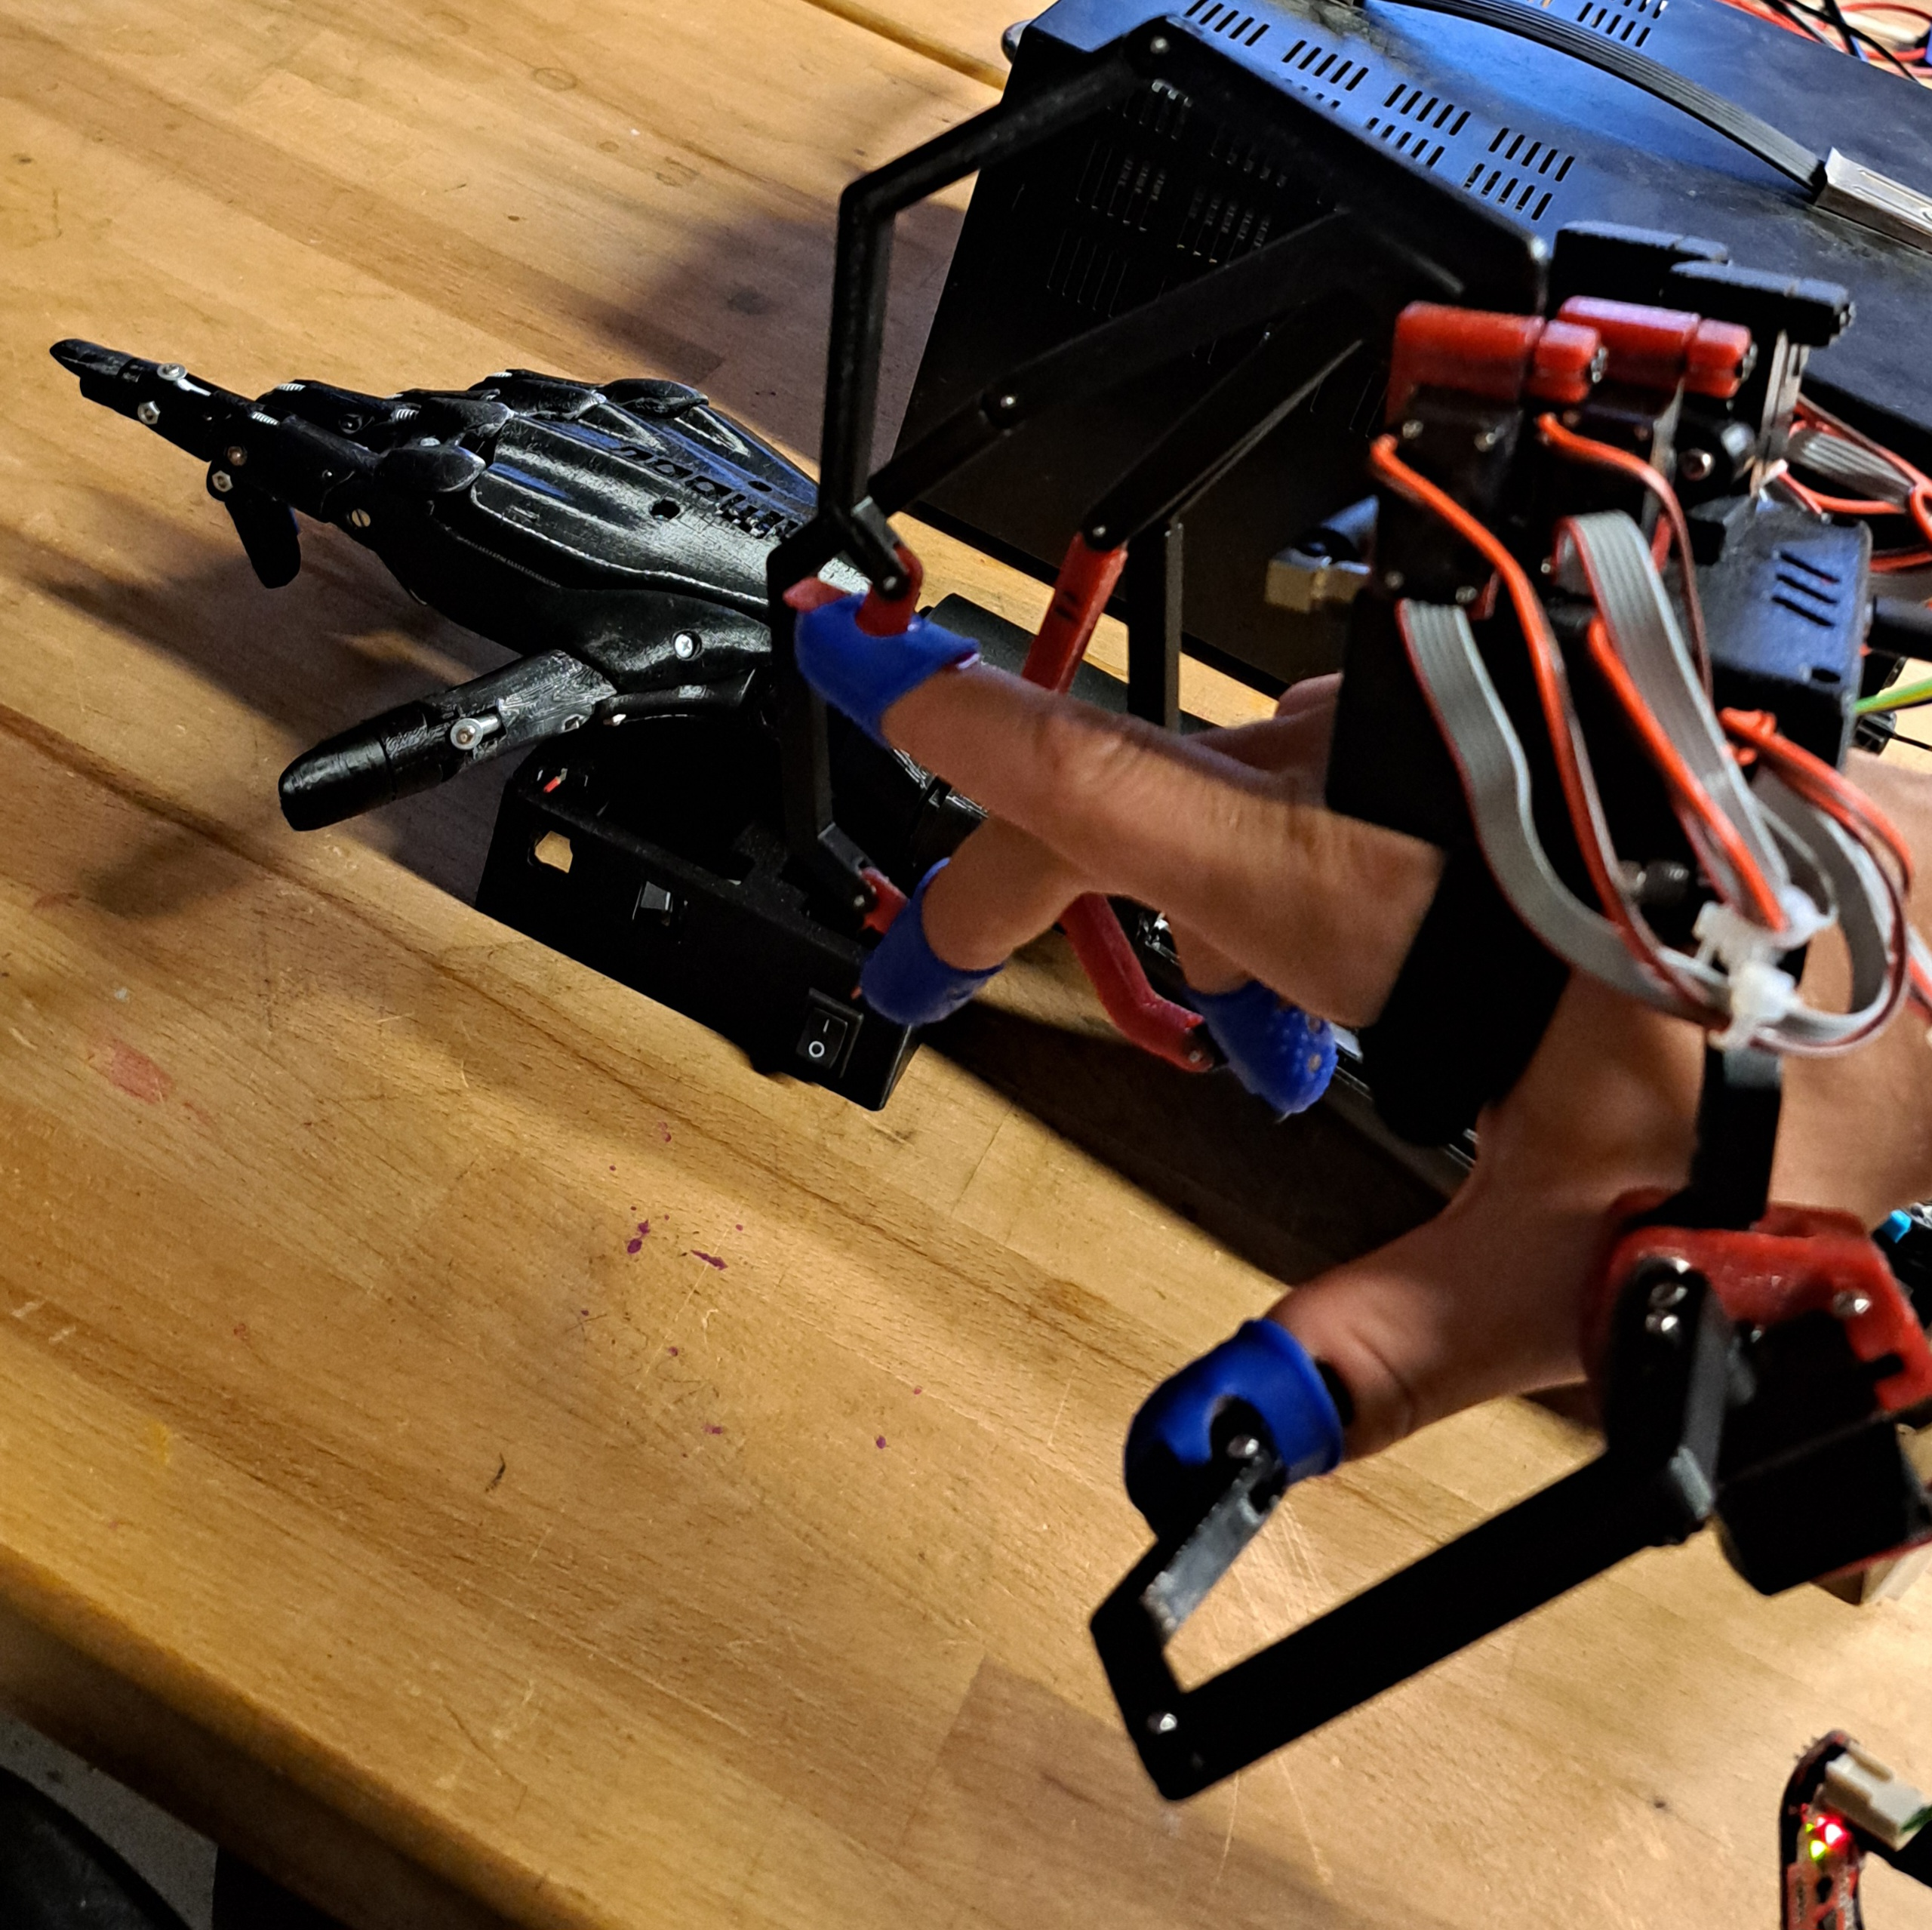
\includegraphics[width=0.82\textwidth]{Mirror_dukaz.jpg}
\caption{Praktické ověření režimu MIRROR při kopírování polohy prstů rukavice robotickou rukou.}
\label{fig:mirror-dukaz}
\end{figure}

Průměrná reakce při zavření byla 134{,}8~ms a průměrná reakce při otevření byla 126{,}4~ms. Plynulost pohybu a opakovatelnost byly hodnoceny jako velmi dobré. Bluetooth spojení bylo během testu stabilní. Subjektivní ovladatelnost byla hodnocena 5/5.

\subsection{Dynamická odezva v režimu EMG}
\label{subsec:dynamika-emg}

Výsledky měření M4 pro režim EMG jsou uvedeny v tabulce~\ref{tab:emg-otevrit-zavrit}. U všech pokusů bylo zaznamenáno, že udržování svalové aktivace při sevření bylo nekomfortní a po otevření trvalo přibližně 1,5~s, než serva zcela utichla.

\begin{table}[H]
\centering
\caption{Dynamická odezva v režimu EMG}
\label{tab:emg-otevrit-zavrit}
\begin{tabular}{|p{0.07\textwidth}|p{0.13\textwidth}|p{0.13\textwidth}|p{0.13\textwidth}|p{0.13\textwidth}|p{0.28\textwidth}|}
\hline
\textbf{Pokus} & \textbf{Reakce zavření [ms]} & \textbf{Ustálení zavření [ms]} & \textbf{Reakce otevření [ms]} & \textbf{Ustálení otevření [ms]} & \textbf{Poznámka} \\
\hline
1 & 670 & přibližně 1000 & 216 & přibližně 500 & Po otevření serva doznívala přibližně 1,5~s. \\
\hline
2 & 548 & přibližně 1000 & 418 & přibližně 500 & Pozorování odpovídalo pokusu 1. \\
\hline
3 & 500 & přibližně 1000 & 1200 & přibližně 500 & Pozorování odpovídalo pokusu 1. \\
\hline
4 & 548 & přibližně 1000 & 572 & přibližně 500 & Pozorování odpovídalo pokusu 1. \\
\hline
5 & 466 & přibližně 1000 & 360 & přibližně 500 & Pozorování odpovídalo pokusu 1. \\
\hline
\end{tabular}
\end{table}

Praktické provedení dynamického testu v režimu EMG je zachyceno na obr.~\ref{fig:emg-dukaz}. Fotografie ukazuje současné použití elektrod na předloktí, rukavice a robotické ruky při řízení podle sEMG signálu.

\begin{figure}[H]
\centering
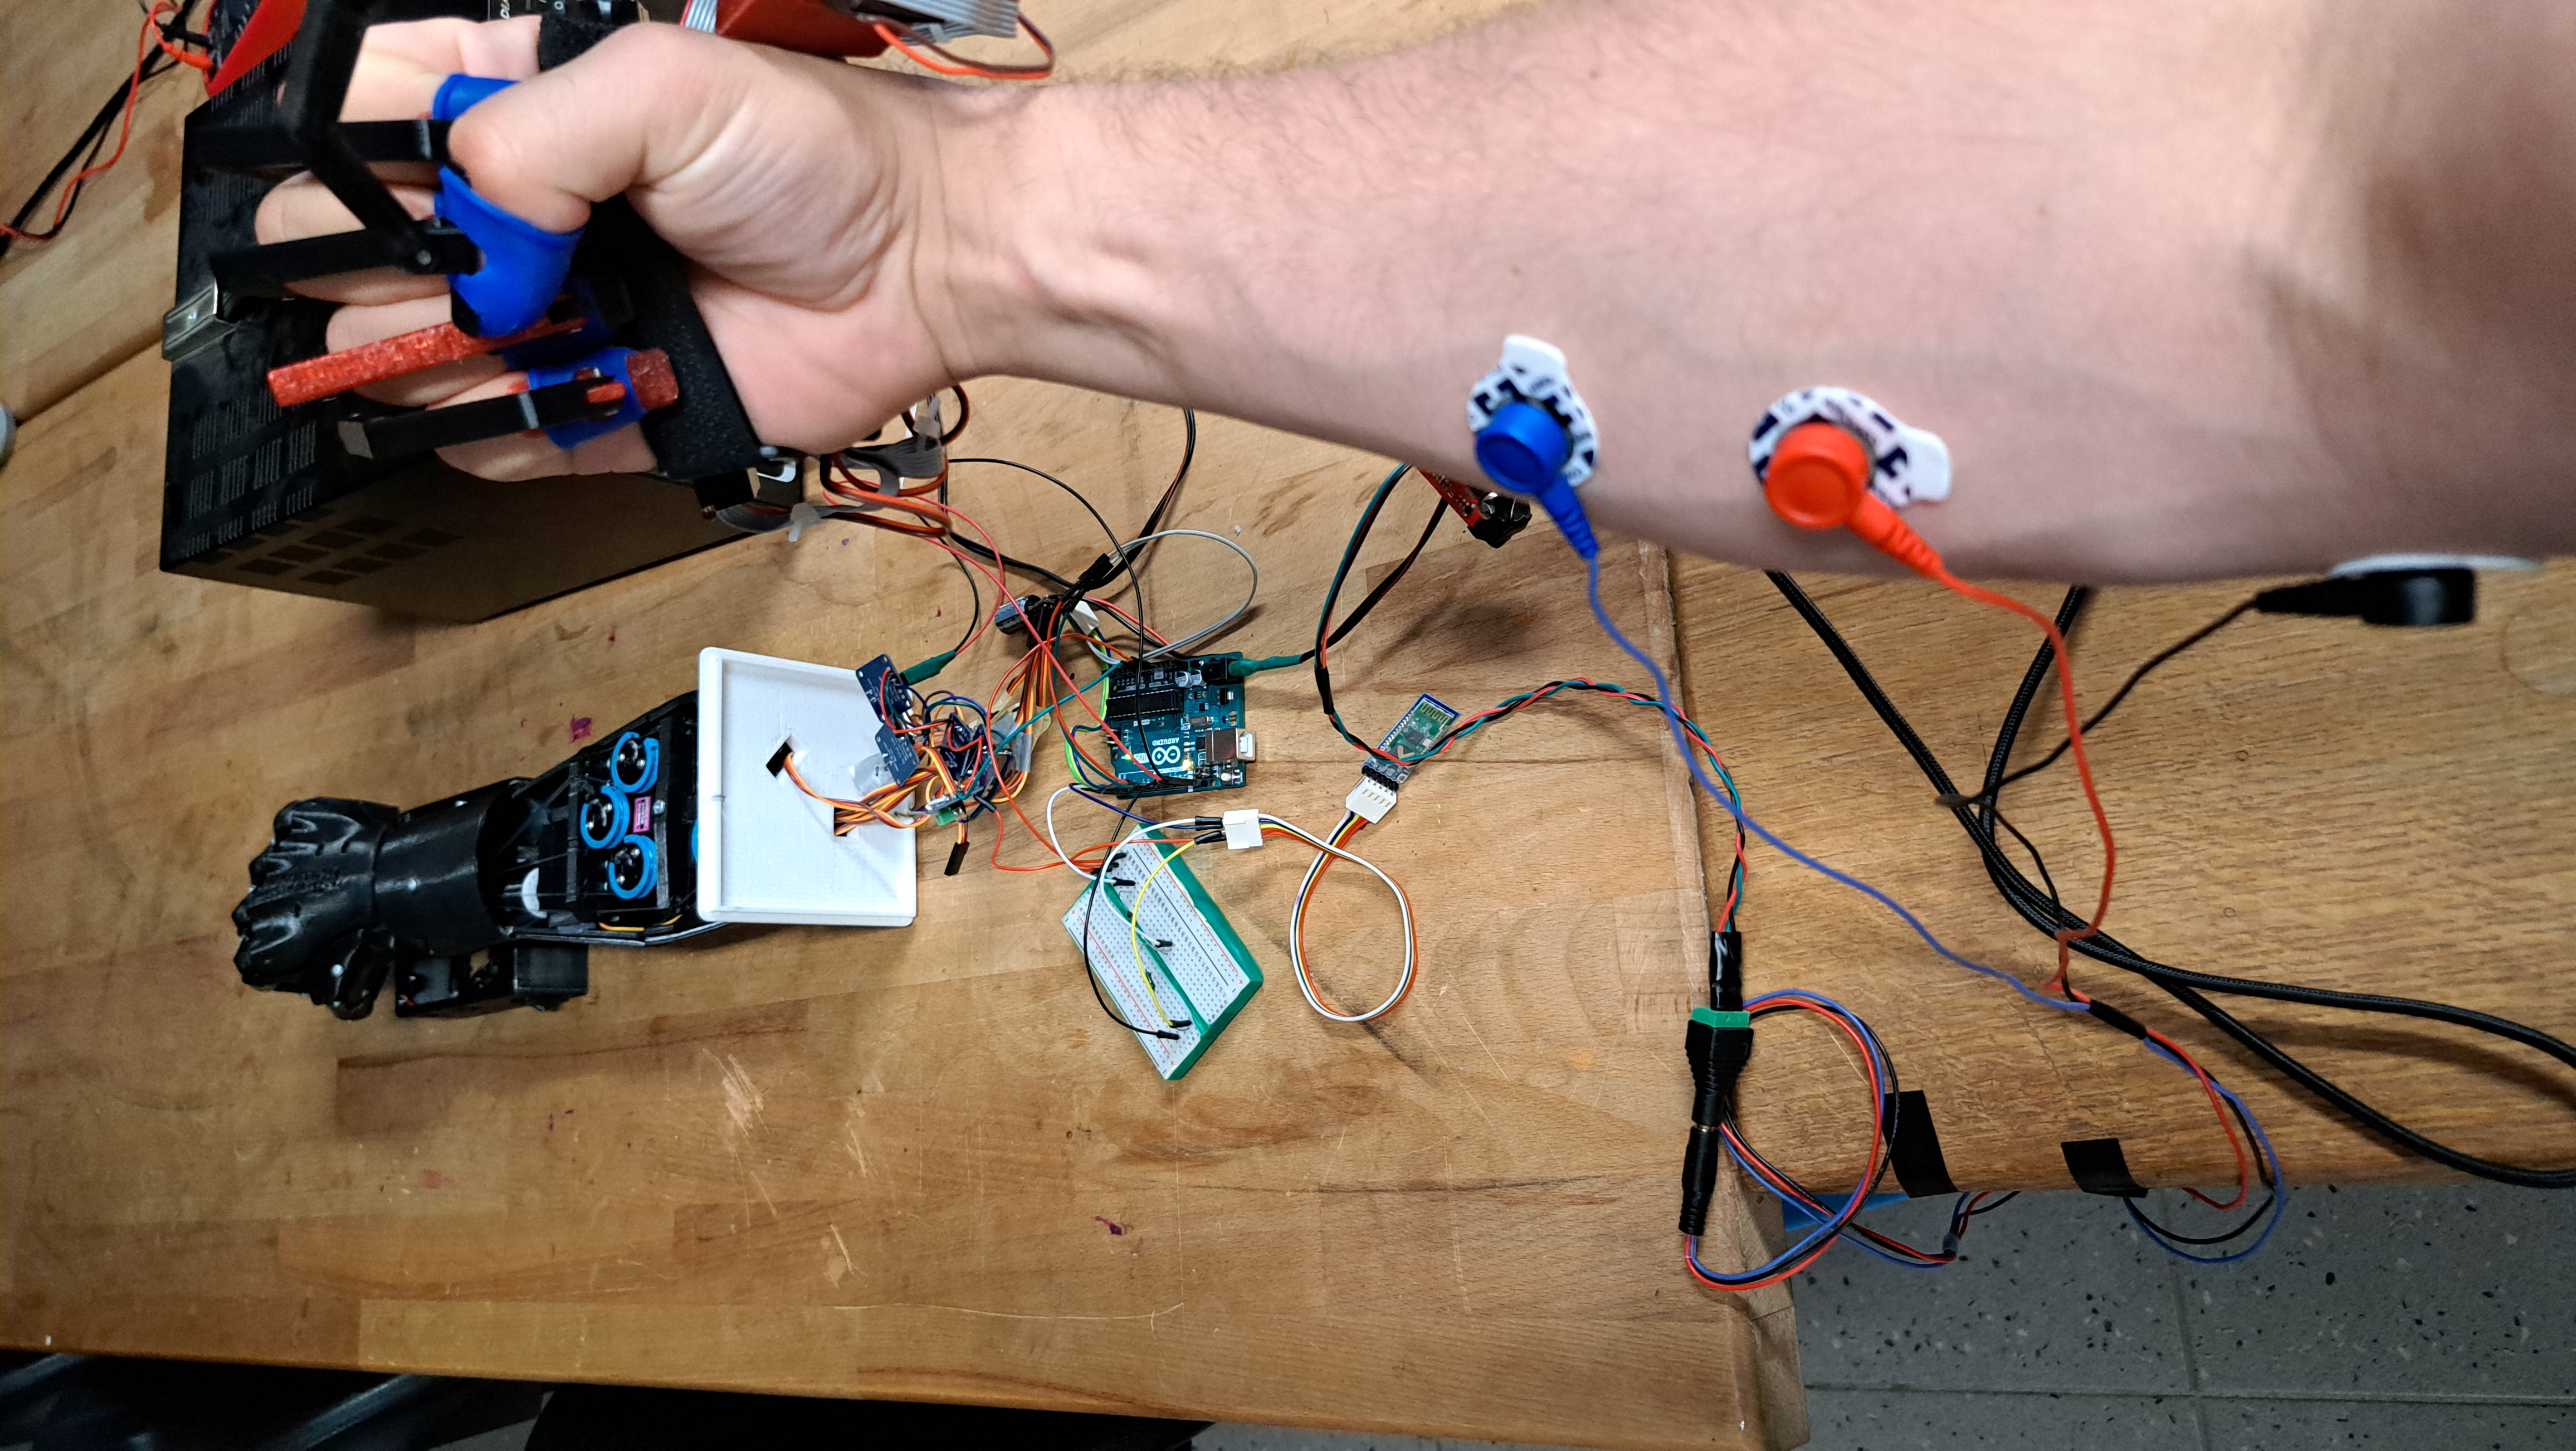
\includegraphics[width=0.82\textwidth]{EMG_dukaz.jpg}
\caption{Praktické ověření režimu EMG při řízení robotické ruky signálem z předloktí.}
\label{fig:emg-dukaz}
\end{figure}

Průměrná reakce při zavření byla 546{,}4~ms a průměrná reakce při otevření byla 553{,}2~ms. Typická doba ustálení při zavření byla přibližně 1000~ms, zatímco typická doba ustálení při otevření byla přibližně 500~ms. Plynulost i opakovatelnost byly hodnoceny jako špatné. Bluetooth spojení bylo během testu stabilní. Subjektivní ovladatelnost byla hodnocena 2/5.

\subsection{Porovnání dynamické odezvy}
\label{subsec:porovnani-dynamiky}

Režim MIRROR dosáhl v dynamickém testu výrazně kratších reakčních časů než režim EMG\@. Při zavírání byla průměrná reakce režimu MIRROR 134{,}8~ms, zatímco u režimu EMG 546{,}4~ms. Při otevírání byla průměrná reakce režimu MIRROR 126{,}4~ms, zatímco u režimu EMG 553{,}2~ms.

Režim EMG byl subjektivně rychlý pouze v okamžiku, kdy se podařilo vyvolat správnou svalovou aktivaci. V praxi byl však omezen nestabilitou sEMG signálu, pohybovými artefakty kabeláže a samovolnými aktivacemi. Režim MIRROR poskytoval plynulejší, přesnější a lépe opakovatelnou odezvu robotické ruky.

\section{Schopnost řízení mezilehlé polohy}
\label{sec:mezilehla-poloha}

Dalším testem byla schopnost dosáhnout přibližně 50~\% sevření robotické ruky a tuto polohu udržet po dobu 5~s. Testem bylo ověřeno jemné řízení, nikoli pouze přechod mezi krajními stavy otevřeno a zavřeno.

\subsection{Poloviční sevření v režimu MIRROR}
\label{subsec:polovicni-mirror}

\begin{table}[H]
\centering
\caption{Pokus o poloviční sevření v režimu MIRROR}
\label{tab:mirror-polovicni-sevreni}
\setlength{\tabcolsep}{2pt}
\begin{tabular}{|p{0.12\textwidth}|p{0.25\textwidth}|p{0.30\textwidth}|p{0.20\textwidth}|}
\hline
\textbf{Pokus} & \textbf{Dosažení 50~\%} & \textbf{Stabilita držení 5~s} & \textbf{Poznámka} \\
\hline
1 & snadné & stabilní & -- \\
\hline
2 & snadné & stabilní & -- \\
\hline
3 & snadné & mírné chvění & -- \\
\hline
4 & snadné & stabilní & -- \\
\hline
5 & snadné & stabilní & -- \\
\hline
\end{tabular}
\end{table}

Režimem MIRROR bylo možné snadno dosáhnout přibližně 50~\% sevření a tuto mezilehlou polohu udržet po dobu 5~s. Ve čtyřech z pěti pokusů bylo držení stabilní a v jednom pokusu bylo pozorováno pouze mírné chvění. Subjektivní jemná ovladatelnost byla hodnocena 5/5.

\subsection{Poloviční sevření v režimu EMG}
\label{subsec:polovicni-emg}

\begin{table}[H]
\centering
\caption{Pokus o poloviční sevření v režimu EMG}
\label{tab:emg-polovicni-sevreni}
\setlength{\tabcolsep}{2pt}
\begin{tabular}{|p{0.10\textwidth}|p{0.22\textwidth}|p{0.28\textwidth}|p{0.30\textwidth}|}
\hline
\textbf{Pokus} & \textbf{Dosažení 50~\%} & \textbf{Stabilita držení 5~s} & \textbf{Poznámka} \\
\hline
1 & obtížné & výrazné pohyby kolem 50~\% & -- \\
\hline
2 & nepodařilo se & žádná & Ruka přecházela z maxima do minima. \\
\hline
3 & nepodařilo se & žádná & Ruka přecházela z maxima do minima. \\
\hline
4 & obtížné & výrazné pohyby kolem 50~\% & -- \\
\hline
5 & nepodařilo se & žádná & Ruka zůstala ve staženém stisku. \\
\hline
\end{tabular}
\end{table}

V režimu EMG se nepodařilo spolehlivě dosáhnout ani udržet přibližně 50~\% sevření. Ve dvou pokusech bylo dosažení mezilehlé polohy obtížné a poloha výrazně kolísala. Ve třech pokusech se polohy dosáhnout nepodařilo. Subjektivní jemná ovladatelnost byla hodnocena 1/5.

\section{Praktické uchopení předmětů}
\label{sec:uchopeni-predmetu}

Praktická použitelnost obou režimů byla ověřována uchopováním tří předmětů: houbičky na nádobí, plastového meče a fixy. Hodnocena byla úspěšnost uchopení, čas do uchopení, vypadnutí předmětu, přílišné zmáčknutí a případné problémy s puštěním předmětu.

\subsection{Uchopení předmětu v režimu MIRROR}
\label{subsec:uchopeni-mirror}

\begin{table}[H]
\centering
\caption{Uchopení předmětu v režimu MIRROR}
\label{tab:mirror-uchopeni}
\setlength{\tabcolsep}{2pt}
\begin{tabular}{|p{0.17\textwidth}|p{0.11\textwidth}|p{0.11\textwidth}|p{0.13\textwidth}|p{0.13\textwidth}|p{0.25\textwidth}|}
\hline
\textbf{Předmět} & \textbf{Pokusy / úspěchy} & \textbf{Čas do uchopení} & \textbf{Vypadnutí předmětu} & \textbf{Přílišné zmáčknutí} & \textbf{Poznámka} \\
\hline
Houbička na nádobí & 3 / 3 & 500~ms & ne & ne & -- \\
\hline
Plastový meč & 3 / 2 & 500~ms & ano, jednou & ne & Omezením byl malý počet stupňů volnosti pro přizpůsobení tvaru předmětu. \\
\hline
Fixa & 3 / 2 & 1~s & ano & ne & Byl proveden pokus o úchop mezi prsty, nikoli sevření do dlaně. \\
\hline
\end{tabular}
\end{table}

V režimu MIRROR bylo praktické uchopení předmětů celkově úspěšné. Nejlepší výsledek byl dosažen u houbičky na nádobí, kde byly úspěšné všechny tři pokusy. U plastového meče a fixy byla úspěšnost 2/3. Subjektivní praktičnost režimu MIRROR byla hodnocena 4/5.

Neúspěchy souvisely spíše s mechanickými omezeními robotické ruky, zejména s menším počtem stupňů volnosti a omezenou schopností jemného úchopu mezi prsty, než s nestabilitou řízení.

\subsection{Uchopení předmětu v režimu EMG}
\label{subsec:uchopeni-emg}

\begin{table}[H]
\centering
\caption{Uchopení předmětu v režimu EMG}
\label{tab:emg-uchopeni}
\setlength{\tabcolsep}{2pt}
\begin{tabular}{|p{0.13\textwidth}|p{0.09\textwidth}|p{0.09\textwidth}|p{0.12\textwidth}|p{0.11\textwidth}|p{0.11\textwidth}|p{0.23\textwidth}|}
\hline
\textbf{Předmět} & \textbf{Pokusy / úspěchy} & \textbf{Čas do uchopení} & \textbf{Vypadnutí} & \textbf{Přílišné zmáčknutí} & \textbf{Problém s puštěním} & \textbf{Poznámka} \\
\hline
Houbička na nádobí & 3 / 1 & 1~s & ano & ano & ne & Úchop byl nestabilní při snaze o lehké sevření. \\
\hline
Plastový meč & 3 / 2 & 1~s & ano & nelze určit & ne & Předmět vypadl kvůli nechtěnému pohybu prstů. \\
\hline
Fixa & 3 / 0 & nelze určit & ano & nelze určit & ne & Úchop se nepodařil. \\
\hline
\end{tabular}
\end{table}

\begin{figure}[H]
\centering
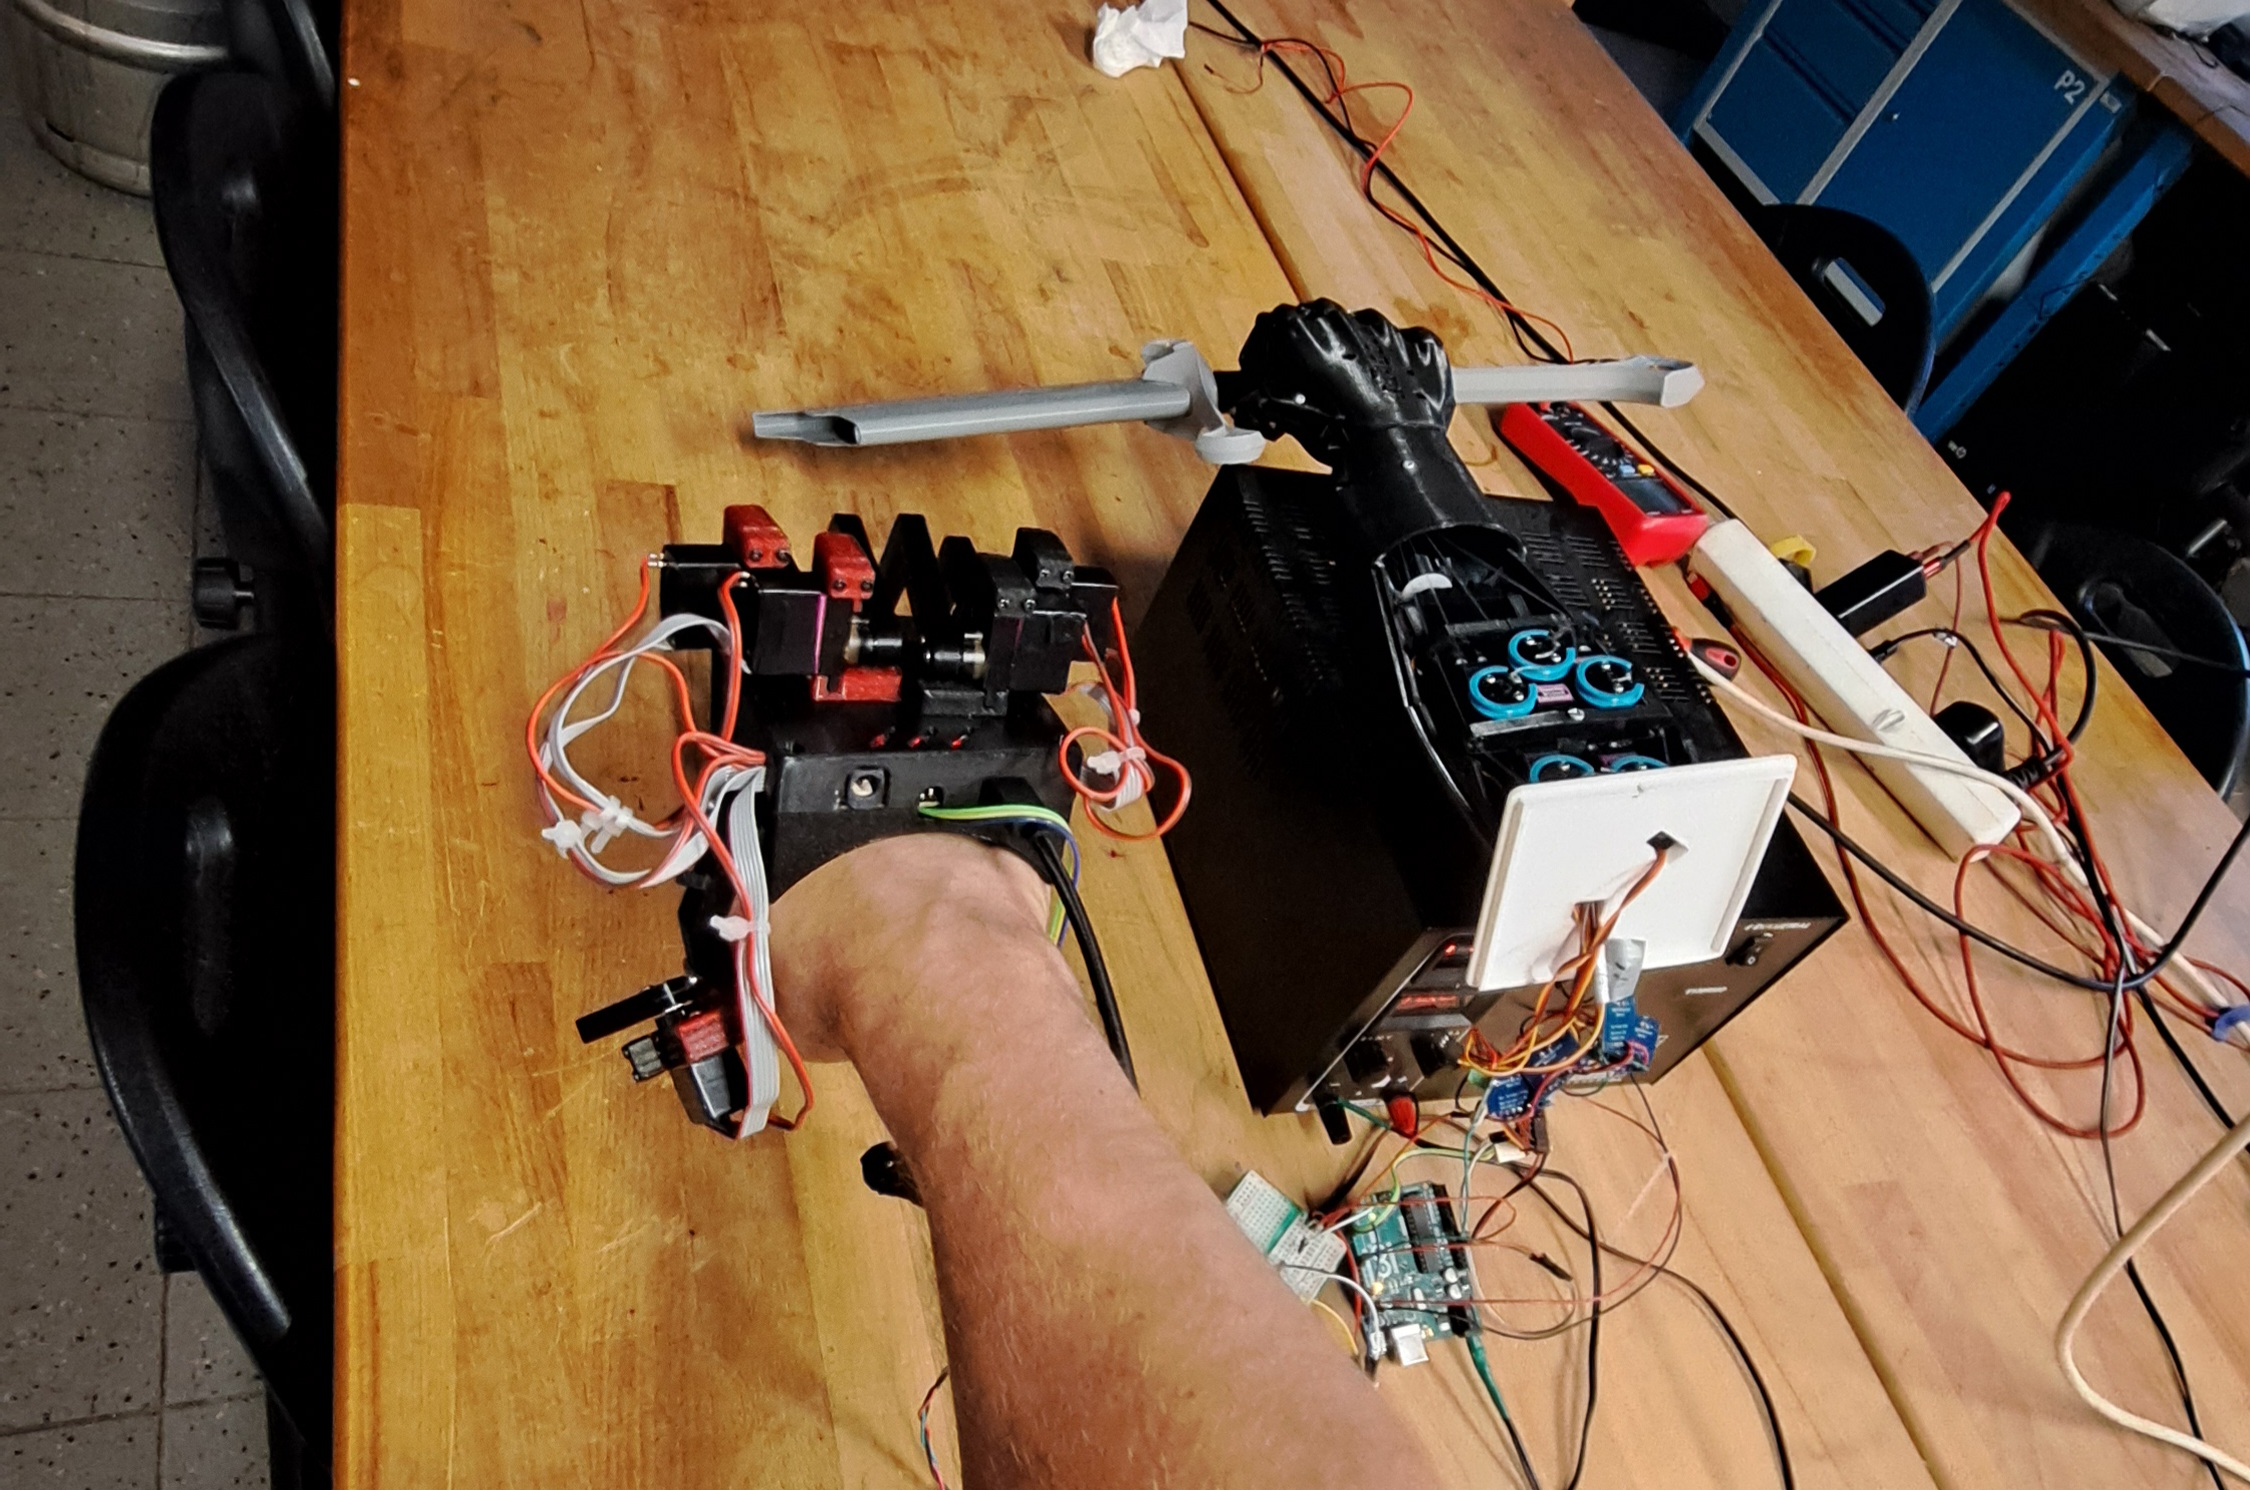
\includegraphics[width=0.9\textwidth]{drzi_mec.jpg}
\caption{Testování držení plastového meče.}
\end{figure}

V režimu EMG bylo praktické uchopení předmětů výrazně méně spolehlivé než v režimu MIRROR\@. Houbičku na nádobí se podařilo úspěšně uchopit pouze v jednom ze tří pokusů, plastový meč ve dvou ze tří pokusů a fixu se nepodařilo uchopit vůbec. Subjektivní praktičnost režimu EMG byla hodnocena 2/5.

Režim EMG byl při uchopování použitelný pouze omezeně, zejména kvůli nestabilnímu úchopu, nechtěným pohybům a obtížnému udržení jiné než krajní polohy.

\subsection{Porovnání úspěšnosti uchopení}
\label{subsec:uchopeni-porovnani}

Celková úspěšnost uchopení byla v režimu MIRROR 7/9 (78~\%), zatímco v režimu EMG pouze 3/9 (33~\%). Oba režimy dosáhly srovnatelného času do uchopení (500~ms vs. 1~s), avšak EMG vykazoval výrazně vyšší výskyt vypadnutí předmětu a nestabilního úchopu. Neúspěchy v režimu MIRROR byly přičítány mechanickým omezením robotické ruky, zatímco v režimu EMG šlo primárně o nestabilitu řídicího signálu. Subjektivní praktičnost byla hodnocena 4/5 pro MIRROR a 2/5 pro EMG\@.

\section{Analýza rušení EMG signálu}
\label{sec:ruseni-emg}

Měření M9 bylo zaměřeno na pozorování rušení EMG signálu. V klidu bez pohybu kabelů docházelo k občasné aktivaci. Pohyb kabelů sEMG měl výrazný vliv na chování systému. Přiblížení k napájení nebo elektronice mělo menší vliv. Nejčastějším projevem rušení bylo cukání a samovolné zavření robotické ruky. Bluetooth spojení bylo během testu stabilní.

Bylo zaznamenáno, že senzor MyoWare neměl kabely připojené napevno. Při pohybu se proto kabely mohly pohybovat a způsobovat rušení nebo úplné přerušení signálu. Subjektivní odolnost EMG proti rušení byla hodnocena 1/5.

Pozorované problémy byly přisouzeny primárně sEMG signálu a kabeláži, nikoli komunikaci mezi deskami. Tato interpretace byla podpořena tím, že Bluetooth spojení zůstalo během měření stabilní.

\section{Subjektivní hodnocení režimů řízení}
\label{sec:subjektivni-hodnoceni}

Po dokončení dílčích měření bylo provedeno subjektivní hodnocení obou režimů. Hodnocena byla přirozenost ovládání, přesnost, rychlost, únava, pocit kontroly, praktičnost pro uchopení předmětů a celkové hodnocení. U kritéria únavy znamenala hodnota 1 velkou únavu a hodnota 5 stav bez únavy.

\begin{table}[H]
\centering
\caption{Subjektivní hodnocení režimů MIRROR a EMG}
\label{tab:subjektivni-hodnoceni}
\begin{tabular}{|p{0.55\textwidth}|p{0.17\textwidth}|p{0.17\textwidth}|}
\hline
\textbf{Kritérium} & \textbf{MIRROR} & \textbf{EMG} \\
\hline
Přirozenost ovládání & 4/5 & 2/5 \\
\hline
Přesnost & 5/5 & 1/5 \\
\hline
Rychlost & 4/5 & 4/5 \\
\hline
Únava & 3/5 & 2/5 \\
\hline
Pocit kontroly & 3/5 & 2/5 \\
\hline
Praktičnost pro uchopení předmětů & 5/5 & 2/5 \\
\hline
Celkové hodnocení & 4/5 & 2/5 \\
\hline
\end{tabular}
\end{table}

Režim MIRROR byl slovně hodnocen jako dobrý základ pro teleoperativní úlohy. Režim EMG byl hodnocen jako funkční, ale pro spolehlivé řízení vyžadující další odladění více částí systému. Subjektivní hodnocení potvrdilo objektivní pozorování z dílčích testů: MIRROR byl hodnocen lépe v přesnosti, přirozenosti i praktičnosti uchopení.

\section{Diskuse výsledků}
\label{sec:diskuse-vysledku}

Testováním bylo ukázáno, že režim MIRROR poskytoval výrazně spolehlivější, přesnější a lépe opakovatelné řízení robotické ruky než režim EMG\@. V dynamickém testu otevřít--zavřít--otevřít měl MIRROR průměrnou reakci přibližně 135~ms při zavření a 126~ms při otevření. Pohyb byl plynulý, dobře opakovatelný a Bluetooth spojení bylo stabilní.

Dosažené reakční doby v režimu MIRROR jsou z hlediska plynulosti teleoperace příznivé. Literatura uvádí, že výrazný pokles výkonnosti systému nastupuje při latencích nad 400~ms a přechod operátora na diskontinuální strategii řízení je typický při zpožděních nad 1~s \cite{Bolarinwa2022,Almeida202098}. Naměřené hodnoty 135~ms a 126~ms jsou tedy výrazně pod kritickou hranicí, ačkoli jsou vyšší než limity doporučované pro nejnáročnější haptické aplikace (1--5~ms) nebo chirurgické teleoperace (pod 105~ms) \cite{Aijaz2018,Almeida202098}. Pro scénář demonstrační teleoperace robotické ruky jsou však dosažené latence adekvátní \cite{Brazdil2020,Almeida202098}.

Režim EMG měl ve stejném testu průměrnou reakci přibližně 546~ms při zavření a 553~ms při otevření. Prakticky byl však výrazně omezen nestabilitou sEMG signálu, pohybovými artefakty kabeláže a samovolnými aktivacemi. Jemné řízení mezilehlé polohy bylo u EMG nespolehlivé.

Horší výsledky EMG režimu jsou v souladu s literaturou. Jednokanálový přístup je hodnocen jako vhodný pouze pro binární nebo proporcionální řízení jedné funkce, přičemž přesnost klasifikace pro jednotlivé prsty dosahuje v nízkonákladových systémech pouze kolem 50\,\%, zatímco pro celou ruku (sevření dlaně) 80--90\,\% \cite{Brazdil2020,Safran2022}. Omezení na jeden kanál bylo v realizovaném systému záměrné: cílem bylo ověřit, zda je binární detekce sevření zvládnutelná v podmínkách prototypového zapojení s nestíněnou kabeláží a jednoduchou kalibrací. Alternativní vícekanálový přístup by přinesl vyšší přesnost, ale zároveň vyšší hardwarovou a kalibrační náročnost \cite{Brazdil2020,Sul2025627,Wu2024613}.

EMG řízení má oproti polohovému přístupu principiální výhodu: sEMG signál se objevuje přibližně 50--100~ms před skutečným fyzickým pohybem, což umožňuje systému předvídat záměr uživatele \cite{Song2023823,Xiong2024}. Tato výhoda se v realizovaném systému neprosadila, protože ji překryly nedostatky v kvalitě zapojení, nikoli samotná nevýhodnost sEMG jako řídicího principu. Pro osoby po amputaci nebo s motorickými omezeními je EMG řízení navíc jedinou prakticky dostupnou metodou ovládání robotické protézy \cite{Brazdil2020,Najman2017}.

Při uchopování předmětů byl režim MIRROR použitelnější a praktičtější. Umožnil přirozenější dávkování sevření a lepší kontrolu nad okamžikem uchopení i puštění předmětu. Režim EMG byl použitelný pouze omezeně, zejména kvůli nestabilnímu úchopu a obtížnému udržení jiné než krajní polohy.

Bluetooth spojení bylo během měření stabilní. Pozorované problémy EMG řízení proto nebyly přisuzovány komunikaci mezi deskami, ale především kvalitě sEMG vstupu, mechanickému namáhání kabelů a citlivosti senzoru MyoWare 1.0 na pohybové artefakty.

Souběžná činnost režimů MIRROR a EMG byla vyhodnocena jako potenciálně přínosná. Z hlediska řešené problematiky může sEMG poskytovat doplňující informaci využitelnou ke zlepšení silové zpětné vazby, odhadu únavy uživatele nebo řízení aktivní asistence rukavice. Literatura v tomto smyslu doporučuje hybridní přístupy kombinující EMG s dalšími senzory (IMU, tlakové senzory) pro dosažení spolehlivějšího řízení \cite{Sul2025627,Xiong2024}. Pro samotné řízení robotické ruky však testováním nebyl prokázán jasný důvod, proč by v aktuální podobě mělo sEMG nahrazovat řízení pomocí rukavice. Souběžná činnost MIRROR a EMG proto byla vyhodnocena jako perspektivní spíše pro doplňkovou analýzu než jako přímá náhrada polohového řízení.

\section{Dílčí závěr experimentální kapitoly}
\label{sec:dilci-zaver-experimenty}

Experimentálním testováním bylo prokázáno, že v aktuální podobě systému je režim MIRROR vhodnější pro řízení robotické ruky než režim EMG\@. Režim MIRROR vykazoval kratší reakční dobu, lepší opakovatelnost, vyšší stabilitu v klidu, lepší jemnou ovladatelnost a vyšší praktickou úspěšnost při uchopování předmětů.

Režim EMG byl funkční, avšak jeho praktické použití bylo výrazně omezeno nestabilitou sEMG signálu, pohybovými artefakty kabeláže a samovolnými aktivacemi. Souběžné využití EMG a MIRROR může být perspektivní zejména jako doplněk pro vyhodnocení únavy, podporu aktivní asistence rukavice nebo budoucí rozšíření silové zpětné vazby. V aktuální podobě však nebylo vhodné chápat EMG jako přímou náhradu řízení podle polohy prstů v rukavici.
%7
\chapter{Závěr}
Cílem této diplomové práce bylo navrhnout, sestavit a~experimentálně ověřit bilaterální teleoperační systém pro řízení robotické ruky doplněný o~haptickou silovou zpětnou vazbu. Všechny stanovené cíle byly splněny. Byla zprovozněna haptická rukavice Remote Feelings, na jejím základě byl vytvořen silový zpětnovazební řetězec mezi robotickou rukou a~operátorem, bylo realizováno a~vzájemně porovnáno řízení pomocí polohového snímání a~pomocí sEMG a~celý systém byl propojen bezdrátově. Výsledkem je funkční, bezdrátově propojená
sestava složená ze senzoriky sEMG, robotické ruky InMoov, hardwaru pro
haptickou odezvu, dvou řídicích desek a~příslušného firmwaru, čímž byl naplněn i~požadovaný výstup práce.

Experimentální testování porovnalo dva režimy řízení robotické ruky. Polohové zrcadlení (MIRROR) se ukázalo jako velmi spolehlivé: dosahovalo průměrné reakční doby přibližně 135~ms při zavírání a~126~ms při otevírání, vykazovalo vysokou stabilitu v~klidu, dobrou opakovatelnost a~umožňovalo i~jemné řízení mezilehlých poloh; při praktickém uchopování předmětů dosáhl tento režim úspěšnosti 78~\%. Myoelektrický režim (EMG) byl funkční a~v~okamžiku správné svalové aktivace rychlý, jeho praktická spolehlivost však byla nižší, což
odpovídá vlastnostem jednokanálového sEMG řízení popsaným v~odborné literatuře. Toto chování nebylo dáno nevhodností sEMG jako principu, nýbrž záměrným omezením na jediný analogový kanál a~podmínkami prototypového zapojení s~nestíněnou kabeláží; vícekanálové řešení by přesnost zvýšilo za cenu vyšší hardwarové a~kalibrační náročnosti. Naměřené reakční doby polohového režimu se přitom pohybují výrazně pod hranicí, od níž literatura uvádí pokles výkonnosti teleoperace, a~jsou tedy pro demonstrační scénář plně dostačující.

Na základě dosažených výsledků lze odpovědět na výzkumné otázky práce.

První otázka se týkala vzájemných výhod obou způsobů řízení a~přínosu jejich souběžné činnosti. Polohové řízení rukavicí poskytuje vyšší přesnost, stabilitu, opakovatelnost a~přirozenější dávkování úchopu, a~je proto vhodnější pro samotné teleoperační vedení pohybu robotické ruky. Myoelektrické řízení má naopak principiální výhodu v~tom, že se signál objevuje přibližně 50 až~100~ms před vlastním pohybem svalu, což umožňuje predikci pohybového záměru; zároveň zůstává jedinou prakticky dostupnou modalitou pro osoby po amputaci nebo s~motorickým
omezením. Souběžná činnost obou přístupů se ukázala jako perspektivní především jako doplněk~--- sEMG může poskytovat informaci pro odhad svalové únavy, řízení aktivní asistence rukavice nebo zpřesnění silové zpětné vazby~--- spíše než jako přímá náhrada polohového řízení.

Druhá otázka směřovala k~volbě zpětnovazební veličiny a~místu jejího měření. Jako vstup pro zpětnou vazbu byl zvolen proudový odběr servomotorů robotické ruky, měřený senzory INA219 na straně vykonávacího systému (Follower). Z~filtrovaného nadproudu vůči adaptivní základní hladině byl odvozen kontakt a~jeho intenzita, které byly přeneseny zpět do rukavice a~převedeny na haptický odpor proti pohybu prstu. Toto nepřímé snímání nevyžaduje senzory přímo   ~místě
kontaktu a~je konstrukčně robustní; jeho citlivost při prvotním doteku byla v~souladu s~doporučením literatury posílena fúzí s~FSR senzory, filtrací a~hysterezí, čímž byla detekce kontaktu spolehlivě zajištěna.

Třetí otázka se zabývala výhodami a~nevýhodami bezdrátového propojení komponent. Bezdrátové spojení Bluetooth~Classic prostřednictvím modulu HC-05 přineslo jednoduchost integrace, emulaci sériové linky bez nutnosti aplikačního protokolu a~odstranění kabeláže mezi oběma subsystémy. Jeho nevýhodou je oproti alternativám (ESP-NOW, Wi-Fi) vyšší přenosová latence a~nižší propustnost, navíc omezená rychlostí UART 9600~Bd, která ale byla nezbytná pro správný chod softwaru. Na demonstrační vzdálenost do jednoho metru se však tyto nevýhody neprojevily jako limitující a~spojení bylo během veškerého testování stabilní. Pro aplikace s přísnějšími nároky na latenci je přirozeným rozšířením přechod na ESP-NOW, což by u stávajícího projektu znamenalo nahradit v robotické ruce Arduino UNO vývojovou deskou s mikrokontrolérem s Wi-Fi od Espressif.

Silnou stránkou práce je komplexní integrace celého řetězce~--- od mechaniky přes elektroniku a~firmware až po experimentální ověření~--- do jediného funkčního teleoperačního systému postaveného převážně z~nízkonákladových a~open-source komponent. Realizace propojila řadu inženýrských úloh, které jsem v takovém spektru a rozsahu řešil poprvé: 3D~tisk mechanických dílů, fyzické pájení plošných spojů, práci s elektronikou, se kterou jsem nikdy předtím nepracoval (ESP32, INA219, FSR, H-můstky uvnitř servomotorů) a~programování vestavných systémů v~novém vývojovém prostředí a~jazyce. Zvládnutí a~vzájemné propojení těchto oblastí do spolehlivě fungujícího celku představovalo hlavní osobní inženýrskou výzvu a~zároveň její významný přínos z~hlediska osvojených dovedností a získaných zkušeností.

Mezi oblasti s~prostorem pro další rozvoj patří
\begin{itemize}
    \item vylepšení mechanických částí, aby se snížilo tření, snížila deformace a~zvýšil rozsah pohybu,
    \item doplnění kontrolního součtu (CRC) do komunikačního protokolu,
    \item zvýšení přenosové rychlosti a~přechod na nízkolatenční bezdrátový protokol,
    \item stínění a~pevné vedení sEMG kabeláže pro potlačení pohybových artefaktů (nebo přechod i zde na bezdrátové řešení),
    \item a~rozšíření myoelektrického řízení na více kanálů.
\end{itemize}     
Tyto kroky by umožnily plněji využít prediktivní potenciál sEMG a~dále zvýšit věrnost silové zpětné vazby. Práce nicméně prokázala, že i~z~dostupných open-source~nízkonákladových prostředků lze sestavit funkční bilaterální teleoperační systém se silovou zpětnou vazbou, a~vytvořila spolehlivý hardwarový i~softwarový základ pro jeho další rozvoj.




\printbibliography[title={Použitá literatura},heading=bibintoc] % sazba seznamu citací a vložení do obsahu 
% \printbibliography[title={References},heading=bibintoc] 

% \addcontentsline{toc}{chapter}{References} 
%%%%%%%%%%%%%%%%%%%%%%%%%%%%%%%%%%%%%%%%%%%%%%%%%%%%%%%%%%%%%%%%%%%%%%%%%%%%%%%%%%


\renewcommand{\indexname}{Přehled příkazů, prostředí a voleb}
\printindex

\appendix % začátek příloh / beginning of appendiecies
\chapter{Přílohy}
\section{Obsah vloženého balíku do IS/STAG TUL} % příklad přílohy 
\begin{itemize}
    \item Text práce 
    \item Dva PlatformIO projekty. Jeden pro ESP32 rukavici s sEMG (Remote\_Feelings\_sEMG) a druhý pro Arduino UNO robotickou ruku s blueetooth modulem (InMoov\_BT)
    \item Podrobný návod jak ve VS Code s PlatformIO otevřít, nahrát a spustit oba projekty
\end{itemize}

\end{document}
